%!TEX program = xelatex

% Name           : defense.tex
% Author         : Jarrett Keifer (jkeifer0@gmail.com)
% Version        : 0.4
% Created on     : 05.05.2013
% Last Edited on : 24.03.2014
% Copyright      : Copyright (c) 2013-2014 by Benjamin Weiss. All rights reserved.
% License        : This file may be distributed and/or modified under the
%                  GNU Public License.
% Description    : HSRM beamer theme demonstration. Also includes a short 
%                  Tutorial regarding the beamer class.

\documentclass[draft,compress]{beamer}

% if handout option for beamer, make 4-up landscape
\mode<handout>{%
  \usepackage{pgfpages}%
  \pgfpagesuselayout{4 on 1}[letterpaper,border shrink=5mm, landscape]}

%--------------------------------------------------------------------------
% Common packages
%--------------------------------------------------------------------------
\usepackage[australian, american]{babel}
\usepackage{datetime}
\setdefaultdate{\dateaustralian}

\newdateformat{noyear}{\THEDAY\ \monthname[\THEMONTH]}
\newdateformat{aagdate}{\THEDAY\ \monthname[\THEMONTH]\ \THEYEAR}

% command to print noyear dates, args {dayno}{monthno}
\newcommand{\datenoyear}[2]{%
  \noyear\formatdate{#1}{#2}{1}%
  \aagdate}
  

\usepackage[overload]{textcase} %provides capitalization protection via \NoCaseChange tag

%\usepackage{tikz}
%\usepackage{tikzscale}
\usepackage{pgf}  % for plots
\usepackage{setspace}

\usepackage[export]{adjustbox}  % for right align of figures

% Reference Settings
% *************** Set Biblatex Style and Options ***************

\usepackage{csquotes}
\usepackage[authordate-trad, backend=biber, firstinits=true, maxcitenames=3, isbn=false, doi=false, eprint=false, shorthandfull, sorting=nyt, sortcites=true, ibidtracker=false, abbreviate=true]{biblatex-chicago}
\addbibresource[datatype=bibtex]{thesis.bib}

%Check for page range in postnotes to use a colon not comma
\renewcommand{\postnotedelim}{\iffieldpages{postnote}{\addcolon\space}{\addcomma\space}} 
\DeclareFieldFormat{postnote}{#1} 

%Fix date format in bib -- could be moved to external .lbx file (with comments; change DefineBib... to DeclareBib...)
%%%%\DeclareLanguageMapping{american}{american-dmy}
%%%%
%%%%\begin{filecontents}{american-dmy.lbx}
%%%%\ProvidesFile{american-dmy.lbx}[american localisation with dmydate format for long dates]
%%%%
%%%%\InheritBibliographyExtras{american}
\DefineBibliographyExtras{american}{%
  \protected\def\mkbibdatelong#1#2#3{%
    \iffieldundef{#3}
      {}
      {\stripzeros{\thefield{#3}}%
       \iffieldundef{#2}{}{\nobreakspace}}%
    \iffieldundef{#2}
      {}
      {\mkbibmonth{\thefield{#2}}%
       \iffieldundef{#1}{}{\space}}%
    \iffieldbibstring{#1}{\bibstring{\thefield{#1}}}{\stripzeros{\thefield{#1}}}}%
}
%%%%\InheritBibliographyStrings{american}
%%%%\endinput
%%%%\end{filecontents}

% *************** Make ref links whole ref in text *****************
%%%%\DeclareCiteCommand{\cite}
%%%%  {\usebibmacro{prenote}}
%%%%  {\usebibmacro{citeindex}%
%%%%   \printtext[bibhyperref]{\usebibmacro{cite}}}
%%%%  {\multicitedelim}
%%%%  {\usebibmacro{postnote}}
%%%%
%%%%\DeclareCiteCommand*{\cite}
%%%%  {\usebibmacro{prenote}}
%%%%  {\usebibmacro{citeindex}%
%%%%   \printtext[bibhyperref]{\usebibmacro{citeyear}}}
%%%%  {\multicitedelim}
%%%%  {\usebibmacro{postnote}}
%%%%
%%%%\DeclareCiteCommand{\parencite}[\mkbibparens]
%%%%  {\usebibmacro{prenote}}
%%%%  {\usebibmacro{citeindex}%
%%%%    \printtext[bibhyperref]{\usebibmacro{cite}}}
%%%%  {\multicitedelim}
%%%%  {\usebibmacro{postnote}}
%%%%
%%%%\DeclareCiteCommand*{\parencite}[\mkbibparens]
%%%%  {\usebibmacro{prenote}}
%%%%  {\usebibmacro{citeindex}%
%%%%    \printtext[bibhyperref]{\usebibmacro{citeyear}}}
%%%%  {\multicitedelim}
%%%%  {\usebibmacro{postnote}}
%%%%
%%%%\DeclareCiteCommand{\footcite}[\mkbibfootnote]
%%%%  {\usebibmacro{prenote}}
%%%%  {\usebibmacro{citeindex}%
%%%%  \printtext[bibhyperref]{ \usebibmacro{cite}}}
%%%%  {\multicitedelim}
%%%%  {\usebibmacro{postnote}}
%%%%
%%%%\DeclareCiteCommand{\footcitetext}[\mkbibfootnotetext]
%%%%  {\usebibmacro{prenote}}
%%%%  {\usebibmacro{citeindex}%
%%%%   \printtext[bibhyperref]{\usebibmacro{cite}}}
%%%%  {\multicitedelim}
%%%%  {\usebibmacro{postnote}}
%%%%
%%%%\DeclareCiteCommand{\textcite}
%%%%  {\boolfalse{cbx:parens}}
%%%%  {\usebibmacro{citeindex}%
%%%%   \printtext[bibhyperref]{\usebibmacro{textcite}}}
%%%%  {\ifbool{cbx:parens}
%%%%     {\bibcloseparen\global\boolfalse{cbx:parens}}
%%%%     {}%
%%%%   \multicitedelim}
%%%%  {\usebibmacro{textcite:postnote}}
  
%Set custom strings for url and date labels (available at and last accessed)
\DefineBibliographyStrings{american}{%
  url = {available at},
  urlseen = {last accessed}, 
}
%\DeclareFieldFormat{url}{\bibstring{url}\addcolon\space\url{#1}}  % removed "Available at:" 2014-09-01
\DeclareFieldFormat{urldate}{\mkbibparens{\bibstring{urlseen}\space{#1}}}

% Set url + date appearance in bib (add doi here if needed)
\renewbibmacro*{bib+doi+url}{%
  \usebibmacro{url+urldate}
  }
  

% Abbreviate edited by as eds.
\DeclareFieldFormat{editortype}{\mkbibparens{#1}}
  
%Remove Quotes around titles
\DeclareFieldFormat
  [article,inbook,incollection,inproceedings,patent,thesis,unpublished]
  {title}{#1\isdot}
  
\appto{\bibsetup}{\raggedright} %align left to prevent stretched urls (perhaps remove?)

% /end bib settings


%% Default Packages (Remove if not needed)
\usepackage{graphicx}

% Listingserweiterung
\usepackage{listings}
\lstset{ %
language=[LaTeX]TeX,
basicstyle=\normalsize\ttfamily,
keywordstyle=,
numbers=left,
numberstyle=\tiny\ttfamily,
stepnumber=1,
showspaces=false,
showstringspaces=false,
showtabs=false,
breaklines=true,
frame=tb,
framerule=0.5pt,
tabsize=4,
framexleftmargin=0.5em,
framexrightmargin=0.5em,
xleftmargin=0.5em,
xrightmargin=0.5em
}


%--------------------------------------------------------------------------
% Tables settings
%--------------------------------------------------------------------------
%\usepackage{tabu}
%\usepackage{tabularx,ragged2e}

\usepackage{siunitx}
\sisetup{table-number-alignment = right,
         table-text-alignment = left,
         group-separator={,},
         table-figures-decimal=0,
         group-minimum-digits=4}

% Make table text smaller
\makeatletter
\g@addto@macro{\table}{\footnotesize}
\makeatother

\usepackage{booktabs}
\usepackage{multicol}
\usepackage{multirow}
\usepackage{colortbl}

\newcommand{\alerttab}[2]{\action<#1-|alert@#1>{#2}}% first argument: slide number to appear from, second argument: content of cell

% Custom column types
\usepackage{array}
\newcolumntype{L}[1]{>{\raggedright\let\newline\\\arraybackslash\hspace{0pt}}m{#1}}
\newcolumntype{C}[1]{>{\centering\let\newline\\\arraybackslash\hspace{0pt}}m{#1}}
\newcolumntype{R}[1]{>{\raggedleft\let\newline\\\arraybackslash\hspace{0pt}}m{#1}}

% Caption settings
\usepackage{caption}
\captionsetup{labelformat=empty, skip=0pt,belowskip=0pt}


%--------------------------------------------------------------------------
% Load theme
%--------------------------------------------------------------------------
\usetheme[seriffonts]{hsrm}
\setbeamercovered{transparent=50}

\usepackage{dtklogos} % must be loaded after theme
\usepackage{tikz}
\usetikzlibrary{mindmap,backgrounds}

\usepackage[overload]{textcase}

%--------------------------------------------------------------------------
% General presentation settings
%--------------------------------------------------------------------------
\title{Agricultural Classification of Multi-Temporal MODIS Imagery in Northwest Argentina Using Kansas Crop Phenologies}
\subtitle{}
\date{\formatdate{17}{9}{2014}}
\author{Jarrett Keifer}
\institute{Department of Geography}%Portland State University}

%--------------------------------------------------------------------------
% Notes settings
%--------------------------------------------------------------------------
\setbeameroption{show notes}


\begin{document}
%--------------------------------------------------------------------------
% Titlepage
%--------------------------------------------------------------------------

\maketitle


%--------------------------------------------------------------------------
% Content
%--------------------------------------------------------------------------

\section*{Questions}

\begin{frame}{Research Questions}

Can I...

\begin{itemize}
  \item<1-> develop a phenological classification toolset?
  \item<2-> extract crop signatures from Kansas data?
  \item<3-> classify an Argentina study area with the Kansas signatures?
\end{itemize}
\end{frame}


%--------------------------------------------------------------------------
% Table of contents
%--------------------------------------------------------------------------
\section*{Outline}
\begin{frame}{Outline}
	% hideallsubsections ist empfehlenswert für längere Präsentationen
	\singlespace\tableofcontents[hideallsubsections]
\end{frame}


%--------------------------------------------------------------------------
% Content
%--------------------------------------------------------------------------

% BACKGROUND
\section{Background}

\subsection{Deforestation in Argentina}
\begin{frame}{Deforestation in Argentina}
\visible<2->{\begin{itemize}
  \item<2-> 1998 to 2002: 940,000 ha deforested
  \item<3-> \Lightit{Ley de Bosques} \Light{passed in November 2007}
  \begin{itemize}
    \item<4-> Classified red, yellow, and green areas through the \Lightit{Ordenamiento Territorial de los Bosques Nativos} \Light{(Land Management Order for Native Forests, OTBN) passed in 2009}
  \end{itemize}
\end{itemize}}
\end{frame}

\begin{frame}{Deforestation in Argentina}

\begin{table}
  \centering
  \caption{Deforestation in Argentina, 2006 to 2011}
  \label{table:deforestationAR}
  \begin{tabular}{lS[table-unit-alignment=right]
}
  \toprule
  \Book{Time Period} & \Book{Hectares Deforested} \\
  \midrule
  2006 to \Lightit{Ley de Bosques} \Light{(2007)} & 573296 \\
  \Lightit{Ley de Bosques} \Light{to OTBN (2009)} & 473001 \\
  OTBN to 2011 & 459108 \\
  \midrule
  \Book{Total} & 1505405 \\
  \bottomrule
  \end{tabular}
\end{table}
\visible<2>{\begin{itemize}
  \item Deforestation has remained extremely high
  \item Questions the effectiveness of the \Lightit{Ley de Bosques}
  \end{itemize}}
\end{frame}


\subsection{Soy and its Effects}
\begin{frame}{Soy and its Effects}
\begin{itemize}
  \item Argentina's soybean cultivation has continually increased
  \begin{itemize}
    \item 5 million ha in 1993 to 19 million ha in 2011
  \end{itemize}
\end{itemize}
\end{frame}

\begin{frame}{Soy and its Effects}
\begin{itemize}
  \item<1-> Soy production highly mechanized
  \item<2-> Over 99 percent of Argentine soy is genetically modified
  \begin{itemize}
    \item<2-> Resistance to glyphosate = heavy pesticide use
  \end{itemize}
  %\vspace{\baselineskip}
  \item<3-> \alert<4->{Capital requirements cut out small producers}
\end{itemize}
\end{frame}

\begin{frame}{Soy and its Effects}
\begin{itemize}
  \item<1-> Prevailing perception that soy drives deforestation
  \item<2-> Deforestation research has neglected to analyze specific crop cover
\end{itemize}
\end{frame}

\begin{frame}{Goal 1}
\begin{block}{Goal}
  Develop a crop mapping toolset which is efficient\\and economical
\end{block}
\vspace{\baselineskip}
 \visible<2->{Why is this important?
\begin{itemize}
  \item<3-> Better understanding of the dynamics of deforestation
  \item<4-> More effective land management policies
\end{itemize}}
\end{frame}


\subsection{Vegetation Indicies}
\begin{frame}{Vegetation Indicies}
\begin{alertblock}{Problem}
  Must be able to classify crops by type
\end{alertblock}
\vspace{\baselineskip}
 \visible<2->{\begin{itemize}
  \item<2-> A Vegetation Index (VI) can help with crop identification
  \begin{itemize}
    \item<3-> Normalized Difference Vegetation Index (NDVI)
    %\item<3-> Enhanced Vegetation Index (EVI)
  \end{itemize}}
\end{itemize}
\end{frame}

\begin{frame}{Vegetation Indicies}
\begin{block}{NDVI}
  \begin{equation*}
    NDVI = \frac{\rho~_{NIR} - \rho~_{red}}{\rho~_{NIR} + \rho~_{red}}
  \end{equation*}
\end{block}
\vspace{\baselineskip}
 \visible<2->{\begin{itemize}
  \item<2-> is a ratioing index
  \item<3-> minimizes multiplicative noise
  \item<4-> has issues with non-linearity and additive noise
\end{itemize}}
\end{frame}


%\begin{frame}{Vegetation Indicies}
%\begin{block}{EVI}
%  \begin{equation*}
%    EVI = G\frac{\rho~_{NIR} - \rho~_{red}}{\rho~_{NIR} +  C_1\times\rho~_{red} - C_2 \times \rho~_{blue} + L}
%  \end{equation*}
%\end{block}
%\end{frame}
%  
%\begin{frame}{Vegetation Indicies}
%\begin{block}{MODIS EVI}
%  \begin{equation*}
%    EVI = 2.5\frac{\rho~_{NIR} - \rho~_{red}}{\rho~_{NIR} +  6.0\times\rho~_{red} - 7.5 \times \rho~_{blue} + 1.0}
%  \end{equation*}
%\end{block}
%\vspace{\baselineskip} 
%
%\begin{itemize}
%  \item<1-> input bands require atmospheric correction
%  \item<2-> no saturation in high biomass
%\end{itemize}
%\end{frame}

\begin{frame}{Vegetation Indicies}
\begin{alertblock}{Problem}
  Must be able to classify crops by type
\end{alertblock}
\vspace{\baselineskip}
\visible<2->{\begingroup
\setbeamercolor{block title}{bg=hsrmSec2CompDark}
\setbeamercolor{block body}{bg=hsrmSec2Comp}
\begin{block}{Questions}
\begin{itemize}
  \item What if two crops have similar VI values on a single date?
  \item How does one determine a crop's VI values?
\end{itemize}
\end{block}
\endgroup}
\end{frame}

\begin{frame}{Vegetation Indicies}
\begingroup
\setbeamercolor{block title}{bg=hsrmSec2CompDark}
\setbeamercolor{block body}{bg=hsrmSec2Comp}
\begin{block}{Question}
What if two crops have similar VI values on a single date?
\end{block}
\endgroup
\visible<2->{\begin{exampleblock}{Answer}
Use imagery from multiple dates.
\end{exampleblock}}
\end{frame}

\begin{frame}{Time Series Images}
NASA's Moderate Resolution Imaging Spectroradiometer (MODIS) Sensor
\begin{itemize}
  \item<1-> Terra and Aqua satellites
  \item<2-> Each images the Earth once per day
  \item<3-> Composite 16-day NDVI imagery at 250-meter resolution
%  \begin{itemize}
%    \item<3-> Both NDVI and EVI data
%  \end{itemize}
\end{itemize}
\end{frame}


\begin{frame}{Time Series Images}
\begin{columns}[c]
\column{0.4\linewidth}
Time Series Image (TSI)
\begin{itemize}
  \item<+-> Each band is a 16-day VI composite
  \item<+-> Bands are sequential composites
  \item<+-> Contains enough bands to cover an entire growing season
\end{itemize}

\column{0.5\linewidth}

\end{columns}
\end{frame}

\begin{frame}{Time Series Images}
\begin{block}{Key Points}
\begin{itemize}
  \item A TSI pixel shows VI values over time
  \item Each crop's phenology exhibits a unique temporal signature
\end{itemize}
\end{block}
%\visible<3->{\alert<3>{Sounds like hyperspectral remote sensing, where each pixel shows reflectance over the spectrum, and materials have unique spectral signatures...}}
\end{frame}

\begin{frame}{Crop Temporal Signatures}
\begin{figure}
  \centering
  \includegraphicscopyright[width=0.85\linewidth]{Graphics/wardlowCropSignatures.png}{\autocite[From][]{wardlow2005state-level}}
\end{figure}
\end{frame}

\subsection{Phenological Classification}
\begin{frame}{Phenological Classification}
\begingroup
\setbeamercolor{block title}{bg=hsrmSec2CompDark}
\setbeamercolor{block body}{bg=hsrmSec2Comp}
\begin{block}{Question}
  How does one determine a crop's VI values?
\end{block}
\endgroup
\visible<2->{\begin{exampleblock}{Answer}
  Existing approaches require training sites.
\end{exampleblock}}
%\centering
%\pause\pause~\Book~But what if you don’t have training sites?
\end{frame}

\begin{frame}{Phenological Classification}
\begin{alertblock}{Problem}
  What if you don’t have training sites?
\end{alertblock}
\end{frame}

\begin{frame}{Time Series Images}
\begin{block}{Key Points}
\begin{itemize}
  \item A TSI pixel shows VI values over time
  \item Each crop's phenology exhibits a unique temporal signature
\end{itemize}
\end{block}
\vspace{\baselineskip}
\centering
\visible<2->{\alert{\Medium~Sounds a lot like hyperspectral remote sensing...}}
\end{frame}

\begin{frame}{Time Series Images}
\begingroup
\setbeamercolor{block title}{bg=hsrmSec2CompDark}
\setbeamercolor{block body}{bg=hsrmSec2Comp}
\begin{block}{Idea}
  Could we use a hyperspectal-like method to fit known\\crop signatures to unknown pixels?
\end{block}
\endgroup
\end{frame}

\begin{frame}{Time Series Images}
\begin{figure}
  \centering
  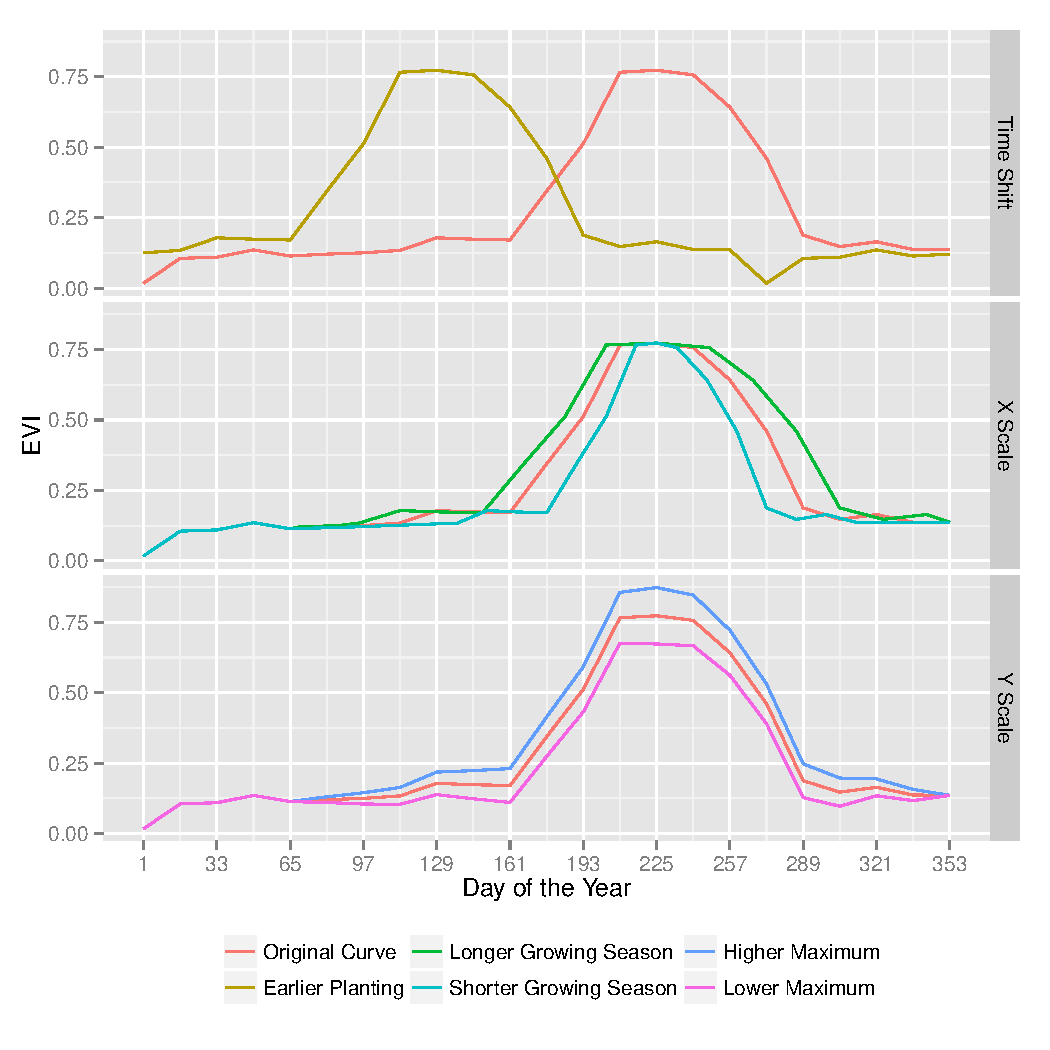
\includegraphics[width=0.7\linewidth]{Graphics/transformations.pdf}
\end{figure}
\end{frame}

\begin{frame}{TSF Method}
Two-Step Filter (TSF) method from \textcite{sakamoto2010a-two-step}
\begin{itemize}
  \item Two steps: (1) wavelet smoothing and (2) curve fitting
  \item Curve fitting can fit reference signature to unknown pixels
\end{itemize}
\end{frame}

\begin{frame}{TSF Method}
\begin{block}{TSF Equation 1}
  \begin{equation*}
    RMSE = \biggl[\frac{1}{365/s}\sum_{x\ =\ j(0),\ j(1)\ldots}^{n}\bigl(f\left(x\right)-g\left(x\right)\bigr)^{2}\biggr]^{\frac{1}{2}}
  \end{equation*}
\end{block}
\vspace{0.5\baselineskip}
where
\begin{itemize}
  \item $n$ is the number of dates in the TSI
  \item $f(x)$ is the temporal signature for a given pixel in a dataset
  \item $x$ is the DOY, as defined by $j(y)$
\end{itemize}
\end{frame}

\begin{frame}{TSF Method}
\begin{block}{TSF Equation 2}
  \begin{equation*}
    g(x) = yscale\times~h\left(xscale\times(x + tshift)\right)
  \end{equation*}
\end{block}
\vspace{0.5\baselineskip}
where
\begin{itemize}
  \item $yscale$ and  $xscale$ are coefficients controlling the vertical and horizontal scaling of a reference signature $h(x)$
  \item $tshift$ is a constant representing the horizontal shift, in days, of $h(x)$
  \item $x$ is the DOY
\end{itemize}
\end{frame}

\begin{frame}{TSF Method}
\begin{figure}
  \centering
  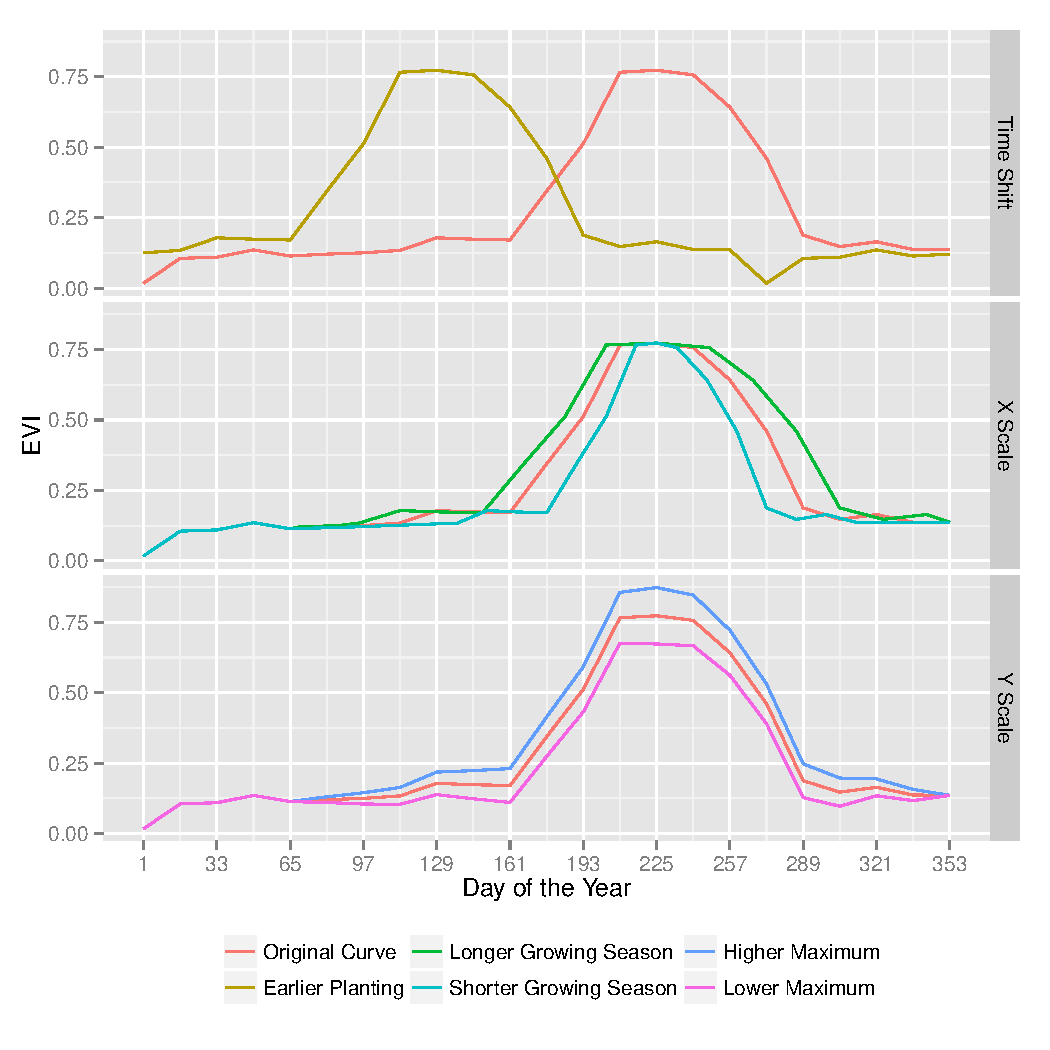
\includegraphics[width=0.7\linewidth]{Graphics/transformations.pdf}
\end{figure}
\end{frame}

\begin{frame}{TSF Method}
\begin{block}{TSF Equation 1}
  \begin{equation*}
    RMSE = \biggl[\frac{1}{365/s}\sum_{x\ =\ j(0),\ j(1)\ldots}^{n}\bigl(f\left(x\right)-g\left(x\right)\bigr)^{2}\biggr]^{\frac{1}{2}}
  \end{equation*}
\end{block}
\vspace{0.5\baselineskip}
Minimizing Equation 1 with appropriate constraints on $yscale$, $xscale$, and $tshift$ will find the fit of a a reference signature to a pixel.

\alert<2>{The signature with the lowest RMSE provides the most probable identification.}
\end{frame}

\begin{frame}{Phenological Classification}
\begin{alertblock}{Problem}
  What if you don’t have training sites?
\end{alertblock}
\visible<2->{\begin{block}{Answer}
  The TSF equations allow the classification of unknown pixels\\using a library of crop signatures.
\end{block}}
\end{frame}


% STUDY AREAS
\section{Study Areas}

\subsection{Kansas}
\begin{frame}{Kansas Study Area}
\begin{columns}[onlytextwidth]
\begin{column}{0.47\textwidth}
  \begin{itemize}
    \item 2012 Kansas top crops:
      \begin{itemize}
        \item Winter wheat
        \item Corn
        \item Soy
      \end{itemize}
    \item Ground truth:\\USDA Cropland Data Layer
  \end{itemize}
\end{column}
\begin{column}{0.53\textwidth}
  \begin{figure}
    \includegraphics[width=1.02\textwidth,right]{Graphics/KSstudysite.pdf}
  \end{figure}
\end{column}
\end{columns}
\end{frame}

\begin{frame}{Kansas Study Area}
\begin{table}
  \centering
  \caption[Kansas Study Site Planting Dates]{\parbox{2.5in}{\centering~Kansas Study Site Planting Dates \scriptsize\autocite[adapted from][]{shroyer1996kansas}}}
  \begin{tabular}{L{.75in} R{1.75in}}
    \toprule
    \Book{Crop} & \Book{Planting Date Range} \\
    \midrule
    Wheat & \datenoyear{25}{9} to \datenoyear{20}{10} \\
    Corn & \datenoyear{1}{4} to \datenoyear{10}{5} \\
    Sorghum & \datenoyear{15}{5} to \datenoyear{20}{6} \\
    Soybeans & \datenoyear{5}{5} to \datenoyear{10}{6} \\
    \bottomrule
  \end{tabular}
\end{table}

\end{frame}



\subsection{Pellegrini}
\begin{frame}{Department of Pellegrini}
  \begin{figure}
    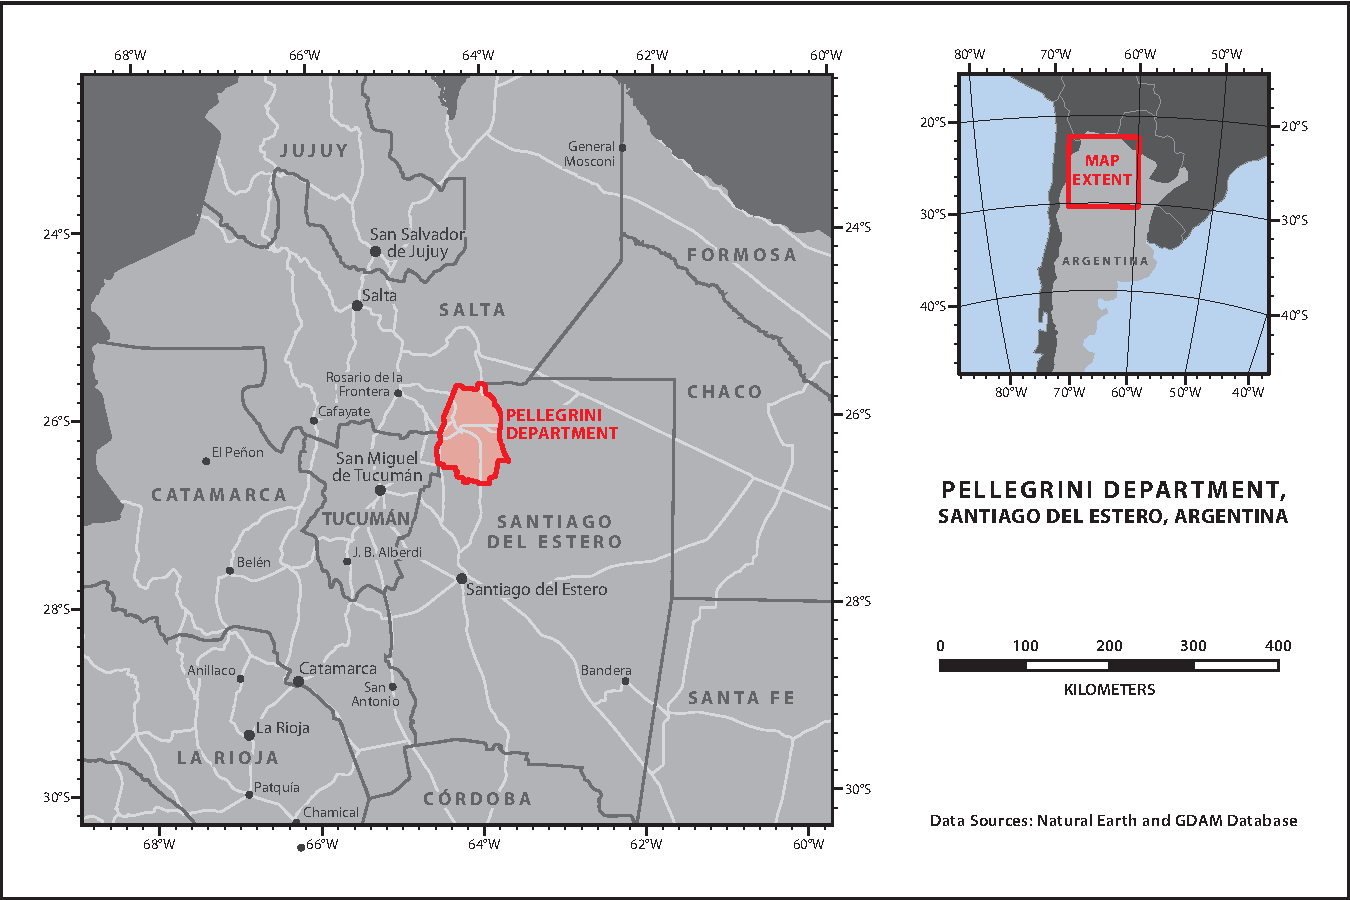
\includegraphics[width=0.97\textwidth]{Graphics/argentinaOverview_landscape.pdf}
  \end{figure}
\end{frame}

\begin{frame}{Department of Pellegrini}
  \begin{figure}
    \includegraphics[width=1.0\textwidth]{Graphics/pellegrini75to14_landscape.pdf}
  \end{figure}
\end{frame}

\begin{frame}{Department of Pellegrini}
\centering

\begin{table}
  \caption{Deforestation in Pellegrini, 2001 to 2011}
  \begin{tabular}{lSS[table-figures-decimal=1]S}  
    \toprule
    \multirow{2}{*}{\Book{Time Period}} & \multirow{2}{*}{\parbox{0.75in}{\raggedleft\Book{Hectares Cleared}}} & \multirow{2}{*}{\parbox{0.75in}{\raggedleft\Book{Percent of Land Area}}} & \multirow{2}{*}{\parbox{0.75in}{\raggedleft\Book{Hectares per Year}}} \\
     & & & \\
    \midrule
    2001 to 2005 & 5968 & 0.9 & 1492 \\
    2006 to 2011 & 75249 & 10.9 & 15050 \\
    \bottomrule
  \end{tabular}
\end{table}
\visible<2>{\vspace{\baselineskip}
\centering
\alert{Annual rate of clearing increased over 1000\%!}}
\end{frame}

\begin{frame}{Department of Pellegrini}
Top crops in Pellegrini, 2001 to 2005
\begin{itemize}
  \item Soy
  \item Corn
  \item Winter Wheat
\end{itemize}
\autocite[From][]{volante2005analisis}
\end{frame}


% DATA AND METHODS
\section{Data and Methods}

\subsection{Datasets}
\begin{frame}{Datasets}
\begin{itemize}
  \item<1-> 250-meter MODIS 16-day composite VI imagery
  \item<2-> 30-meter 2012 USDA Cropland Data Layer
  \item<3-> 30-meter Landsat 8 OLI satellite imagery
  \item<4-> Pellegrini boundary shapefile
\end{itemize}
\end{frame}

\begin{frame}{Datasets}
\begin{itemize}
  \item<1-> 2014 Pellegrini Land Cover vector dataset
\end{itemize}
\end{frame}


\subsection{Pellegrini Data Collection}
\begin{frame}{Pellegrini Data Collection}
\begin{itemize}
  \item<1-> Data collection in Pellegrini \datenoyear{12}{3} to \datenoyear{3}{4}
  \begin{itemize}
    \item<2-> 400 random sample points
    \begin{itemize}
      \item<3-> Direct observation
      \item<3-> Interviews with farmers
      \item<3-> Satellite image interpretation
    \end{itemize}
    \item<4-> Agricultural practices and planting/harvesting dates
  \end{itemize}
\end{itemize}
\end{frame}


\subsection{Data Processing}
\begin{frame}{Processing Workflow}
\begin{enumerate}
  \item Reproject the MODIS composite VIs
  \item Assemble composite VIs into TSIs
  \item Extract crop signatures from the Kansas TSI
  \begin{enumerate}
    \item Identify pure pixels (e.g. non-mixels)
    \item Use the CDL to isolate each crop
    \item Identify phenological groups using k-means clustering
    \item Extract pixel values for each group and average
  \end{enumerate}
  \item Fit the Kansas signatures to the Kansas TSI using the TSF method
  \item Classify the Kansas RMSE rasters and assess accuracy
  \item Fit the Kansas signatures to the Argentina TSI
  \item Classify the Argentina RMSE rasters and assess accuracy
\end{enumerate}
\end{frame}

\begin{frame}{1. Reprojection}
\begin{itemize}
  \item Land Processes Distributed Active Archive Center's (LPDAAC) MODIS Reprojection Tool
\end{itemize}
\end{frame}

\begin{frame}{2. Building the TSI\NoCaseChange{s}}
\begin{itemize}
  \item<1-> Python command line tool (PCLT) to stack composites
  \item<2-> Kansas TSI covered 2012 DOY 97 to 2012 DOY 273
  \item<3-> Argentina TSI covered 2014 DOY -13 to 2014 DOY 161
  \begin{itemize}
    \item<4-> Aqua DOY 105 composite used in place of DOY 113 composite
    \item<4-> DOY 129 interpolated from DOY 105 and DOY 145 composites
  \end{itemize}
\end{itemize}
\end{frame}

\begin{frame}{3. Extract crop signatures}
\begin{enumerate}
  \item[3.1] Identify pure pixels (e.g. non-mixels)
  \begin{itemize}
    % Necessary because mixels do not have pure temporal signatures
    \item<1-> Intersected MODIS pixel grid with vectorized CDL
    \item<2-> Selected all features >= 53,000 m$^2$ in area
  \end{itemize}
\end{enumerate}
\end{frame}

\begin{frame}{3. Extract crop signatures}
\begin{enumerate}
  \item[3.2] Use the CDL to isolate each crop
  \begin{itemize}
    \item<1-> Resampled CDL to MODIS grid by majority
    \item<2-> Isolated the TSI pixels for each crop
      \begin{itemize}
        \item<3-> Corn
        \item<3-> Soy
        \item<3-> Sorghum
      \end{itemize}
  \end{itemize}
\end{enumerate}
\end{frame}

\begin{frame}{3. Extract crop signatures}
\begin{enumerate}
  \item[3.3] Identify phenological groups using k-means clustering
  \begin{itemize}
    \item<1-> ENVI k-means tool
    \item<2-> Three clusters, 1.0\% change threshold, 100 iterations
  \end{itemize}
\end{enumerate}
\end{frame}

\begin{frame}{3. Extract crop signatures}
\begin{enumerate}
  \item[3.3] Extract pixel values for each group and average
  \begin{itemize}
    \item<1-> Pixels from each k-means cluster converted to points
    \item<2-> PCLT to find mean values from points
    \begin{itemize}
      \item<2-> Produces .ref signature files
    \end{itemize}
  \end{itemize}
\end{enumerate}
\visible<3->{\centering~Now we have crop signatures!}
\end{frame}

\begin{frame}{Fitting Signatures}
\begin{enumerate}
  \item[4, 6.] Fit Kansas signatures to {\footnotesize\texttt{<insert study area here>}}\\TSI using TSF method
  \begin{itemize}
    % Kansas to Kansas for testing and verification of signatures and toolset
    \item<2-> Not using the TSF's wavelet filtering
    \item<3-> PCLT to fit reference signatures to a TSI using\\TSF equations
    \begin{itemize}
      \item<3-> Creates a RMSE raster for each signature
      \item<4-> $xscale$ and $yscale$ bounds: 0.6 to 1.4
      \item<5-> $tshift$ bounds: $\pm10$ days Kansas, 120 to 140 days Argentina
    \end{itemize}
  \end{itemize}
\end{enumerate}
\end{frame}

\begin{frame}{Classifying RMSE Rasters}
\begin{enumerate}
  \item[5, 7.] Classify {\footnotesize\texttt{<insert study area here>}} RMSE rasters\\and assess accuracy
  \begin{itemize}
    \item<2-> Signature with lowest RMSE value is best identification
    \item<3-> Not all RMSE values should be considered
    \begin{itemize}
      \item<4-> If all signatures have high RMSE values,\\none are a good match
    \end{itemize}
  \end{itemize}
\end{enumerate}
\visible<5->{\begin{alertblock}{Problem}
  How do we determine which RMSE values to consider?
\end{alertblock}}
\end{frame}

\begin{frame}{Classifying RMSE Rasters}
\begin{alertblock}{Problem}
  How do we determine which RMSE values to consider?
\end{alertblock}
\visible<2->{\begin{block}{Solution\visible<3->{, kind of}}
  Brute force through different threshold combinations, classifying and assessing the accuracy to find the best result.
\end{block}}
\end{frame}

\begin{frame}{Classifying RMSE Rasters}
\begin{enumerate}
  \item[5, 7.] Classify {\footnotesize\texttt{<insert study area here>}} RMSE rasters\\and assess accuracy
  \begin{itemize}
    \item<2-> PCLT to iterate through user-defined range of thresholds
    \item<3-> Classification and accuracy rasters with best combination
  \end{itemize}
\end{enumerate}
\end{frame}


% RESULTS AND DISCUSSION
\section{Results and Discussion}
\begin{frame}{Results}
\begin{itemize}
  \item Summer 2014 Pellegrini ground truth
  \item Pellegrini agricultural practices
  \item Kansas crop signatures
  \item Kansas classification
  \item Pellegrini classification
\end{itemize}
\end{frame}

\subsection{Pellegrini Data}
\begin{frame}{Pellegrini Ground Truth}
\begin{columns}[onlytextwidth]
\begin{column}{0.47\textwidth}
  \begin{itemize}
    \item 378 of 400 sample\\points were identified
    \item Many additional\\fields were collected
  \end{itemize}
\end{column}
\begin{column}{0.53\textwidth}
  \begin{figure}
    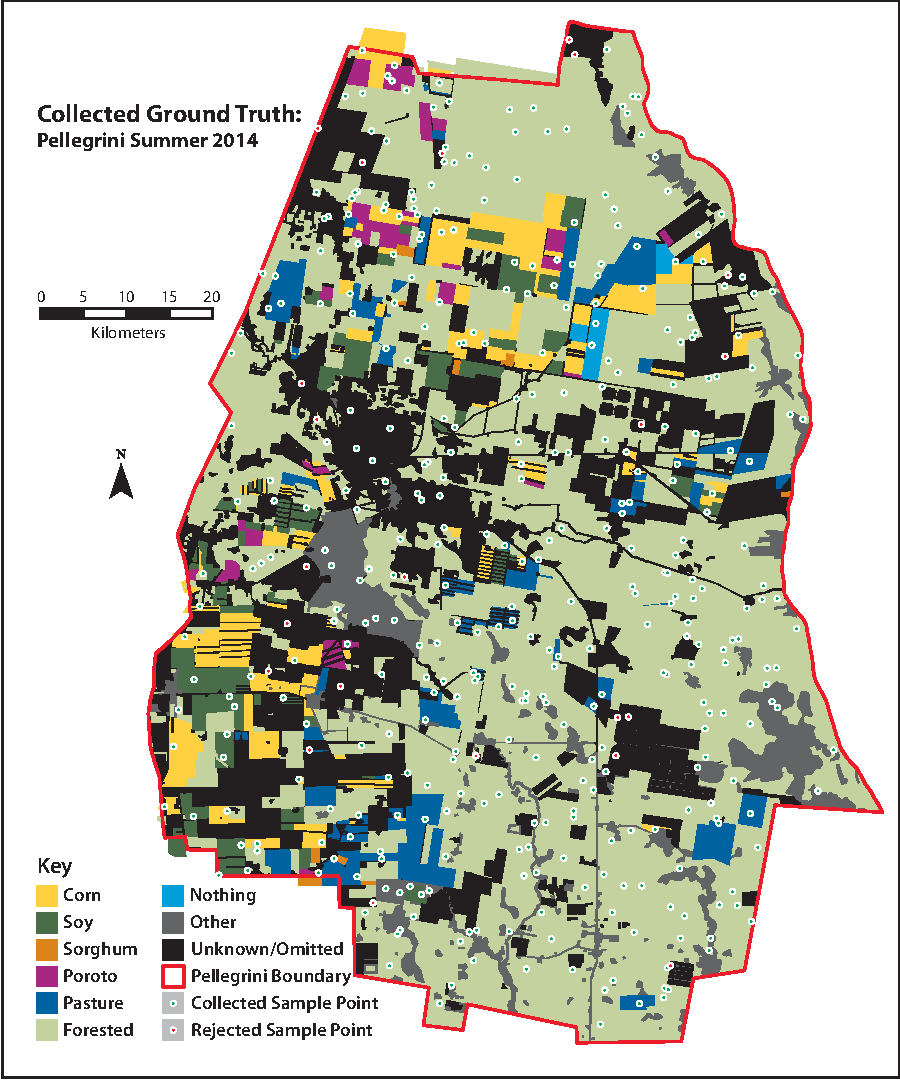
\includegraphics[width=1.0\textwidth]{Graphics/collecteddata.pdf}
  \end{figure}
\end{column}
\end{columns}
\end{frame}

\begin{frame}{Pellegrini Ground Truth}
\begin{table}
  \centering
  \caption{\parbox{4in}{\centering\Book{Summer 2014 Pellegrini Land Cover Classes}}}
  \begin{tabular}{lSS}
    \toprule
    \Book{Cover Type} & \Book{Hectares} & \Book{Sample Points} \\
    \midrule
    Forested & 389541 & 247 \\
    Other & 42229 & 22 \\
    Corn & 41488 & 36 \\
    Pasture & 35057 & 37 \\
    Soy & 27498 & 24 \\
    Poroto & 9539 & 7 \\
    Nothing & 3057 & 3 \\
    Sorghum & 1646 & 2 \\
    \midrule
    Unknown & 92248 & 17 \\
    Omitted & 52052 & 5 \\
    \midrule
    \Book{Total} & 694346 & 400 \\
    \bottomrule
  \end{tabular}
\end{table}
\end{frame}

\begin{frame}{Pellegrini Agriculture}
\begin{table}
  \centering
  \caption{Key Dates for Pellegrini Summer Crops}
  \begin{tabular}{lcc}
    \toprule
    \Book{Crop} & \Book{Ideal Planting Range} & \Book{Harvesting Begins} \\
    \midrule
    Soy & \datenoyear{15}{12} to \datenoyear{15}{1} & \datenoyear{1}{5} \\
    Corn & \datenoyear{15}{1} to \datenoyear{15}{2} & \datenoyear{1}{6} \\
    Sorghum & \datenoyear{15}{1} to \datenoyear{15}{2} & \datenoyear{1}{6} \\
    Poroto & \datenoyear{15}{1} to \datenoyear{20}{2} & \datenoyear{10}{5} \\
    \bottomrule
  \end{tabular}
\end{table}
\end{frame}


\subsection{Kansas Crop Signatures}
\begin{frame}{Kansas Crop Signatures}
\visible<2->{\begin{figure}
  \centering
  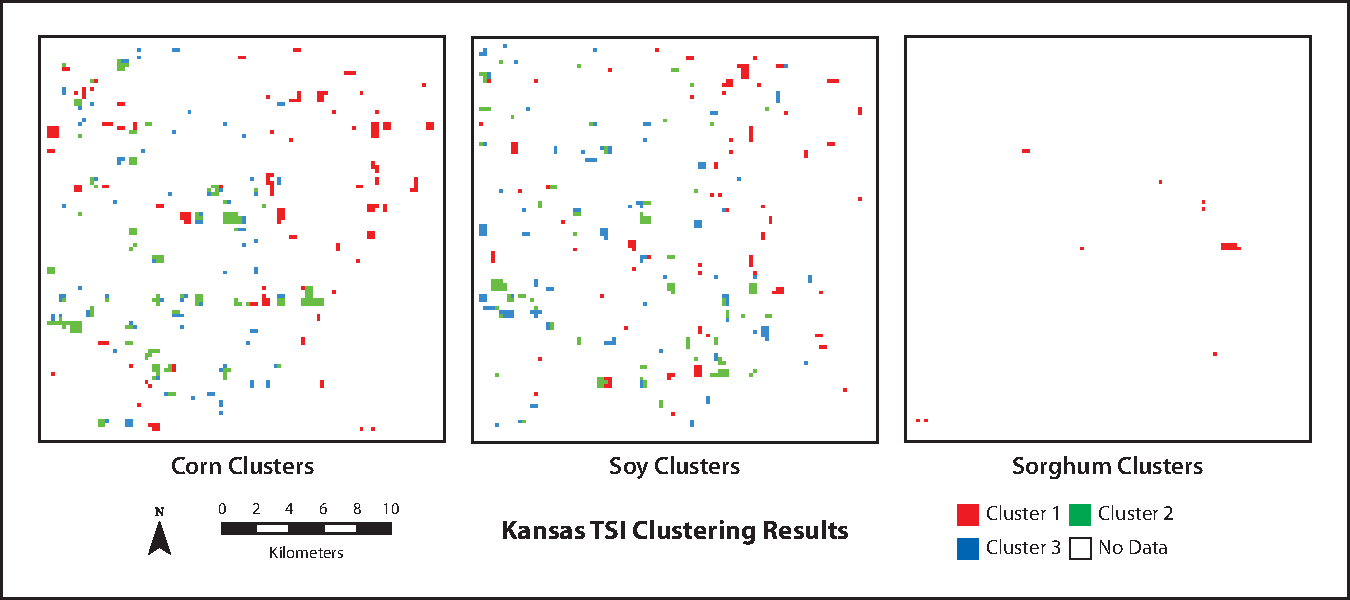
\includegraphics[width=\textwidth]{Graphics/KSclustered.pdf}
\end{figure}}
\end{frame}

\begin{frame}{Kansas Crop Signatures}
\begin{figure}
  \centering
  \resizebox{0.65\textwidth}{!}{%%Signature of ['Soy', 'Corn', 'Sorghum'] from /Users/phoetrymaster/Documents/School/Geography/Thesis/Data/MODIS_KANSAS_2007-2012/reprojected/Summer2012/kmeansTesting_2/KMEANS2_SIGS/ processed with allsigsKS.py.
%% Creator: Matplotlib, PGF backend
%%
%% To include the figure in your LaTeX document, write
%%   \input{<filename>.pgf}
%%
%% Make sure the required packages are loaded in your preamble
%%   \usepackage{pgf}
%%
%% Figures using additional raster images can only be included by \input if
%% they are in the same directory as the main LaTeX file. For loading figures
%% from other directories you can use the `import` package
%%   \usepackage{import}
%% and then include the figures with
%%   \import{<path to file>}{<filename>.pgf}
%%
%% Matplotlib used the following preamble
%%   \usepackage{fontspec}
%%   \setsansfont{Myriad Pro}
%%   \setmonofont{Bitstream Vera Sans Mono}
%%
\begingroup%
\makeatletter%
\begin{pgfpicture}%
\pgfpathrectangle{\pgfpointorigin}{\pgfqpoint{5.149972in}{5.326875in}}%
\pgfusepath{use as bounding box}%
\begin{pgfscope}%
\pgfsetbuttcap%
\pgfsetroundjoin%
\definecolor{currentfill}{rgb}{1.000000,1.000000,1.000000}%
\pgfsetfillcolor{currentfill}%
\pgfsetlinewidth{0.000000pt}%
\definecolor{currentstroke}{rgb}{1.000000,1.000000,1.000000}%
\pgfsetstrokecolor{currentstroke}%
\pgfsetdash{}{0pt}%
\pgfpathmoveto{\pgfqpoint{-0.000000in}{0.000000in}}%
\pgfpathlineto{\pgfqpoint{5.149972in}{0.000000in}}%
\pgfpathlineto{\pgfqpoint{5.149972in}{5.326875in}}%
\pgfpathlineto{\pgfqpoint{-0.000000in}{5.326875in}}%
\pgfpathclose%
\pgfusepath{fill}%
\end{pgfscope}%
\begin{pgfscope}%
\pgfsetbuttcap%
\pgfsetroundjoin%
\definecolor{currentfill}{rgb}{0.898039,0.898039,0.898039}%
\pgfsetfillcolor{currentfill}%
\pgfsetlinewidth{0.000000pt}%
\definecolor{currentstroke}{rgb}{0.000000,0.000000,0.000000}%
\pgfsetstrokecolor{currentstroke}%
\pgfsetstrokeopacity{0.000000}%
\pgfsetdash{}{0pt}%
\pgfpathmoveto{\pgfqpoint{0.593722in}{1.226875in}}%
\pgfpathlineto{\pgfqpoint{5.049972in}{1.226875in}}%
\pgfpathlineto{\pgfqpoint{5.049972in}{5.226875in}}%
\pgfpathlineto{\pgfqpoint{0.593722in}{5.226875in}}%
\pgfpathclose%
\pgfusepath{fill}%
\end{pgfscope}%
\begin{pgfscope}%
\pgfpathrectangle{\pgfqpoint{0.593722in}{1.226875in}}{\pgfqpoint{4.456250in}{4.000000in}} %
\pgfusepath{clip}%
\pgfsetroundcap%
\pgfsetroundjoin%
\pgfsetlinewidth{1.003750pt}%
\definecolor{currentstroke}{rgb}{1.000000,1.000000,1.000000}%
\pgfsetstrokecolor{currentstroke}%
\pgfsetdash{}{0pt}%
\pgfpathmoveto{\pgfqpoint{0.936511in}{1.226875in}}%
\pgfpathlineto{\pgfqpoint{0.936511in}{5.226875in}}%
\pgfusepath{stroke}%
\end{pgfscope}%
\begin{pgfscope}%
\pgfsetbuttcap%
\pgfsetroundjoin%
\definecolor{currentfill}{rgb}{0.5,0.5,0.5}%
\pgfsetfillcolor{currentfill}%
\pgfsetlinewidth{1.003750pt}%
\definecolor{currentstroke}{rgb}{0.5,0.5,0.5}%
\pgfsetstrokecolor{currentstroke}%
\pgfsetdash{}{0pt}%
\pgfsys@defobject{currentmarker}{\pgfqpoint{0.000000in}{-0.055556in}}{\pgfqpoint{0.000000in}{0.000000in}}{%
\pgfpathmoveto{\pgfqpoint{0.000000in}{0.000000in}}%
\pgfpathlineto{\pgfqpoint{0.000000in}{-0.055556in}}%
\pgfusepath{stroke,fill}%
}%
\begin{pgfscope}%
\pgfsys@transformshift{0.936511in}{1.226875in}%
\pgfsys@useobject{currentmarker}{}%
\end{pgfscope}%
\end{pgfscope}%
\begin{pgfscope}%
\definecolor{textcolor}{rgb}{0.5,0.5,0.5}%
\pgfsetstrokecolor{textcolor}%
\pgfsetfillcolor{textcolor}%
\pgftext[x=0.936511in,y=1.115763in,,top]{{\rmfamily\fontsize{10.000000}{12.000000}\selectfont\color{textcolor} 97}}%
\end{pgfscope}%
\begin{pgfscope}%
\pgfpathrectangle{\pgfqpoint{0.593722in}{1.226875in}}{\pgfqpoint{4.456250in}{4.000000in}} %
\pgfusepath{clip}%
\pgfsetroundcap%
\pgfsetroundjoin%
\pgfsetlinewidth{1.003750pt}%
\definecolor{currentstroke}{rgb}{1.000000,1.000000,1.000000}%
\pgfsetstrokecolor{currentstroke}%
\pgfsetdash{}{0pt}%
\pgfpathmoveto{\pgfqpoint{1.622087in}{1.226875in}}%
\pgfpathlineto{\pgfqpoint{1.622087in}{5.226875in}}%
\pgfusepath{stroke}%
\end{pgfscope}%
\begin{pgfscope}%
\pgfsetbuttcap%
\pgfsetroundjoin%
\definecolor{currentfill}{rgb}{0.5,0.5,0.5}%
\pgfsetfillcolor{currentfill}%
\pgfsetlinewidth{1.003750pt}%
\definecolor{currentstroke}{rgb}{0.5,0.5,0.5}%
\pgfsetstrokecolor{currentstroke}%
\pgfsetdash{}{0pt}%
\pgfsys@defobject{currentmarker}{\pgfqpoint{0.000000in}{-0.055556in}}{\pgfqpoint{0.000000in}{0.000000in}}{%
\pgfpathmoveto{\pgfqpoint{0.000000in}{0.000000in}}%
\pgfpathlineto{\pgfqpoint{0.000000in}{-0.055556in}}%
\pgfusepath{stroke,fill}%
}%
\begin{pgfscope}%
\pgfsys@transformshift{1.622087in}{1.226875in}%
\pgfsys@useobject{currentmarker}{}%
\end{pgfscope}%
\end{pgfscope}%
\begin{pgfscope}%
\definecolor{textcolor}{rgb}{0.5,0.5,0.5}%
\pgfsetstrokecolor{textcolor}%
\pgfsetfillcolor{textcolor}%
\pgftext[x=1.622087in,y=1.115763in,,top]{{\rmfamily\fontsize{10.000000}{12.000000}\selectfont\color{textcolor} 129}}%
\end{pgfscope}%
\begin{pgfscope}%
\pgfpathrectangle{\pgfqpoint{0.593722in}{1.226875in}}{\pgfqpoint{4.456250in}{4.000000in}} %
\pgfusepath{clip}%
\pgfsetroundcap%
\pgfsetroundjoin%
\pgfsetlinewidth{1.003750pt}%
\definecolor{currentstroke}{rgb}{1.000000,1.000000,1.000000}%
\pgfsetstrokecolor{currentstroke}%
\pgfsetdash{}{0pt}%
\pgfpathmoveto{\pgfqpoint{2.307664in}{1.226875in}}%
\pgfpathlineto{\pgfqpoint{2.307664in}{5.226875in}}%
\pgfusepath{stroke}%
\end{pgfscope}%
\begin{pgfscope}%
\pgfsetbuttcap%
\pgfsetroundjoin%
\definecolor{currentfill}{rgb}{0.5,0.5,0.5}%
\pgfsetfillcolor{currentfill}%
\pgfsetlinewidth{1.003750pt}%
\definecolor{currentstroke}{rgb}{0.5,0.5,0.5}%
\pgfsetstrokecolor{currentstroke}%
\pgfsetdash{}{0pt}%
\pgfsys@defobject{currentmarker}{\pgfqpoint{0.000000in}{-0.055556in}}{\pgfqpoint{0.000000in}{0.000000in}}{%
\pgfpathmoveto{\pgfqpoint{0.000000in}{0.000000in}}%
\pgfpathlineto{\pgfqpoint{0.000000in}{-0.055556in}}%
\pgfusepath{stroke,fill}%
}%
\begin{pgfscope}%
\pgfsys@transformshift{2.307664in}{1.226875in}%
\pgfsys@useobject{currentmarker}{}%
\end{pgfscope}%
\end{pgfscope}%
\begin{pgfscope}%
\definecolor{textcolor}{rgb}{0.5,0.5,0.5}%
\pgfsetstrokecolor{textcolor}%
\pgfsetfillcolor{textcolor}%
\pgftext[x=2.307664in,y=1.115763in,,top]{{\rmfamily\fontsize{10.000000}{12.000000}\selectfont\color{textcolor} 161}}%
\end{pgfscope}%
\begin{pgfscope}%
\pgfpathrectangle{\pgfqpoint{0.593722in}{1.226875in}}{\pgfqpoint{4.456250in}{4.000000in}} %
\pgfusepath{clip}%
\pgfsetroundcap%
\pgfsetroundjoin%
\pgfsetlinewidth{1.003750pt}%
\definecolor{currentstroke}{rgb}{1.000000,1.000000,1.000000}%
\pgfsetstrokecolor{currentstroke}%
\pgfsetdash{}{0pt}%
\pgfpathmoveto{\pgfqpoint{2.993241in}{1.226875in}}%
\pgfpathlineto{\pgfqpoint{2.993241in}{5.226875in}}%
\pgfusepath{stroke}%
\end{pgfscope}%
\begin{pgfscope}%
\pgfsetbuttcap%
\pgfsetroundjoin%
\definecolor{currentfill}{rgb}{0.5,0.5,0.5}%
\pgfsetfillcolor{currentfill}%
\pgfsetlinewidth{1.003750pt}%
\definecolor{currentstroke}{rgb}{0.5,0.5,0.5}%
\pgfsetstrokecolor{currentstroke}%
\pgfsetdash{}{0pt}%
\pgfsys@defobject{currentmarker}{\pgfqpoint{0.000000in}{-0.055556in}}{\pgfqpoint{0.000000in}{0.000000in}}{%
\pgfpathmoveto{\pgfqpoint{0.000000in}{0.000000in}}%
\pgfpathlineto{\pgfqpoint{0.000000in}{-0.055556in}}%
\pgfusepath{stroke,fill}%
}%
\begin{pgfscope}%
\pgfsys@transformshift{2.993241in}{1.226875in}%
\pgfsys@useobject{currentmarker}{}%
\end{pgfscope}%
\end{pgfscope}%
\begin{pgfscope}%
\definecolor{textcolor}{rgb}{0.5,0.5,0.5}%
\pgfsetstrokecolor{textcolor}%
\pgfsetfillcolor{textcolor}%
\pgftext[x=2.993241in,y=1.115763in,,top]{{\rmfamily\fontsize{10.000000}{12.000000}\selectfont\color{textcolor} 193}}%
\end{pgfscope}%
\begin{pgfscope}%
\pgfpathrectangle{\pgfqpoint{0.593722in}{1.226875in}}{\pgfqpoint{4.456250in}{4.000000in}} %
\pgfusepath{clip}%
\pgfsetroundcap%
\pgfsetroundjoin%
\pgfsetlinewidth{1.003750pt}%
\definecolor{currentstroke}{rgb}{1.000000,1.000000,1.000000}%
\pgfsetstrokecolor{currentstroke}%
\pgfsetdash{}{0pt}%
\pgfpathmoveto{\pgfqpoint{3.678818in}{1.226875in}}%
\pgfpathlineto{\pgfqpoint{3.678818in}{5.226875in}}%
\pgfusepath{stroke}%
\end{pgfscope}%
\begin{pgfscope}%
\pgfsetbuttcap%
\pgfsetroundjoin%
\definecolor{currentfill}{rgb}{0.5,0.5,0.5}%
\pgfsetfillcolor{currentfill}%
\pgfsetlinewidth{1.003750pt}%
\definecolor{currentstroke}{rgb}{0.5,0.5,0.5}%
\pgfsetstrokecolor{currentstroke}%
\pgfsetdash{}{0pt}%
\pgfsys@defobject{currentmarker}{\pgfqpoint{0.000000in}{-0.055556in}}{\pgfqpoint{0.000000in}{0.000000in}}{%
\pgfpathmoveto{\pgfqpoint{0.000000in}{0.000000in}}%
\pgfpathlineto{\pgfqpoint{0.000000in}{-0.055556in}}%
\pgfusepath{stroke,fill}%
}%
\begin{pgfscope}%
\pgfsys@transformshift{3.678818in}{1.226875in}%
\pgfsys@useobject{currentmarker}{}%
\end{pgfscope}%
\end{pgfscope}%
\begin{pgfscope}%
\definecolor{textcolor}{rgb}{0.5,0.5,0.5}%
\pgfsetstrokecolor{textcolor}%
\pgfsetfillcolor{textcolor}%
\pgftext[x=3.678818in,y=1.115763in,,top]{{\rmfamily\fontsize{10.000000}{12.000000}\selectfont\color{textcolor} 225}}%
\end{pgfscope}%
\begin{pgfscope}%
\pgfpathrectangle{\pgfqpoint{0.593722in}{1.226875in}}{\pgfqpoint{4.456250in}{4.000000in}} %
\pgfusepath{clip}%
\pgfsetroundcap%
\pgfsetroundjoin%
\pgfsetlinewidth{1.003750pt}%
\definecolor{currentstroke}{rgb}{1.000000,1.000000,1.000000}%
\pgfsetstrokecolor{currentstroke}%
\pgfsetdash{}{0pt}%
\pgfpathmoveto{\pgfqpoint{4.364395in}{1.226875in}}%
\pgfpathlineto{\pgfqpoint{4.364395in}{5.226875in}}%
\pgfusepath{stroke}%
\end{pgfscope}%
\begin{pgfscope}%
\pgfsetbuttcap%
\pgfsetroundjoin%
\definecolor{currentfill}{rgb}{0.5,0.5,0.5}%
\pgfsetfillcolor{currentfill}%
\pgfsetlinewidth{1.003750pt}%
\definecolor{currentstroke}{rgb}{0.5,0.5,0.5}%
\pgfsetstrokecolor{currentstroke}%
\pgfsetdash{}{0pt}%
\pgfsys@defobject{currentmarker}{\pgfqpoint{0.000000in}{-0.055556in}}{\pgfqpoint{0.000000in}{0.000000in}}{%
\pgfpathmoveto{\pgfqpoint{0.000000in}{0.000000in}}%
\pgfpathlineto{\pgfqpoint{0.000000in}{-0.055556in}}%
\pgfusepath{stroke,fill}%
}%
\begin{pgfscope}%
\pgfsys@transformshift{4.364395in}{1.226875in}%
\pgfsys@useobject{currentmarker}{}%
\end{pgfscope}%
\end{pgfscope}%
\begin{pgfscope}%
\definecolor{textcolor}{rgb}{0.5,0.5,0.5}%
\pgfsetstrokecolor{textcolor}%
\pgfsetfillcolor{textcolor}%
\pgftext[x=4.364395in,y=1.115763in,,top]{{\rmfamily\fontsize{10.000000}{12.000000}\selectfont\color{textcolor} 257}}%
\end{pgfscope}%
\begin{pgfscope}%
\pgfpathrectangle{\pgfqpoint{0.593722in}{1.226875in}}{\pgfqpoint{4.456250in}{4.000000in}} %
\pgfusepath{clip}%
\pgfsetroundcap%
\pgfsetroundjoin%
\pgfsetlinewidth{0.501875pt}%
\definecolor{currentstroke}{rgb}{1.000000,1.000000,1.000000}%
\pgfsetstrokecolor{currentstroke}%
\pgfsetdash{}{0pt}%
\pgfpathmoveto{\pgfqpoint{0.936511in}{1.226875in}}%
\pgfpathlineto{\pgfqpoint{0.936511in}{5.226875in}}%
\pgfusepath{stroke}%
\end{pgfscope}%
\begin{pgfscope}%
\pgfsetbuttcap%
\pgfsetroundjoin%
\definecolor{currentfill}{rgb}{0.5,0.5,0.5}%
\pgfsetfillcolor{currentfill}%
\pgfsetlinewidth{0.501875pt}%
\definecolor{currentstroke}{rgb}{0.5,0.5,0.5}%
\pgfsetstrokecolor{currentstroke}%
\pgfsetdash{}{0pt}%
\pgfsys@defobject{currentmarker}{\pgfqpoint{0.000000in}{0.000000in}}{\pgfqpoint{0.000000in}{0.000000in}}{%
\pgfpathmoveto{\pgfqpoint{0.000000in}{0.000000in}}%
\pgfpathlineto{\pgfqpoint{0.000000in}{0.000000in}}%
\pgfusepath{stroke,fill}%
}%
\begin{pgfscope}%
\pgfsys@transformshift{0.936511in}{1.226875in}%
\pgfsys@useobject{currentmarker}{}%
\end{pgfscope}%
\end{pgfscope}%
\begin{pgfscope}%
\pgfsetbuttcap%
\pgfsetroundjoin%
\definecolor{currentfill}{rgb}{0.5,0.5,0.5}%
\pgfsetfillcolor{currentfill}%
\pgfsetlinewidth{0.501875pt}%
\definecolor{currentstroke}{rgb}{0.5,0.5,0.5}%
\pgfsetstrokecolor{currentstroke}%
\pgfsetdash{}{0pt}%
\pgfsys@defobject{currentmarker}{\pgfqpoint{0.000000in}{0.000000in}}{\pgfqpoint{0.000000in}{0.000000in}}{%
\pgfpathmoveto{\pgfqpoint{0.000000in}{0.000000in}}%
\pgfpathlineto{\pgfqpoint{0.000000in}{0.000000in}}%
\pgfusepath{stroke,fill}%
}%
\begin{pgfscope}%
\pgfsys@transformshift{0.936511in}{5.226875in}%
\pgfsys@useobject{currentmarker}{}%
\end{pgfscope}%
\end{pgfscope}%
\begin{pgfscope}%
\pgfpathrectangle{\pgfqpoint{0.593722in}{1.226875in}}{\pgfqpoint{4.456250in}{4.000000in}} %
\pgfusepath{clip}%
\pgfsetroundcap%
\pgfsetroundjoin%
\pgfsetlinewidth{0.501875pt}%
\definecolor{currentstroke}{rgb}{1.000000,1.000000,1.000000}%
\pgfsetstrokecolor{currentstroke}%
\pgfsetdash{}{0pt}%
\pgfpathmoveto{\pgfqpoint{1.279299in}{1.226875in}}%
\pgfpathlineto{\pgfqpoint{1.279299in}{5.226875in}}%
\pgfusepath{stroke}%
\end{pgfscope}%
\begin{pgfscope}%
\pgfsetbuttcap%
\pgfsetroundjoin%
\definecolor{currentfill}{rgb}{0.5,0.5,0.5}%
\pgfsetfillcolor{currentfill}%
\pgfsetlinewidth{0.501875pt}%
\definecolor{currentstroke}{rgb}{0.5,0.5,0.5}%
\pgfsetstrokecolor{currentstroke}%
\pgfsetdash{}{0pt}%
\pgfsys@defobject{currentmarker}{\pgfqpoint{0.000000in}{0.000000in}}{\pgfqpoint{0.000000in}{0.000000in}}{%
\pgfpathmoveto{\pgfqpoint{0.000000in}{0.000000in}}%
\pgfpathlineto{\pgfqpoint{0.000000in}{0.000000in}}%
\pgfusepath{stroke,fill}%
}%
\begin{pgfscope}%
\pgfsys@transformshift{1.279299in}{1.226875in}%
\pgfsys@useobject{currentmarker}{}%
\end{pgfscope}%
\end{pgfscope}%
\begin{pgfscope}%
\pgfsetbuttcap%
\pgfsetroundjoin%
\definecolor{currentfill}{rgb}{0.5,0.5,0.5}%
\pgfsetfillcolor{currentfill}%
\pgfsetlinewidth{0.501875pt}%
\definecolor{currentstroke}{rgb}{0.5,0.5,0.5}%
\pgfsetstrokecolor{currentstroke}%
\pgfsetdash{}{0pt}%
\pgfsys@defobject{currentmarker}{\pgfqpoint{0.000000in}{0.000000in}}{\pgfqpoint{0.000000in}{0.000000in}}{%
\pgfpathmoveto{\pgfqpoint{0.000000in}{0.000000in}}%
\pgfpathlineto{\pgfqpoint{0.000000in}{0.000000in}}%
\pgfusepath{stroke,fill}%
}%
\begin{pgfscope}%
\pgfsys@transformshift{1.279299in}{5.226875in}%
\pgfsys@useobject{currentmarker}{}%
\end{pgfscope}%
\end{pgfscope}%
\begin{pgfscope}%
\pgfpathrectangle{\pgfqpoint{0.593722in}{1.226875in}}{\pgfqpoint{4.456250in}{4.000000in}} %
\pgfusepath{clip}%
\pgfsetroundcap%
\pgfsetroundjoin%
\pgfsetlinewidth{0.501875pt}%
\definecolor{currentstroke}{rgb}{1.000000,1.000000,1.000000}%
\pgfsetstrokecolor{currentstroke}%
\pgfsetdash{}{0pt}%
\pgfpathmoveto{\pgfqpoint{1.622087in}{1.226875in}}%
\pgfpathlineto{\pgfqpoint{1.622087in}{5.226875in}}%
\pgfusepath{stroke}%
\end{pgfscope}%
\begin{pgfscope}%
\pgfsetbuttcap%
\pgfsetroundjoin%
\definecolor{currentfill}{rgb}{0.5,0.5,0.5}%
\pgfsetfillcolor{currentfill}%
\pgfsetlinewidth{0.501875pt}%
\definecolor{currentstroke}{rgb}{0.5,0.5,0.5}%
\pgfsetstrokecolor{currentstroke}%
\pgfsetdash{}{0pt}%
\pgfsys@defobject{currentmarker}{\pgfqpoint{0.000000in}{0.000000in}}{\pgfqpoint{0.000000in}{0.000000in}}{%
\pgfpathmoveto{\pgfqpoint{0.000000in}{0.000000in}}%
\pgfpathlineto{\pgfqpoint{0.000000in}{0.000000in}}%
\pgfusepath{stroke,fill}%
}%
\begin{pgfscope}%
\pgfsys@transformshift{1.622087in}{1.226875in}%
\pgfsys@useobject{currentmarker}{}%
\end{pgfscope}%
\end{pgfscope}%
\begin{pgfscope}%
\pgfsetbuttcap%
\pgfsetroundjoin%
\definecolor{currentfill}{rgb}{0.5,0.5,0.5}%
\pgfsetfillcolor{currentfill}%
\pgfsetlinewidth{0.501875pt}%
\definecolor{currentstroke}{rgb}{0.5,0.5,0.5}%
\pgfsetstrokecolor{currentstroke}%
\pgfsetdash{}{0pt}%
\pgfsys@defobject{currentmarker}{\pgfqpoint{0.000000in}{0.000000in}}{\pgfqpoint{0.000000in}{0.000000in}}{%
\pgfpathmoveto{\pgfqpoint{0.000000in}{0.000000in}}%
\pgfpathlineto{\pgfqpoint{0.000000in}{0.000000in}}%
\pgfusepath{stroke,fill}%
}%
\begin{pgfscope}%
\pgfsys@transformshift{1.622087in}{5.226875in}%
\pgfsys@useobject{currentmarker}{}%
\end{pgfscope}%
\end{pgfscope}%
\begin{pgfscope}%
\pgfpathrectangle{\pgfqpoint{0.593722in}{1.226875in}}{\pgfqpoint{4.456250in}{4.000000in}} %
\pgfusepath{clip}%
\pgfsetroundcap%
\pgfsetroundjoin%
\pgfsetlinewidth{0.501875pt}%
\definecolor{currentstroke}{rgb}{1.000000,1.000000,1.000000}%
\pgfsetstrokecolor{currentstroke}%
\pgfsetdash{}{0pt}%
\pgfpathmoveto{\pgfqpoint{1.964876in}{1.226875in}}%
\pgfpathlineto{\pgfqpoint{1.964876in}{5.226875in}}%
\pgfusepath{stroke}%
\end{pgfscope}%
\begin{pgfscope}%
\pgfsetbuttcap%
\pgfsetroundjoin%
\definecolor{currentfill}{rgb}{0.5,0.5,0.5}%
\pgfsetfillcolor{currentfill}%
\pgfsetlinewidth{0.501875pt}%
\definecolor{currentstroke}{rgb}{0.5,0.5,0.5}%
\pgfsetstrokecolor{currentstroke}%
\pgfsetdash{}{0pt}%
\pgfsys@defobject{currentmarker}{\pgfqpoint{0.000000in}{0.000000in}}{\pgfqpoint{0.000000in}{0.000000in}}{%
\pgfpathmoveto{\pgfqpoint{0.000000in}{0.000000in}}%
\pgfpathlineto{\pgfqpoint{0.000000in}{0.000000in}}%
\pgfusepath{stroke,fill}%
}%
\begin{pgfscope}%
\pgfsys@transformshift{1.964876in}{1.226875in}%
\pgfsys@useobject{currentmarker}{}%
\end{pgfscope}%
\end{pgfscope}%
\begin{pgfscope}%
\pgfsetbuttcap%
\pgfsetroundjoin%
\definecolor{currentfill}{rgb}{0.5,0.5,0.5}%
\pgfsetfillcolor{currentfill}%
\pgfsetlinewidth{0.501875pt}%
\definecolor{currentstroke}{rgb}{0.5,0.5,0.5}%
\pgfsetstrokecolor{currentstroke}%
\pgfsetdash{}{0pt}%
\pgfsys@defobject{currentmarker}{\pgfqpoint{0.000000in}{0.000000in}}{\pgfqpoint{0.000000in}{0.000000in}}{%
\pgfpathmoveto{\pgfqpoint{0.000000in}{0.000000in}}%
\pgfpathlineto{\pgfqpoint{0.000000in}{0.000000in}}%
\pgfusepath{stroke,fill}%
}%
\begin{pgfscope}%
\pgfsys@transformshift{1.964876in}{5.226875in}%
\pgfsys@useobject{currentmarker}{}%
\end{pgfscope}%
\end{pgfscope}%
\begin{pgfscope}%
\pgfpathrectangle{\pgfqpoint{0.593722in}{1.226875in}}{\pgfqpoint{4.456250in}{4.000000in}} %
\pgfusepath{clip}%
\pgfsetroundcap%
\pgfsetroundjoin%
\pgfsetlinewidth{0.501875pt}%
\definecolor{currentstroke}{rgb}{1.000000,1.000000,1.000000}%
\pgfsetstrokecolor{currentstroke}%
\pgfsetdash{}{0pt}%
\pgfpathmoveto{\pgfqpoint{2.307664in}{1.226875in}}%
\pgfpathlineto{\pgfqpoint{2.307664in}{5.226875in}}%
\pgfusepath{stroke}%
\end{pgfscope}%
\begin{pgfscope}%
\pgfsetbuttcap%
\pgfsetroundjoin%
\definecolor{currentfill}{rgb}{0.5,0.5,0.5}%
\pgfsetfillcolor{currentfill}%
\pgfsetlinewidth{0.501875pt}%
\definecolor{currentstroke}{rgb}{0.5,0.5,0.5}%
\pgfsetstrokecolor{currentstroke}%
\pgfsetdash{}{0pt}%
\pgfsys@defobject{currentmarker}{\pgfqpoint{0.000000in}{0.000000in}}{\pgfqpoint{0.000000in}{0.000000in}}{%
\pgfpathmoveto{\pgfqpoint{0.000000in}{0.000000in}}%
\pgfpathlineto{\pgfqpoint{0.000000in}{0.000000in}}%
\pgfusepath{stroke,fill}%
}%
\begin{pgfscope}%
\pgfsys@transformshift{2.307664in}{1.226875in}%
\pgfsys@useobject{currentmarker}{}%
\end{pgfscope}%
\end{pgfscope}%
\begin{pgfscope}%
\pgfsetbuttcap%
\pgfsetroundjoin%
\definecolor{currentfill}{rgb}{0.5,0.5,0.5}%
\pgfsetfillcolor{currentfill}%
\pgfsetlinewidth{0.501875pt}%
\definecolor{currentstroke}{rgb}{0.5,0.5,0.5}%
\pgfsetstrokecolor{currentstroke}%
\pgfsetdash{}{0pt}%
\pgfsys@defobject{currentmarker}{\pgfqpoint{0.000000in}{0.000000in}}{\pgfqpoint{0.000000in}{0.000000in}}{%
\pgfpathmoveto{\pgfqpoint{0.000000in}{0.000000in}}%
\pgfpathlineto{\pgfqpoint{0.000000in}{0.000000in}}%
\pgfusepath{stroke,fill}%
}%
\begin{pgfscope}%
\pgfsys@transformshift{2.307664in}{5.226875in}%
\pgfsys@useobject{currentmarker}{}%
\end{pgfscope}%
\end{pgfscope}%
\begin{pgfscope}%
\pgfpathrectangle{\pgfqpoint{0.593722in}{1.226875in}}{\pgfqpoint{4.456250in}{4.000000in}} %
\pgfusepath{clip}%
\pgfsetroundcap%
\pgfsetroundjoin%
\pgfsetlinewidth{0.501875pt}%
\definecolor{currentstroke}{rgb}{1.000000,1.000000,1.000000}%
\pgfsetstrokecolor{currentstroke}%
\pgfsetdash{}{0pt}%
\pgfpathmoveto{\pgfqpoint{2.650453in}{1.226875in}}%
\pgfpathlineto{\pgfqpoint{2.650453in}{5.226875in}}%
\pgfusepath{stroke}%
\end{pgfscope}%
\begin{pgfscope}%
\pgfsetbuttcap%
\pgfsetroundjoin%
\definecolor{currentfill}{rgb}{0.5,0.5,0.5}%
\pgfsetfillcolor{currentfill}%
\pgfsetlinewidth{0.501875pt}%
\definecolor{currentstroke}{rgb}{0.5,0.5,0.5}%
\pgfsetstrokecolor{currentstroke}%
\pgfsetdash{}{0pt}%
\pgfsys@defobject{currentmarker}{\pgfqpoint{0.000000in}{0.000000in}}{\pgfqpoint{0.000000in}{0.000000in}}{%
\pgfpathmoveto{\pgfqpoint{0.000000in}{0.000000in}}%
\pgfpathlineto{\pgfqpoint{0.000000in}{0.000000in}}%
\pgfusepath{stroke,fill}%
}%
\begin{pgfscope}%
\pgfsys@transformshift{2.650453in}{1.226875in}%
\pgfsys@useobject{currentmarker}{}%
\end{pgfscope}%
\end{pgfscope}%
\begin{pgfscope}%
\pgfsetbuttcap%
\pgfsetroundjoin%
\definecolor{currentfill}{rgb}{0.5,0.5,0.5}%
\pgfsetfillcolor{currentfill}%
\pgfsetlinewidth{0.501875pt}%
\definecolor{currentstroke}{rgb}{0.5,0.5,0.5}%
\pgfsetstrokecolor{currentstroke}%
\pgfsetdash{}{0pt}%
\pgfsys@defobject{currentmarker}{\pgfqpoint{0.000000in}{0.000000in}}{\pgfqpoint{0.000000in}{0.000000in}}{%
\pgfpathmoveto{\pgfqpoint{0.000000in}{0.000000in}}%
\pgfpathlineto{\pgfqpoint{0.000000in}{0.000000in}}%
\pgfusepath{stroke,fill}%
}%
\begin{pgfscope}%
\pgfsys@transformshift{2.650453in}{5.226875in}%
\pgfsys@useobject{currentmarker}{}%
\end{pgfscope}%
\end{pgfscope}%
\begin{pgfscope}%
\pgfpathrectangle{\pgfqpoint{0.593722in}{1.226875in}}{\pgfqpoint{4.456250in}{4.000000in}} %
\pgfusepath{clip}%
\pgfsetroundcap%
\pgfsetroundjoin%
\pgfsetlinewidth{0.501875pt}%
\definecolor{currentstroke}{rgb}{1.000000,1.000000,1.000000}%
\pgfsetstrokecolor{currentstroke}%
\pgfsetdash{}{0pt}%
\pgfpathmoveto{\pgfqpoint{2.993241in}{1.226875in}}%
\pgfpathlineto{\pgfqpoint{2.993241in}{5.226875in}}%
\pgfusepath{stroke}%
\end{pgfscope}%
\begin{pgfscope}%
\pgfsetbuttcap%
\pgfsetroundjoin%
\definecolor{currentfill}{rgb}{0.5,0.5,0.5}%
\pgfsetfillcolor{currentfill}%
\pgfsetlinewidth{0.501875pt}%
\definecolor{currentstroke}{rgb}{0.5,0.5,0.5}%
\pgfsetstrokecolor{currentstroke}%
\pgfsetdash{}{0pt}%
\pgfsys@defobject{currentmarker}{\pgfqpoint{0.000000in}{0.000000in}}{\pgfqpoint{0.000000in}{0.000000in}}{%
\pgfpathmoveto{\pgfqpoint{0.000000in}{0.000000in}}%
\pgfpathlineto{\pgfqpoint{0.000000in}{0.000000in}}%
\pgfusepath{stroke,fill}%
}%
\begin{pgfscope}%
\pgfsys@transformshift{2.993241in}{1.226875in}%
\pgfsys@useobject{currentmarker}{}%
\end{pgfscope}%
\end{pgfscope}%
\begin{pgfscope}%
\pgfsetbuttcap%
\pgfsetroundjoin%
\definecolor{currentfill}{rgb}{0.5,0.5,0.5}%
\pgfsetfillcolor{currentfill}%
\pgfsetlinewidth{0.501875pt}%
\definecolor{currentstroke}{rgb}{0.5,0.5,0.5}%
\pgfsetstrokecolor{currentstroke}%
\pgfsetdash{}{0pt}%
\pgfsys@defobject{currentmarker}{\pgfqpoint{0.000000in}{0.000000in}}{\pgfqpoint{0.000000in}{0.000000in}}{%
\pgfpathmoveto{\pgfqpoint{0.000000in}{0.000000in}}%
\pgfpathlineto{\pgfqpoint{0.000000in}{0.000000in}}%
\pgfusepath{stroke,fill}%
}%
\begin{pgfscope}%
\pgfsys@transformshift{2.993241in}{5.226875in}%
\pgfsys@useobject{currentmarker}{}%
\end{pgfscope}%
\end{pgfscope}%
\begin{pgfscope}%
\pgfpathrectangle{\pgfqpoint{0.593722in}{1.226875in}}{\pgfqpoint{4.456250in}{4.000000in}} %
\pgfusepath{clip}%
\pgfsetroundcap%
\pgfsetroundjoin%
\pgfsetlinewidth{0.501875pt}%
\definecolor{currentstroke}{rgb}{1.000000,1.000000,1.000000}%
\pgfsetstrokecolor{currentstroke}%
\pgfsetdash{}{0pt}%
\pgfpathmoveto{\pgfqpoint{3.336030in}{1.226875in}}%
\pgfpathlineto{\pgfqpoint{3.336030in}{5.226875in}}%
\pgfusepath{stroke}%
\end{pgfscope}%
\begin{pgfscope}%
\pgfsetbuttcap%
\pgfsetroundjoin%
\definecolor{currentfill}{rgb}{0.5,0.5,0.5}%
\pgfsetfillcolor{currentfill}%
\pgfsetlinewidth{0.501875pt}%
\definecolor{currentstroke}{rgb}{0.5,0.5,0.5}%
\pgfsetstrokecolor{currentstroke}%
\pgfsetdash{}{0pt}%
\pgfsys@defobject{currentmarker}{\pgfqpoint{0.000000in}{0.000000in}}{\pgfqpoint{0.000000in}{0.000000in}}{%
\pgfpathmoveto{\pgfqpoint{0.000000in}{0.000000in}}%
\pgfpathlineto{\pgfqpoint{0.000000in}{0.000000in}}%
\pgfusepath{stroke,fill}%
}%
\begin{pgfscope}%
\pgfsys@transformshift{3.336030in}{1.226875in}%
\pgfsys@useobject{currentmarker}{}%
\end{pgfscope}%
\end{pgfscope}%
\begin{pgfscope}%
\pgfsetbuttcap%
\pgfsetroundjoin%
\definecolor{currentfill}{rgb}{0.5,0.5,0.5}%
\pgfsetfillcolor{currentfill}%
\pgfsetlinewidth{0.501875pt}%
\definecolor{currentstroke}{rgb}{0.5,0.5,0.5}%
\pgfsetstrokecolor{currentstroke}%
\pgfsetdash{}{0pt}%
\pgfsys@defobject{currentmarker}{\pgfqpoint{0.000000in}{0.000000in}}{\pgfqpoint{0.000000in}{0.000000in}}{%
\pgfpathmoveto{\pgfqpoint{0.000000in}{0.000000in}}%
\pgfpathlineto{\pgfqpoint{0.000000in}{0.000000in}}%
\pgfusepath{stroke,fill}%
}%
\begin{pgfscope}%
\pgfsys@transformshift{3.336030in}{5.226875in}%
\pgfsys@useobject{currentmarker}{}%
\end{pgfscope}%
\end{pgfscope}%
\begin{pgfscope}%
\pgfpathrectangle{\pgfqpoint{0.593722in}{1.226875in}}{\pgfqpoint{4.456250in}{4.000000in}} %
\pgfusepath{clip}%
\pgfsetroundcap%
\pgfsetroundjoin%
\pgfsetlinewidth{0.501875pt}%
\definecolor{currentstroke}{rgb}{1.000000,1.000000,1.000000}%
\pgfsetstrokecolor{currentstroke}%
\pgfsetdash{}{0pt}%
\pgfpathmoveto{\pgfqpoint{3.678818in}{1.226875in}}%
\pgfpathlineto{\pgfqpoint{3.678818in}{5.226875in}}%
\pgfusepath{stroke}%
\end{pgfscope}%
\begin{pgfscope}%
\pgfsetbuttcap%
\pgfsetroundjoin%
\definecolor{currentfill}{rgb}{0.5,0.5,0.5}%
\pgfsetfillcolor{currentfill}%
\pgfsetlinewidth{0.501875pt}%
\definecolor{currentstroke}{rgb}{0.5,0.5,0.5}%
\pgfsetstrokecolor{currentstroke}%
\pgfsetdash{}{0pt}%
\pgfsys@defobject{currentmarker}{\pgfqpoint{0.000000in}{0.000000in}}{\pgfqpoint{0.000000in}{0.000000in}}{%
\pgfpathmoveto{\pgfqpoint{0.000000in}{0.000000in}}%
\pgfpathlineto{\pgfqpoint{0.000000in}{0.000000in}}%
\pgfusepath{stroke,fill}%
}%
\begin{pgfscope}%
\pgfsys@transformshift{3.678818in}{1.226875in}%
\pgfsys@useobject{currentmarker}{}%
\end{pgfscope}%
\end{pgfscope}%
\begin{pgfscope}%
\pgfsetbuttcap%
\pgfsetroundjoin%
\definecolor{currentfill}{rgb}{0.5,0.5,0.5}%
\pgfsetfillcolor{currentfill}%
\pgfsetlinewidth{0.501875pt}%
\definecolor{currentstroke}{rgb}{0.5,0.5,0.5}%
\pgfsetstrokecolor{currentstroke}%
\pgfsetdash{}{0pt}%
\pgfsys@defobject{currentmarker}{\pgfqpoint{0.000000in}{0.000000in}}{\pgfqpoint{0.000000in}{0.000000in}}{%
\pgfpathmoveto{\pgfqpoint{0.000000in}{0.000000in}}%
\pgfpathlineto{\pgfqpoint{0.000000in}{0.000000in}}%
\pgfusepath{stroke,fill}%
}%
\begin{pgfscope}%
\pgfsys@transformshift{3.678818in}{5.226875in}%
\pgfsys@useobject{currentmarker}{}%
\end{pgfscope}%
\end{pgfscope}%
\begin{pgfscope}%
\pgfpathrectangle{\pgfqpoint{0.593722in}{1.226875in}}{\pgfqpoint{4.456250in}{4.000000in}} %
\pgfusepath{clip}%
\pgfsetroundcap%
\pgfsetroundjoin%
\pgfsetlinewidth{0.501875pt}%
\definecolor{currentstroke}{rgb}{1.000000,1.000000,1.000000}%
\pgfsetstrokecolor{currentstroke}%
\pgfsetdash{}{0pt}%
\pgfpathmoveto{\pgfqpoint{4.021607in}{1.226875in}}%
\pgfpathlineto{\pgfqpoint{4.021607in}{5.226875in}}%
\pgfusepath{stroke}%
\end{pgfscope}%
\begin{pgfscope}%
\pgfsetbuttcap%
\pgfsetroundjoin%
\definecolor{currentfill}{rgb}{0.5,0.5,0.5}%
\pgfsetfillcolor{currentfill}%
\pgfsetlinewidth{0.501875pt}%
\definecolor{currentstroke}{rgb}{0.5,0.5,0.5}%
\pgfsetstrokecolor{currentstroke}%
\pgfsetdash{}{0pt}%
\pgfsys@defobject{currentmarker}{\pgfqpoint{0.000000in}{0.000000in}}{\pgfqpoint{0.000000in}{0.000000in}}{%
\pgfpathmoveto{\pgfqpoint{0.000000in}{0.000000in}}%
\pgfpathlineto{\pgfqpoint{0.000000in}{0.000000in}}%
\pgfusepath{stroke,fill}%
}%
\begin{pgfscope}%
\pgfsys@transformshift{4.021607in}{1.226875in}%
\pgfsys@useobject{currentmarker}{}%
\end{pgfscope}%
\end{pgfscope}%
\begin{pgfscope}%
\pgfsetbuttcap%
\pgfsetroundjoin%
\definecolor{currentfill}{rgb}{0.5,0.5,0.5}%
\pgfsetfillcolor{currentfill}%
\pgfsetlinewidth{0.501875pt}%
\definecolor{currentstroke}{rgb}{0.5,0.5,0.5}%
\pgfsetstrokecolor{currentstroke}%
\pgfsetdash{}{0pt}%
\pgfsys@defobject{currentmarker}{\pgfqpoint{0.000000in}{0.000000in}}{\pgfqpoint{0.000000in}{0.000000in}}{%
\pgfpathmoveto{\pgfqpoint{0.000000in}{0.000000in}}%
\pgfpathlineto{\pgfqpoint{0.000000in}{0.000000in}}%
\pgfusepath{stroke,fill}%
}%
\begin{pgfscope}%
\pgfsys@transformshift{4.021607in}{5.226875in}%
\pgfsys@useobject{currentmarker}{}%
\end{pgfscope}%
\end{pgfscope}%
\begin{pgfscope}%
\pgfpathrectangle{\pgfqpoint{0.593722in}{1.226875in}}{\pgfqpoint{4.456250in}{4.000000in}} %
\pgfusepath{clip}%
\pgfsetroundcap%
\pgfsetroundjoin%
\pgfsetlinewidth{0.501875pt}%
\definecolor{currentstroke}{rgb}{1.000000,1.000000,1.000000}%
\pgfsetstrokecolor{currentstroke}%
\pgfsetdash{}{0pt}%
\pgfpathmoveto{\pgfqpoint{4.364395in}{1.226875in}}%
\pgfpathlineto{\pgfqpoint{4.364395in}{5.226875in}}%
\pgfusepath{stroke}%
\end{pgfscope}%
\begin{pgfscope}%
\pgfsetbuttcap%
\pgfsetroundjoin%
\definecolor{currentfill}{rgb}{0.5,0.5,0.5}%
\pgfsetfillcolor{currentfill}%
\pgfsetlinewidth{0.501875pt}%
\definecolor{currentstroke}{rgb}{0.5,0.5,0.5}%
\pgfsetstrokecolor{currentstroke}%
\pgfsetdash{}{0pt}%
\pgfsys@defobject{currentmarker}{\pgfqpoint{0.000000in}{0.000000in}}{\pgfqpoint{0.000000in}{0.000000in}}{%
\pgfpathmoveto{\pgfqpoint{0.000000in}{0.000000in}}%
\pgfpathlineto{\pgfqpoint{0.000000in}{0.000000in}}%
\pgfusepath{stroke,fill}%
}%
\begin{pgfscope}%
\pgfsys@transformshift{4.364395in}{1.226875in}%
\pgfsys@useobject{currentmarker}{}%
\end{pgfscope}%
\end{pgfscope}%
\begin{pgfscope}%
\pgfsetbuttcap%
\pgfsetroundjoin%
\definecolor{currentfill}{rgb}{0.5,0.5,0.5}%
\pgfsetfillcolor{currentfill}%
\pgfsetlinewidth{0.501875pt}%
\definecolor{currentstroke}{rgb}{0.5,0.5,0.5}%
\pgfsetstrokecolor{currentstroke}%
\pgfsetdash{}{0pt}%
\pgfsys@defobject{currentmarker}{\pgfqpoint{0.000000in}{0.000000in}}{\pgfqpoint{0.000000in}{0.000000in}}{%
\pgfpathmoveto{\pgfqpoint{0.000000in}{0.000000in}}%
\pgfpathlineto{\pgfqpoint{0.000000in}{0.000000in}}%
\pgfusepath{stroke,fill}%
}%
\begin{pgfscope}%
\pgfsys@transformshift{4.364395in}{5.226875in}%
\pgfsys@useobject{currentmarker}{}%
\end{pgfscope}%
\end{pgfscope}%
\begin{pgfscope}%
\pgfpathrectangle{\pgfqpoint{0.593722in}{1.226875in}}{\pgfqpoint{4.456250in}{4.000000in}} %
\pgfusepath{clip}%
\pgfsetroundcap%
\pgfsetroundjoin%
\pgfsetlinewidth{0.501875pt}%
\definecolor{currentstroke}{rgb}{1.000000,1.000000,1.000000}%
\pgfsetstrokecolor{currentstroke}%
\pgfsetdash{}{0pt}%
\pgfpathmoveto{\pgfqpoint{4.707184in}{1.226875in}}%
\pgfpathlineto{\pgfqpoint{4.707184in}{5.226875in}}%
\pgfusepath{stroke}%
\end{pgfscope}%
\begin{pgfscope}%
\pgfsetbuttcap%
\pgfsetroundjoin%
\definecolor{currentfill}{rgb}{0.5,0.5,0.5}%
\pgfsetfillcolor{currentfill}%
\pgfsetlinewidth{0.501875pt}%
\definecolor{currentstroke}{rgb}{0.5,0.5,0.5}%
\pgfsetstrokecolor{currentstroke}%
\pgfsetdash{}{0pt}%
\pgfsys@defobject{currentmarker}{\pgfqpoint{0.000000in}{0.000000in}}{\pgfqpoint{0.000000in}{0.000000in}}{%
\pgfpathmoveto{\pgfqpoint{0.000000in}{0.000000in}}%
\pgfpathlineto{\pgfqpoint{0.000000in}{0.000000in}}%
\pgfusepath{stroke,fill}%
}%
\begin{pgfscope}%
\pgfsys@transformshift{4.707184in}{1.226875in}%
\pgfsys@useobject{currentmarker}{}%
\end{pgfscope}%
\end{pgfscope}%
\begin{pgfscope}%
\pgfsetbuttcap%
\pgfsetroundjoin%
\definecolor{currentfill}{rgb}{0.5,0.5,0.5}%
\pgfsetfillcolor{currentfill}%
\pgfsetlinewidth{0.501875pt}%
\definecolor{currentstroke}{rgb}{0.5,0.5,0.5}%
\pgfsetstrokecolor{currentstroke}%
\pgfsetdash{}{0pt}%
\pgfsys@defobject{currentmarker}{\pgfqpoint{0.000000in}{0.000000in}}{\pgfqpoint{0.000000in}{0.000000in}}{%
\pgfpathmoveto{\pgfqpoint{0.000000in}{0.000000in}}%
\pgfpathlineto{\pgfqpoint{0.000000in}{0.000000in}}%
\pgfusepath{stroke,fill}%
}%
\begin{pgfscope}%
\pgfsys@transformshift{4.707184in}{5.226875in}%
\pgfsys@useobject{currentmarker}{}%
\end{pgfscope}%
\end{pgfscope}%
\begin{pgfscope}%
\definecolor{textcolor}{rgb}{0.5,0.5,0.5}%
\pgfsetstrokecolor{textcolor}%
\pgfsetfillcolor{textcolor}%
\pgftext[x=2.821847in,y=0.922986in,,top]{{\rmfamily\fontsize{11.000000}{13.200000}\selectfont Day of Year}}%
\end{pgfscope}%
\begin{pgfscope}%
\pgfpathrectangle{\pgfqpoint{0.593722in}{1.226875in}}{\pgfqpoint{4.456250in}{4.000000in}} %
\pgfusepath{clip}%
\pgfsetroundcap%
\pgfsetroundjoin%
\pgfsetlinewidth{1.003750pt}%
\definecolor{currentstroke}{rgb}{1.000000,1.000000,1.000000}%
\pgfsetstrokecolor{currentstroke}%
\pgfsetdash{}{0pt}%
\pgfpathmoveto{\pgfqpoint{0.593722in}{1.322113in}}%
\pgfpathlineto{\pgfqpoint{5.049972in}{1.322113in}}%
\pgfusepath{stroke}%
\end{pgfscope}%
\begin{pgfscope}%
\pgfsetbuttcap%
\pgfsetroundjoin%
\definecolor{currentfill}{rgb}{0.5,0.5,0.5}%
\pgfsetfillcolor{currentfill}%
\pgfsetlinewidth{1.003750pt}%
\definecolor{currentstroke}{rgb}{0.5,0.5,0.5}%
\pgfsetstrokecolor{currentstroke}%
\pgfsetdash{}{0pt}%
\pgfsys@defobject{currentmarker}{\pgfqpoint{-0.055556in}{0.000000in}}{\pgfqpoint{0.000000in}{0.000000in}}{%
\pgfpathmoveto{\pgfqpoint{0.000000in}{0.000000in}}%
\pgfpathlineto{\pgfqpoint{-0.055556in}{0.000000in}}%
\pgfusepath{stroke,fill}%
}%
\begin{pgfscope}%
\pgfsys@transformshift{0.593722in}{1.322113in}%
\pgfsys@useobject{currentmarker}{}%
\end{pgfscope}%
\end{pgfscope}%
\begin{pgfscope}%
\definecolor{textcolor}{rgb}{0.5,0.5,0.5}%
\pgfsetstrokecolor{textcolor}%
\pgfsetfillcolor{textcolor}%
\pgftext[x=0.482611in,y=1.322113in,right,]{{\rmfamily\fontsize{10.000000}{12.000000}\selectfont\color{textcolor} 0.0}}%
\end{pgfscope}%
\begin{pgfscope}%
\pgfpathrectangle{\pgfqpoint{0.593722in}{1.226875in}}{\pgfqpoint{4.456250in}{4.000000in}} %
\pgfusepath{clip}%
\pgfsetroundcap%
\pgfsetroundjoin%
\pgfsetlinewidth{1.003750pt}%
\definecolor{currentstroke}{rgb}{1.000000,1.000000,1.000000}%
\pgfsetstrokecolor{currentstroke}%
\pgfsetdash{}{0pt}%
\pgfpathmoveto{\pgfqpoint{0.593722in}{2.084017in}}%
\pgfpathlineto{\pgfqpoint{5.049972in}{2.084017in}}%
\pgfusepath{stroke}%
\end{pgfscope}%
\begin{pgfscope}%
\pgfsetbuttcap%
\pgfsetroundjoin%
\definecolor{currentfill}{rgb}{0.5,0.5,0.5}%
\pgfsetfillcolor{currentfill}%
\pgfsetlinewidth{1.003750pt}%
\definecolor{currentstroke}{rgb}{0.5,0.5,0.5}%
\pgfsetstrokecolor{currentstroke}%
\pgfsetdash{}{0pt}%
\pgfsys@defobject{currentmarker}{\pgfqpoint{-0.055556in}{0.000000in}}{\pgfqpoint{0.000000in}{0.000000in}}{%
\pgfpathmoveto{\pgfqpoint{0.000000in}{0.000000in}}%
\pgfpathlineto{\pgfqpoint{-0.055556in}{0.000000in}}%
\pgfusepath{stroke,fill}%
}%
\begin{pgfscope}%
\pgfsys@transformshift{0.593722in}{2.084017in}%
\pgfsys@useobject{currentmarker}{}%
\end{pgfscope}%
\end{pgfscope}%
\begin{pgfscope}%
\definecolor{textcolor}{rgb}{0.5,0.5,0.5}%
\pgfsetstrokecolor{textcolor}%
\pgfsetfillcolor{textcolor}%
\pgftext[x=0.482611in,y=2.084017in,right,]{{\rmfamily\fontsize{10.000000}{12.000000}\selectfont\color{textcolor} 0.2}}%
\end{pgfscope}%
\begin{pgfscope}%
\pgfpathrectangle{\pgfqpoint{0.593722in}{1.226875in}}{\pgfqpoint{4.456250in}{4.000000in}} %
\pgfusepath{clip}%
\pgfsetroundcap%
\pgfsetroundjoin%
\pgfsetlinewidth{1.003750pt}%
\definecolor{currentstroke}{rgb}{1.000000,1.000000,1.000000}%
\pgfsetstrokecolor{currentstroke}%
\pgfsetdash{}{0pt}%
\pgfpathmoveto{\pgfqpoint{0.593722in}{2.845922in}}%
\pgfpathlineto{\pgfqpoint{5.049972in}{2.845922in}}%
\pgfusepath{stroke}%
\end{pgfscope}%
\begin{pgfscope}%
\pgfsetbuttcap%
\pgfsetroundjoin%
\definecolor{currentfill}{rgb}{0.5,0.5,0.5}%
\pgfsetfillcolor{currentfill}%
\pgfsetlinewidth{1.003750pt}%
\definecolor{currentstroke}{rgb}{0.5,0.5,0.5}%
\pgfsetstrokecolor{currentstroke}%
\pgfsetdash{}{0pt}%
\pgfsys@defobject{currentmarker}{\pgfqpoint{-0.055556in}{0.000000in}}{\pgfqpoint{0.000000in}{0.000000in}}{%
\pgfpathmoveto{\pgfqpoint{0.000000in}{0.000000in}}%
\pgfpathlineto{\pgfqpoint{-0.055556in}{0.000000in}}%
\pgfusepath{stroke,fill}%
}%
\begin{pgfscope}%
\pgfsys@transformshift{0.593722in}{2.845922in}%
\pgfsys@useobject{currentmarker}{}%
\end{pgfscope}%
\end{pgfscope}%
\begin{pgfscope}%
\definecolor{textcolor}{rgb}{0.5,0.5,0.5}%
\pgfsetstrokecolor{textcolor}%
\pgfsetfillcolor{textcolor}%
\pgftext[x=0.482611in,y=2.845922in,right,]{{\rmfamily\fontsize{10.000000}{12.000000}\selectfont\color{textcolor} 0.4}}%
\end{pgfscope}%
\begin{pgfscope}%
\pgfpathrectangle{\pgfqpoint{0.593722in}{1.226875in}}{\pgfqpoint{4.456250in}{4.000000in}} %
\pgfusepath{clip}%
\pgfsetroundcap%
\pgfsetroundjoin%
\pgfsetlinewidth{1.003750pt}%
\definecolor{currentstroke}{rgb}{1.000000,1.000000,1.000000}%
\pgfsetstrokecolor{currentstroke}%
\pgfsetdash{}{0pt}%
\pgfpathmoveto{\pgfqpoint{0.593722in}{3.607827in}}%
\pgfpathlineto{\pgfqpoint{5.049972in}{3.607827in}}%
\pgfusepath{stroke}%
\end{pgfscope}%
\begin{pgfscope}%
\pgfsetbuttcap%
\pgfsetroundjoin%
\definecolor{currentfill}{rgb}{0.5,0.5,0.5}%
\pgfsetfillcolor{currentfill}%
\pgfsetlinewidth{1.003750pt}%
\definecolor{currentstroke}{rgb}{0.5,0.5,0.5}%
\pgfsetstrokecolor{currentstroke}%
\pgfsetdash{}{0pt}%
\pgfsys@defobject{currentmarker}{\pgfqpoint{-0.055556in}{0.000000in}}{\pgfqpoint{0.000000in}{0.000000in}}{%
\pgfpathmoveto{\pgfqpoint{0.000000in}{0.000000in}}%
\pgfpathlineto{\pgfqpoint{-0.055556in}{0.000000in}}%
\pgfusepath{stroke,fill}%
}%
\begin{pgfscope}%
\pgfsys@transformshift{0.593722in}{3.607827in}%
\pgfsys@useobject{currentmarker}{}%
\end{pgfscope}%
\end{pgfscope}%
\begin{pgfscope}%
\definecolor{textcolor}{rgb}{0.5,0.5,0.5}%
\pgfsetstrokecolor{textcolor}%
\pgfsetfillcolor{textcolor}%
\pgftext[x=0.482611in,y=3.607827in,right,]{{\rmfamily\fontsize{10.000000}{12.000000}\selectfont\color{textcolor} 0.6}}%
\end{pgfscope}%
\begin{pgfscope}%
\pgfpathrectangle{\pgfqpoint{0.593722in}{1.226875in}}{\pgfqpoint{4.456250in}{4.000000in}} %
\pgfusepath{clip}%
\pgfsetroundcap%
\pgfsetroundjoin%
\pgfsetlinewidth{1.003750pt}%
\definecolor{currentstroke}{rgb}{1.000000,1.000000,1.000000}%
\pgfsetstrokecolor{currentstroke}%
\pgfsetdash{}{0pt}%
\pgfpathmoveto{\pgfqpoint{0.593722in}{4.369732in}}%
\pgfpathlineto{\pgfqpoint{5.049972in}{4.369732in}}%
\pgfusepath{stroke}%
\end{pgfscope}%
\begin{pgfscope}%
\pgfsetbuttcap%
\pgfsetroundjoin%
\definecolor{currentfill}{rgb}{0.5,0.5,0.5}%
\pgfsetfillcolor{currentfill}%
\pgfsetlinewidth{1.003750pt}%
\definecolor{currentstroke}{rgb}{0.5,0.5,0.5}%
\pgfsetstrokecolor{currentstroke}%
\pgfsetdash{}{0pt}%
\pgfsys@defobject{currentmarker}{\pgfqpoint{-0.055556in}{0.000000in}}{\pgfqpoint{0.000000in}{0.000000in}}{%
\pgfpathmoveto{\pgfqpoint{0.000000in}{0.000000in}}%
\pgfpathlineto{\pgfqpoint{-0.055556in}{0.000000in}}%
\pgfusepath{stroke,fill}%
}%
\begin{pgfscope}%
\pgfsys@transformshift{0.593722in}{4.369732in}%
\pgfsys@useobject{currentmarker}{}%
\end{pgfscope}%
\end{pgfscope}%
\begin{pgfscope}%
\definecolor{textcolor}{rgb}{0.5,0.5,0.5}%
\pgfsetstrokecolor{textcolor}%
\pgfsetfillcolor{textcolor}%
\pgftext[x=0.482611in,y=4.369732in,right,]{{\rmfamily\fontsize{10.000000}{12.000000}\selectfont\color{textcolor} 0.8}}%
\end{pgfscope}%
\begin{pgfscope}%
\pgfpathrectangle{\pgfqpoint{0.593722in}{1.226875in}}{\pgfqpoint{4.456250in}{4.000000in}} %
\pgfusepath{clip}%
\pgfsetroundcap%
\pgfsetroundjoin%
\pgfsetlinewidth{1.003750pt}%
\definecolor{currentstroke}{rgb}{1.000000,1.000000,1.000000}%
\pgfsetstrokecolor{currentstroke}%
\pgfsetdash{}{0pt}%
\pgfpathmoveto{\pgfqpoint{0.593722in}{5.131636in}}%
\pgfpathlineto{\pgfqpoint{5.049972in}{5.131636in}}%
\pgfusepath{stroke}%
\end{pgfscope}%
\begin{pgfscope}%
\pgfsetbuttcap%
\pgfsetroundjoin%
\definecolor{currentfill}{rgb}{0.5,0.5,0.5}%
\pgfsetfillcolor{currentfill}%
\pgfsetlinewidth{1.003750pt}%
\definecolor{currentstroke}{rgb}{0.5,0.5,0.5}%
\pgfsetstrokecolor{currentstroke}%
\pgfsetdash{}{0pt}%
\pgfsys@defobject{currentmarker}{\pgfqpoint{-0.055556in}{0.000000in}}{\pgfqpoint{0.000000in}{0.000000in}}{%
\pgfpathmoveto{\pgfqpoint{0.000000in}{0.000000in}}%
\pgfpathlineto{\pgfqpoint{-0.055556in}{0.000000in}}%
\pgfusepath{stroke,fill}%
}%
\begin{pgfscope}%
\pgfsys@transformshift{0.593722in}{5.131636in}%
\pgfsys@useobject{currentmarker}{}%
\end{pgfscope}%
\end{pgfscope}%
\begin{pgfscope}%
\definecolor{textcolor}{rgb}{0.5,0.5,0.5}%
\pgfsetstrokecolor{textcolor}%
\pgfsetfillcolor{textcolor}%
\pgftext[x=0.482611in,y=5.131636in,right,]{{\rmfamily\fontsize{10.000000}{12.000000}\selectfont\color{textcolor} 1.0}}%
\end{pgfscope}%
\begin{pgfscope}%
\pgfpathrectangle{\pgfqpoint{0.593722in}{1.226875in}}{\pgfqpoint{4.456250in}{4.000000in}} %
\pgfusepath{clip}%
\pgfsetroundcap%
\pgfsetroundjoin%
\pgfsetlinewidth{0.501875pt}%
\definecolor{currentstroke}{rgb}{1.000000,1.000000,1.000000}%
\pgfsetstrokecolor{currentstroke}%
\pgfsetdash{}{0pt}%
\pgfpathmoveto{\pgfqpoint{0.593722in}{1.322113in}}%
\pgfpathlineto{\pgfqpoint{5.049972in}{1.322113in}}%
\pgfusepath{stroke}%
\end{pgfscope}%
\begin{pgfscope}%
\pgfsetbuttcap%
\pgfsetroundjoin%
\definecolor{currentfill}{rgb}{0.5,0.5,0.5}%
\pgfsetfillcolor{currentfill}%
\pgfsetlinewidth{0.501875pt}%
\definecolor{currentstroke}{rgb}{0.5,0.5,0.5}%
\pgfsetstrokecolor{currentstroke}%
\pgfsetdash{}{0pt}%
\pgfsys@defobject{currentmarker}{\pgfqpoint{0.000000in}{0.000000in}}{\pgfqpoint{0.000000in}{0.000000in}}{%
\pgfpathmoveto{\pgfqpoint{0.000000in}{0.000000in}}%
\pgfpathlineto{\pgfqpoint{0.000000in}{0.000000in}}%
\pgfusepath{stroke,fill}%
}%
\begin{pgfscope}%
\pgfsys@transformshift{0.593722in}{1.322113in}%
\pgfsys@useobject{currentmarker}{}%
\end{pgfscope}%
\end{pgfscope}%
\begin{pgfscope}%
\pgfsetbuttcap%
\pgfsetroundjoin%
\definecolor{currentfill}{rgb}{0.5,0.5,0.5}%
\pgfsetfillcolor{currentfill}%
\pgfsetlinewidth{0.501875pt}%
\definecolor{currentstroke}{rgb}{0.5,0.5,0.5}%
\pgfsetstrokecolor{currentstroke}%
\pgfsetdash{}{0pt}%
\pgfsys@defobject{currentmarker}{\pgfqpoint{0.000000in}{0.000000in}}{\pgfqpoint{0.000000in}{0.000000in}}{%
\pgfpathmoveto{\pgfqpoint{0.000000in}{0.000000in}}%
\pgfpathlineto{\pgfqpoint{0.000000in}{0.000000in}}%
\pgfusepath{stroke,fill}%
}%
\begin{pgfscope}%
\pgfsys@transformshift{5.049972in}{1.322113in}%
\pgfsys@useobject{currentmarker}{}%
\end{pgfscope}%
\end{pgfscope}%
\begin{pgfscope}%
\pgfpathrectangle{\pgfqpoint{0.593722in}{1.226875in}}{\pgfqpoint{4.456250in}{4.000000in}} %
\pgfusepath{clip}%
\pgfsetroundcap%
\pgfsetroundjoin%
\pgfsetlinewidth{0.501875pt}%
\definecolor{currentstroke}{rgb}{1.000000,1.000000,1.000000}%
\pgfsetstrokecolor{currentstroke}%
\pgfsetdash{}{0pt}%
\pgfpathmoveto{\pgfqpoint{0.593722in}{1.703065in}}%
\pgfpathlineto{\pgfqpoint{5.049972in}{1.703065in}}%
\pgfusepath{stroke}%
\end{pgfscope}%
\begin{pgfscope}%
\pgfsetbuttcap%
\pgfsetroundjoin%
\definecolor{currentfill}{rgb}{0.5,0.5,0.5}%
\pgfsetfillcolor{currentfill}%
\pgfsetlinewidth{0.501875pt}%
\definecolor{currentstroke}{rgb}{0.5,0.5,0.5}%
\pgfsetstrokecolor{currentstroke}%
\pgfsetdash{}{0pt}%
\pgfsys@defobject{currentmarker}{\pgfqpoint{0.000000in}{0.000000in}}{\pgfqpoint{0.000000in}{0.000000in}}{%
\pgfpathmoveto{\pgfqpoint{0.000000in}{0.000000in}}%
\pgfpathlineto{\pgfqpoint{0.000000in}{0.000000in}}%
\pgfusepath{stroke,fill}%
}%
\begin{pgfscope}%
\pgfsys@transformshift{0.593722in}{1.703065in}%
\pgfsys@useobject{currentmarker}{}%
\end{pgfscope}%
\end{pgfscope}%
\begin{pgfscope}%
\pgfsetbuttcap%
\pgfsetroundjoin%
\definecolor{currentfill}{rgb}{0.5,0.5,0.5}%
\pgfsetfillcolor{currentfill}%
\pgfsetlinewidth{0.501875pt}%
\definecolor{currentstroke}{rgb}{0.5,0.5,0.5}%
\pgfsetstrokecolor{currentstroke}%
\pgfsetdash{}{0pt}%
\pgfsys@defobject{currentmarker}{\pgfqpoint{0.000000in}{0.000000in}}{\pgfqpoint{0.000000in}{0.000000in}}{%
\pgfpathmoveto{\pgfqpoint{0.000000in}{0.000000in}}%
\pgfpathlineto{\pgfqpoint{0.000000in}{0.000000in}}%
\pgfusepath{stroke,fill}%
}%
\begin{pgfscope}%
\pgfsys@transformshift{5.049972in}{1.703065in}%
\pgfsys@useobject{currentmarker}{}%
\end{pgfscope}%
\end{pgfscope}%
\begin{pgfscope}%
\pgfpathrectangle{\pgfqpoint{0.593722in}{1.226875in}}{\pgfqpoint{4.456250in}{4.000000in}} %
\pgfusepath{clip}%
\pgfsetroundcap%
\pgfsetroundjoin%
\pgfsetlinewidth{0.501875pt}%
\definecolor{currentstroke}{rgb}{1.000000,1.000000,1.000000}%
\pgfsetstrokecolor{currentstroke}%
\pgfsetdash{}{0pt}%
\pgfpathmoveto{\pgfqpoint{0.593722in}{2.084017in}}%
\pgfpathlineto{\pgfqpoint{5.049972in}{2.084017in}}%
\pgfusepath{stroke}%
\end{pgfscope}%
\begin{pgfscope}%
\pgfsetbuttcap%
\pgfsetroundjoin%
\definecolor{currentfill}{rgb}{0.5,0.5,0.5}%
\pgfsetfillcolor{currentfill}%
\pgfsetlinewidth{0.501875pt}%
\definecolor{currentstroke}{rgb}{0.5,0.5,0.5}%
\pgfsetstrokecolor{currentstroke}%
\pgfsetdash{}{0pt}%
\pgfsys@defobject{currentmarker}{\pgfqpoint{0.000000in}{0.000000in}}{\pgfqpoint{0.000000in}{0.000000in}}{%
\pgfpathmoveto{\pgfqpoint{0.000000in}{0.000000in}}%
\pgfpathlineto{\pgfqpoint{0.000000in}{0.000000in}}%
\pgfusepath{stroke,fill}%
}%
\begin{pgfscope}%
\pgfsys@transformshift{0.593722in}{2.084017in}%
\pgfsys@useobject{currentmarker}{}%
\end{pgfscope}%
\end{pgfscope}%
\begin{pgfscope}%
\pgfsetbuttcap%
\pgfsetroundjoin%
\definecolor{currentfill}{rgb}{0.5,0.5,0.5}%
\pgfsetfillcolor{currentfill}%
\pgfsetlinewidth{0.501875pt}%
\definecolor{currentstroke}{rgb}{0.5,0.5,0.5}%
\pgfsetstrokecolor{currentstroke}%
\pgfsetdash{}{0pt}%
\pgfsys@defobject{currentmarker}{\pgfqpoint{0.000000in}{0.000000in}}{\pgfqpoint{0.000000in}{0.000000in}}{%
\pgfpathmoveto{\pgfqpoint{0.000000in}{0.000000in}}%
\pgfpathlineto{\pgfqpoint{0.000000in}{0.000000in}}%
\pgfusepath{stroke,fill}%
}%
\begin{pgfscope}%
\pgfsys@transformshift{5.049972in}{2.084017in}%
\pgfsys@useobject{currentmarker}{}%
\end{pgfscope}%
\end{pgfscope}%
\begin{pgfscope}%
\pgfpathrectangle{\pgfqpoint{0.593722in}{1.226875in}}{\pgfqpoint{4.456250in}{4.000000in}} %
\pgfusepath{clip}%
\pgfsetroundcap%
\pgfsetroundjoin%
\pgfsetlinewidth{0.501875pt}%
\definecolor{currentstroke}{rgb}{1.000000,1.000000,1.000000}%
\pgfsetstrokecolor{currentstroke}%
\pgfsetdash{}{0pt}%
\pgfpathmoveto{\pgfqpoint{0.593722in}{2.464970in}}%
\pgfpathlineto{\pgfqpoint{5.049972in}{2.464970in}}%
\pgfusepath{stroke}%
\end{pgfscope}%
\begin{pgfscope}%
\pgfsetbuttcap%
\pgfsetroundjoin%
\definecolor{currentfill}{rgb}{0.5,0.5,0.5}%
\pgfsetfillcolor{currentfill}%
\pgfsetlinewidth{0.501875pt}%
\definecolor{currentstroke}{rgb}{0.5,0.5,0.5}%
\pgfsetstrokecolor{currentstroke}%
\pgfsetdash{}{0pt}%
\pgfsys@defobject{currentmarker}{\pgfqpoint{0.000000in}{0.000000in}}{\pgfqpoint{0.000000in}{0.000000in}}{%
\pgfpathmoveto{\pgfqpoint{0.000000in}{0.000000in}}%
\pgfpathlineto{\pgfqpoint{0.000000in}{0.000000in}}%
\pgfusepath{stroke,fill}%
}%
\begin{pgfscope}%
\pgfsys@transformshift{0.593722in}{2.464970in}%
\pgfsys@useobject{currentmarker}{}%
\end{pgfscope}%
\end{pgfscope}%
\begin{pgfscope}%
\pgfsetbuttcap%
\pgfsetroundjoin%
\definecolor{currentfill}{rgb}{0.5,0.5,0.5}%
\pgfsetfillcolor{currentfill}%
\pgfsetlinewidth{0.501875pt}%
\definecolor{currentstroke}{rgb}{0.5,0.5,0.5}%
\pgfsetstrokecolor{currentstroke}%
\pgfsetdash{}{0pt}%
\pgfsys@defobject{currentmarker}{\pgfqpoint{0.000000in}{0.000000in}}{\pgfqpoint{0.000000in}{0.000000in}}{%
\pgfpathmoveto{\pgfqpoint{0.000000in}{0.000000in}}%
\pgfpathlineto{\pgfqpoint{0.000000in}{0.000000in}}%
\pgfusepath{stroke,fill}%
}%
\begin{pgfscope}%
\pgfsys@transformshift{5.049972in}{2.464970in}%
\pgfsys@useobject{currentmarker}{}%
\end{pgfscope}%
\end{pgfscope}%
\begin{pgfscope}%
\pgfpathrectangle{\pgfqpoint{0.593722in}{1.226875in}}{\pgfqpoint{4.456250in}{4.000000in}} %
\pgfusepath{clip}%
\pgfsetroundcap%
\pgfsetroundjoin%
\pgfsetlinewidth{0.501875pt}%
\definecolor{currentstroke}{rgb}{1.000000,1.000000,1.000000}%
\pgfsetstrokecolor{currentstroke}%
\pgfsetdash{}{0pt}%
\pgfpathmoveto{\pgfqpoint{0.593722in}{2.845922in}}%
\pgfpathlineto{\pgfqpoint{5.049972in}{2.845922in}}%
\pgfusepath{stroke}%
\end{pgfscope}%
\begin{pgfscope}%
\pgfsetbuttcap%
\pgfsetroundjoin%
\definecolor{currentfill}{rgb}{0.5,0.5,0.5}%
\pgfsetfillcolor{currentfill}%
\pgfsetlinewidth{0.501875pt}%
\definecolor{currentstroke}{rgb}{0.5,0.5,0.5}%
\pgfsetstrokecolor{currentstroke}%
\pgfsetdash{}{0pt}%
\pgfsys@defobject{currentmarker}{\pgfqpoint{0.000000in}{0.000000in}}{\pgfqpoint{0.000000in}{0.000000in}}{%
\pgfpathmoveto{\pgfqpoint{0.000000in}{0.000000in}}%
\pgfpathlineto{\pgfqpoint{0.000000in}{0.000000in}}%
\pgfusepath{stroke,fill}%
}%
\begin{pgfscope}%
\pgfsys@transformshift{0.593722in}{2.845922in}%
\pgfsys@useobject{currentmarker}{}%
\end{pgfscope}%
\end{pgfscope}%
\begin{pgfscope}%
\pgfsetbuttcap%
\pgfsetroundjoin%
\definecolor{currentfill}{rgb}{0.5,0.5,0.5}%
\pgfsetfillcolor{currentfill}%
\pgfsetlinewidth{0.501875pt}%
\definecolor{currentstroke}{rgb}{0.5,0.5,0.5}%
\pgfsetstrokecolor{currentstroke}%
\pgfsetdash{}{0pt}%
\pgfsys@defobject{currentmarker}{\pgfqpoint{0.000000in}{0.000000in}}{\pgfqpoint{0.000000in}{0.000000in}}{%
\pgfpathmoveto{\pgfqpoint{0.000000in}{0.000000in}}%
\pgfpathlineto{\pgfqpoint{0.000000in}{0.000000in}}%
\pgfusepath{stroke,fill}%
}%
\begin{pgfscope}%
\pgfsys@transformshift{5.049972in}{2.845922in}%
\pgfsys@useobject{currentmarker}{}%
\end{pgfscope}%
\end{pgfscope}%
\begin{pgfscope}%
\pgfpathrectangle{\pgfqpoint{0.593722in}{1.226875in}}{\pgfqpoint{4.456250in}{4.000000in}} %
\pgfusepath{clip}%
\pgfsetroundcap%
\pgfsetroundjoin%
\pgfsetlinewidth{0.501875pt}%
\definecolor{currentstroke}{rgb}{1.000000,1.000000,1.000000}%
\pgfsetstrokecolor{currentstroke}%
\pgfsetdash{}{0pt}%
\pgfpathmoveto{\pgfqpoint{0.593722in}{3.226875in}}%
\pgfpathlineto{\pgfqpoint{5.049972in}{3.226875in}}%
\pgfusepath{stroke}%
\end{pgfscope}%
\begin{pgfscope}%
\pgfsetbuttcap%
\pgfsetroundjoin%
\definecolor{currentfill}{rgb}{0.5,0.5,0.5}%
\pgfsetfillcolor{currentfill}%
\pgfsetlinewidth{0.501875pt}%
\definecolor{currentstroke}{rgb}{0.5,0.5,0.5}%
\pgfsetstrokecolor{currentstroke}%
\pgfsetdash{}{0pt}%
\pgfsys@defobject{currentmarker}{\pgfqpoint{0.000000in}{0.000000in}}{\pgfqpoint{0.000000in}{0.000000in}}{%
\pgfpathmoveto{\pgfqpoint{0.000000in}{0.000000in}}%
\pgfpathlineto{\pgfqpoint{0.000000in}{0.000000in}}%
\pgfusepath{stroke,fill}%
}%
\begin{pgfscope}%
\pgfsys@transformshift{0.593722in}{3.226875in}%
\pgfsys@useobject{currentmarker}{}%
\end{pgfscope}%
\end{pgfscope}%
\begin{pgfscope}%
\pgfsetbuttcap%
\pgfsetroundjoin%
\definecolor{currentfill}{rgb}{0.5,0.5,0.5}%
\pgfsetfillcolor{currentfill}%
\pgfsetlinewidth{0.501875pt}%
\definecolor{currentstroke}{rgb}{0.5,0.5,0.5}%
\pgfsetstrokecolor{currentstroke}%
\pgfsetdash{}{0pt}%
\pgfsys@defobject{currentmarker}{\pgfqpoint{0.000000in}{0.000000in}}{\pgfqpoint{0.000000in}{0.000000in}}{%
\pgfpathmoveto{\pgfqpoint{0.000000in}{0.000000in}}%
\pgfpathlineto{\pgfqpoint{0.000000in}{0.000000in}}%
\pgfusepath{stroke,fill}%
}%
\begin{pgfscope}%
\pgfsys@transformshift{5.049972in}{3.226875in}%
\pgfsys@useobject{currentmarker}{}%
\end{pgfscope}%
\end{pgfscope}%
\begin{pgfscope}%
\pgfpathrectangle{\pgfqpoint{0.593722in}{1.226875in}}{\pgfqpoint{4.456250in}{4.000000in}} %
\pgfusepath{clip}%
\pgfsetroundcap%
\pgfsetroundjoin%
\pgfsetlinewidth{0.501875pt}%
\definecolor{currentstroke}{rgb}{1.000000,1.000000,1.000000}%
\pgfsetstrokecolor{currentstroke}%
\pgfsetdash{}{0pt}%
\pgfpathmoveto{\pgfqpoint{0.593722in}{3.607827in}}%
\pgfpathlineto{\pgfqpoint{5.049972in}{3.607827in}}%
\pgfusepath{stroke}%
\end{pgfscope}%
\begin{pgfscope}%
\pgfsetbuttcap%
\pgfsetroundjoin%
\definecolor{currentfill}{rgb}{0.5,0.5,0.5}%
\pgfsetfillcolor{currentfill}%
\pgfsetlinewidth{0.501875pt}%
\definecolor{currentstroke}{rgb}{0.5,0.5,0.5}%
\pgfsetstrokecolor{currentstroke}%
\pgfsetdash{}{0pt}%
\pgfsys@defobject{currentmarker}{\pgfqpoint{0.000000in}{0.000000in}}{\pgfqpoint{0.000000in}{0.000000in}}{%
\pgfpathmoveto{\pgfqpoint{0.000000in}{0.000000in}}%
\pgfpathlineto{\pgfqpoint{0.000000in}{0.000000in}}%
\pgfusepath{stroke,fill}%
}%
\begin{pgfscope}%
\pgfsys@transformshift{0.593722in}{3.607827in}%
\pgfsys@useobject{currentmarker}{}%
\end{pgfscope}%
\end{pgfscope}%
\begin{pgfscope}%
\pgfsetbuttcap%
\pgfsetroundjoin%
\definecolor{currentfill}{rgb}{0.5,0.5,0.5}%
\pgfsetfillcolor{currentfill}%
\pgfsetlinewidth{0.501875pt}%
\definecolor{currentstroke}{rgb}{0.5,0.5,0.5}%
\pgfsetstrokecolor{currentstroke}%
\pgfsetdash{}{0pt}%
\pgfsys@defobject{currentmarker}{\pgfqpoint{0.000000in}{0.000000in}}{\pgfqpoint{0.000000in}{0.000000in}}{%
\pgfpathmoveto{\pgfqpoint{0.000000in}{0.000000in}}%
\pgfpathlineto{\pgfqpoint{0.000000in}{0.000000in}}%
\pgfusepath{stroke,fill}%
}%
\begin{pgfscope}%
\pgfsys@transformshift{5.049972in}{3.607827in}%
\pgfsys@useobject{currentmarker}{}%
\end{pgfscope}%
\end{pgfscope}%
\begin{pgfscope}%
\pgfpathrectangle{\pgfqpoint{0.593722in}{1.226875in}}{\pgfqpoint{4.456250in}{4.000000in}} %
\pgfusepath{clip}%
\pgfsetroundcap%
\pgfsetroundjoin%
\pgfsetlinewidth{0.501875pt}%
\definecolor{currentstroke}{rgb}{1.000000,1.000000,1.000000}%
\pgfsetstrokecolor{currentstroke}%
\pgfsetdash{}{0pt}%
\pgfpathmoveto{\pgfqpoint{0.593722in}{3.988779in}}%
\pgfpathlineto{\pgfqpoint{5.049972in}{3.988779in}}%
\pgfusepath{stroke}%
\end{pgfscope}%
\begin{pgfscope}%
\pgfsetbuttcap%
\pgfsetroundjoin%
\definecolor{currentfill}{rgb}{0.5,0.5,0.5}%
\pgfsetfillcolor{currentfill}%
\pgfsetlinewidth{0.501875pt}%
\definecolor{currentstroke}{rgb}{0.5,0.5,0.5}%
\pgfsetstrokecolor{currentstroke}%
\pgfsetdash{}{0pt}%
\pgfsys@defobject{currentmarker}{\pgfqpoint{0.000000in}{0.000000in}}{\pgfqpoint{0.000000in}{0.000000in}}{%
\pgfpathmoveto{\pgfqpoint{0.000000in}{0.000000in}}%
\pgfpathlineto{\pgfqpoint{0.000000in}{0.000000in}}%
\pgfusepath{stroke,fill}%
}%
\begin{pgfscope}%
\pgfsys@transformshift{0.593722in}{3.988779in}%
\pgfsys@useobject{currentmarker}{}%
\end{pgfscope}%
\end{pgfscope}%
\begin{pgfscope}%
\pgfsetbuttcap%
\pgfsetroundjoin%
\definecolor{currentfill}{rgb}{0.5,0.5,0.5}%
\pgfsetfillcolor{currentfill}%
\pgfsetlinewidth{0.501875pt}%
\definecolor{currentstroke}{rgb}{0.5,0.5,0.5}%
\pgfsetstrokecolor{currentstroke}%
\pgfsetdash{}{0pt}%
\pgfsys@defobject{currentmarker}{\pgfqpoint{0.000000in}{0.000000in}}{\pgfqpoint{0.000000in}{0.000000in}}{%
\pgfpathmoveto{\pgfqpoint{0.000000in}{0.000000in}}%
\pgfpathlineto{\pgfqpoint{0.000000in}{0.000000in}}%
\pgfusepath{stroke,fill}%
}%
\begin{pgfscope}%
\pgfsys@transformshift{5.049972in}{3.988779in}%
\pgfsys@useobject{currentmarker}{}%
\end{pgfscope}%
\end{pgfscope}%
\begin{pgfscope}%
\pgfpathrectangle{\pgfqpoint{0.593722in}{1.226875in}}{\pgfqpoint{4.456250in}{4.000000in}} %
\pgfusepath{clip}%
\pgfsetroundcap%
\pgfsetroundjoin%
\pgfsetlinewidth{0.501875pt}%
\definecolor{currentstroke}{rgb}{1.000000,1.000000,1.000000}%
\pgfsetstrokecolor{currentstroke}%
\pgfsetdash{}{0pt}%
\pgfpathmoveto{\pgfqpoint{0.593722in}{4.369732in}}%
\pgfpathlineto{\pgfqpoint{5.049972in}{4.369732in}}%
\pgfusepath{stroke}%
\end{pgfscope}%
\begin{pgfscope}%
\pgfsetbuttcap%
\pgfsetroundjoin%
\definecolor{currentfill}{rgb}{0.5,0.5,0.5}%
\pgfsetfillcolor{currentfill}%
\pgfsetlinewidth{0.501875pt}%
\definecolor{currentstroke}{rgb}{0.5,0.5,0.5}%
\pgfsetstrokecolor{currentstroke}%
\pgfsetdash{}{0pt}%
\pgfsys@defobject{currentmarker}{\pgfqpoint{0.000000in}{0.000000in}}{\pgfqpoint{0.000000in}{0.000000in}}{%
\pgfpathmoveto{\pgfqpoint{0.000000in}{0.000000in}}%
\pgfpathlineto{\pgfqpoint{0.000000in}{0.000000in}}%
\pgfusepath{stroke,fill}%
}%
\begin{pgfscope}%
\pgfsys@transformshift{0.593722in}{4.369732in}%
\pgfsys@useobject{currentmarker}{}%
\end{pgfscope}%
\end{pgfscope}%
\begin{pgfscope}%
\pgfsetbuttcap%
\pgfsetroundjoin%
\definecolor{currentfill}{rgb}{0.5,0.5,0.5}%
\pgfsetfillcolor{currentfill}%
\pgfsetlinewidth{0.501875pt}%
\definecolor{currentstroke}{rgb}{0.5,0.5,0.5}%
\pgfsetstrokecolor{currentstroke}%
\pgfsetdash{}{0pt}%
\pgfsys@defobject{currentmarker}{\pgfqpoint{0.000000in}{0.000000in}}{\pgfqpoint{0.000000in}{0.000000in}}{%
\pgfpathmoveto{\pgfqpoint{0.000000in}{0.000000in}}%
\pgfpathlineto{\pgfqpoint{0.000000in}{0.000000in}}%
\pgfusepath{stroke,fill}%
}%
\begin{pgfscope}%
\pgfsys@transformshift{5.049972in}{4.369732in}%
\pgfsys@useobject{currentmarker}{}%
\end{pgfscope}%
\end{pgfscope}%
\begin{pgfscope}%
\pgfpathrectangle{\pgfqpoint{0.593722in}{1.226875in}}{\pgfqpoint{4.456250in}{4.000000in}} %
\pgfusepath{clip}%
\pgfsetroundcap%
\pgfsetroundjoin%
\pgfsetlinewidth{0.501875pt}%
\definecolor{currentstroke}{rgb}{1.000000,1.000000,1.000000}%
\pgfsetstrokecolor{currentstroke}%
\pgfsetdash{}{0pt}%
\pgfpathmoveto{\pgfqpoint{0.593722in}{4.750684in}}%
\pgfpathlineto{\pgfqpoint{5.049972in}{4.750684in}}%
\pgfusepath{stroke}%
\end{pgfscope}%
\begin{pgfscope}%
\pgfsetbuttcap%
\pgfsetroundjoin%
\definecolor{currentfill}{rgb}{0.5,0.5,0.5}%
\pgfsetfillcolor{currentfill}%
\pgfsetlinewidth{0.501875pt}%
\definecolor{currentstroke}{rgb}{0.5,0.5,0.5}%
\pgfsetstrokecolor{currentstroke}%
\pgfsetdash{}{0pt}%
\pgfsys@defobject{currentmarker}{\pgfqpoint{0.000000in}{0.000000in}}{\pgfqpoint{0.000000in}{0.000000in}}{%
\pgfpathmoveto{\pgfqpoint{0.000000in}{0.000000in}}%
\pgfpathlineto{\pgfqpoint{0.000000in}{0.000000in}}%
\pgfusepath{stroke,fill}%
}%
\begin{pgfscope}%
\pgfsys@transformshift{0.593722in}{4.750684in}%
\pgfsys@useobject{currentmarker}{}%
\end{pgfscope}%
\end{pgfscope}%
\begin{pgfscope}%
\pgfsetbuttcap%
\pgfsetroundjoin%
\definecolor{currentfill}{rgb}{0.5,0.5,0.5}%
\pgfsetfillcolor{currentfill}%
\pgfsetlinewidth{0.501875pt}%
\definecolor{currentstroke}{rgb}{0.5,0.5,0.5}%
\pgfsetstrokecolor{currentstroke}%
\pgfsetdash{}{0pt}%
\pgfsys@defobject{currentmarker}{\pgfqpoint{0.000000in}{0.000000in}}{\pgfqpoint{0.000000in}{0.000000in}}{%
\pgfpathmoveto{\pgfqpoint{0.000000in}{0.000000in}}%
\pgfpathlineto{\pgfqpoint{0.000000in}{0.000000in}}%
\pgfusepath{stroke,fill}%
}%
\begin{pgfscope}%
\pgfsys@transformshift{5.049972in}{4.750684in}%
\pgfsys@useobject{currentmarker}{}%
\end{pgfscope}%
\end{pgfscope}%
\begin{pgfscope}%
\pgfpathrectangle{\pgfqpoint{0.593722in}{1.226875in}}{\pgfqpoint{4.456250in}{4.000000in}} %
\pgfusepath{clip}%
\pgfsetroundcap%
\pgfsetroundjoin%
\pgfsetlinewidth{0.501875pt}%
\definecolor{currentstroke}{rgb}{1.000000,1.000000,1.000000}%
\pgfsetstrokecolor{currentstroke}%
\pgfsetdash{}{0pt}%
\pgfpathmoveto{\pgfqpoint{0.593722in}{5.131636in}}%
\pgfpathlineto{\pgfqpoint{5.049972in}{5.131636in}}%
\pgfusepath{stroke}%
\end{pgfscope}%
\begin{pgfscope}%
\pgfsetbuttcap%
\pgfsetroundjoin%
\definecolor{currentfill}{rgb}{0.5,0.5,0.5}%
\pgfsetfillcolor{currentfill}%
\pgfsetlinewidth{0.501875pt}%
\definecolor{currentstroke}{rgb}{0.5,0.5,0.5}%
\pgfsetstrokecolor{currentstroke}%
\pgfsetdash{}{0pt}%
\pgfsys@defobject{currentmarker}{\pgfqpoint{0.000000in}{0.000000in}}{\pgfqpoint{0.000000in}{0.000000in}}{%
\pgfpathmoveto{\pgfqpoint{0.000000in}{0.000000in}}%
\pgfpathlineto{\pgfqpoint{0.000000in}{0.000000in}}%
\pgfusepath{stroke,fill}%
}%
\begin{pgfscope}%
\pgfsys@transformshift{0.593722in}{5.131636in}%
\pgfsys@useobject{currentmarker}{}%
\end{pgfscope}%
\end{pgfscope}%
\begin{pgfscope}%
\pgfsetbuttcap%
\pgfsetroundjoin%
\definecolor{currentfill}{rgb}{0.5,0.5,0.5}%
\pgfsetfillcolor{currentfill}%
\pgfsetlinewidth{0.501875pt}%
\definecolor{currentstroke}{rgb}{0.5,0.5,0.5}%
\pgfsetstrokecolor{currentstroke}%
\pgfsetdash{}{0pt}%
\pgfsys@defobject{currentmarker}{\pgfqpoint{0.000000in}{0.000000in}}{\pgfqpoint{0.000000in}{0.000000in}}{%
\pgfpathmoveto{\pgfqpoint{0.000000in}{0.000000in}}%
\pgfpathlineto{\pgfqpoint{0.000000in}{0.000000in}}%
\pgfusepath{stroke,fill}%
}%
\begin{pgfscope}%
\pgfsys@transformshift{5.049972in}{5.131636in}%
\pgfsys@useobject{currentmarker}{}%
\end{pgfscope}%
\end{pgfscope}%
\begin{pgfscope}%
\definecolor{textcolor}{rgb}{0.5,0.5,0.5}%
\pgfsetstrokecolor{textcolor}%
\pgfsetfillcolor{textcolor}%
\pgftext[x=0.235667in,y=3.226875in,,bottom,rotate=90.000000]{{\rmfamily\fontsize{11.000000}{13.200000}\selectfont NDVI}}%
\end{pgfscope}%
\begin{pgfscope}%
\pgfpathrectangle{\pgfqpoint{0.593722in}{1.226875in}}{\pgfqpoint{4.456250in}{4.000000in}} %
\pgfusepath{clip}%
\pgfsetroundcap%
\pgfsetroundjoin%
\pgfsetlinewidth{2.007500pt}%
\definecolor{currentstroke}{rgb}{1.000000,1.000000,1.000000}%
\pgfsetstrokecolor{currentstroke}%
\pgfsetdash{}{0pt}%
\pgfpathmoveto{\pgfqpoint{0.936511in}{3.409000in}}%
\pgfpathlineto{\pgfqpoint{1.279299in}{3.182013in}}%
\pgfpathlineto{\pgfqpoint{1.622087in}{2.851903in}}%
\pgfpathlineto{\pgfqpoint{1.964876in}{2.667360in}}%
\pgfpathlineto{\pgfqpoint{2.307664in}{3.217010in}}%
\pgfpathlineto{\pgfqpoint{2.650453in}{3.395323in}}%
\pgfpathlineto{\pgfqpoint{2.993241in}{3.439207in}}%
\pgfpathlineto{\pgfqpoint{3.336030in}{3.240171in}}%
\pgfpathlineto{\pgfqpoint{3.678818in}{3.338666in}}%
\pgfpathlineto{\pgfqpoint{4.021607in}{3.599527in}}%
\pgfpathlineto{\pgfqpoint{4.364395in}{3.462071in}}%
\pgfpathlineto{\pgfqpoint{4.707184in}{3.147279in}}%
\pgfusepath{stroke}%
\end{pgfscope}%
\begin{pgfscope}%
\pgfpathrectangle{\pgfqpoint{0.593722in}{1.226875in}}{\pgfqpoint{4.456250in}{4.000000in}} %
\pgfusepath{clip}%
\pgfsetroundcap%
\pgfsetroundjoin%
\pgfsetlinewidth{1.254687pt}%
\definecolor{currentstroke}{rgb}{0.000000,0.750000,0.750000}%
\pgfsetstrokecolor{currentstroke}%
\pgfsetdash{}{0pt}%
\pgfpathmoveto{\pgfqpoint{0.936511in}{3.409000in}}%
\pgfpathlineto{\pgfqpoint{1.279299in}{3.182013in}}%
\pgfpathlineto{\pgfqpoint{1.622087in}{2.851903in}}%
\pgfpathlineto{\pgfqpoint{1.964876in}{2.667360in}}%
\pgfpathlineto{\pgfqpoint{2.307664in}{3.217010in}}%
\pgfpathlineto{\pgfqpoint{2.650453in}{3.395323in}}%
\pgfpathlineto{\pgfqpoint{2.993241in}{3.439207in}}%
\pgfpathlineto{\pgfqpoint{3.336030in}{3.240171in}}%
\pgfpathlineto{\pgfqpoint{3.678818in}{3.338666in}}%
\pgfpathlineto{\pgfqpoint{4.021607in}{3.599527in}}%
\pgfpathlineto{\pgfqpoint{4.364395in}{3.462071in}}%
\pgfpathlineto{\pgfqpoint{4.707184in}{3.147279in}}%
\pgfusepath{stroke}%
\end{pgfscope}%
\begin{pgfscope}%
\pgfpathrectangle{\pgfqpoint{0.593722in}{1.226875in}}{\pgfqpoint{4.456250in}{4.000000in}} %
\pgfusepath{clip}%
\pgfsetroundcap%
\pgfsetroundjoin%
\pgfsetlinewidth{2.007500pt}%
\definecolor{currentstroke}{rgb}{1.000000,1.000000,1.000000}%
\pgfsetstrokecolor{currentstroke}%
\pgfsetdash{{6.000000pt}{6.000000pt}}{0.000000pt}%
\pgfpathmoveto{\pgfqpoint{0.936511in}{2.823880in}}%
\pgfpathlineto{\pgfqpoint{1.279299in}{2.675200in}}%
\pgfpathlineto{\pgfqpoint{1.622087in}{2.623650in}}%
\pgfpathlineto{\pgfqpoint{1.964876in}{2.910398in}}%
\pgfpathlineto{\pgfqpoint{2.307664in}{3.667925in}}%
\pgfpathlineto{\pgfqpoint{2.650453in}{4.018520in}}%
\pgfpathlineto{\pgfqpoint{2.993241in}{4.392359in}}%
\pgfpathlineto{\pgfqpoint{3.336030in}{4.327545in}}%
\pgfpathlineto{\pgfqpoint{3.678818in}{4.310737in}}%
\pgfpathlineto{\pgfqpoint{4.021607in}{4.210444in}}%
\pgfpathlineto{\pgfqpoint{4.364395in}{3.580336in}}%
\pgfpathlineto{\pgfqpoint{4.707184in}{2.830533in}}%
\pgfusepath{stroke}%
\end{pgfscope}%
\begin{pgfscope}%
\pgfpathrectangle{\pgfqpoint{0.593722in}{1.226875in}}{\pgfqpoint{4.456250in}{4.000000in}} %
\pgfusepath{clip}%
\pgfsetroundcap%
\pgfsetroundjoin%
\pgfsetlinewidth{1.254687pt}%
\definecolor{currentstroke}{rgb}{0.000000,0.750000,0.750000}%
\pgfsetstrokecolor{currentstroke}%
\pgfsetdash{{6.000000pt}{6.000000pt}}{0.000000pt}%
\pgfpathmoveto{\pgfqpoint{0.936511in}{2.823880in}}%
\pgfpathlineto{\pgfqpoint{1.279299in}{2.675200in}}%
\pgfpathlineto{\pgfqpoint{1.622087in}{2.623650in}}%
\pgfpathlineto{\pgfqpoint{1.964876in}{2.910398in}}%
\pgfpathlineto{\pgfqpoint{2.307664in}{3.667925in}}%
\pgfpathlineto{\pgfqpoint{2.650453in}{4.018520in}}%
\pgfpathlineto{\pgfqpoint{2.993241in}{4.392359in}}%
\pgfpathlineto{\pgfqpoint{3.336030in}{4.327545in}}%
\pgfpathlineto{\pgfqpoint{3.678818in}{4.310737in}}%
\pgfpathlineto{\pgfqpoint{4.021607in}{4.210444in}}%
\pgfpathlineto{\pgfqpoint{4.364395in}{3.580336in}}%
\pgfpathlineto{\pgfqpoint{4.707184in}{2.830533in}}%
\pgfusepath{stroke}%
\end{pgfscope}%
\begin{pgfscope}%
\pgfpathrectangle{\pgfqpoint{0.593722in}{1.226875in}}{\pgfqpoint{4.456250in}{4.000000in}} %
\pgfusepath{clip}%
\pgfsetroundcap%
\pgfsetroundjoin%
\pgfsetlinewidth{2.007500pt}%
\definecolor{currentstroke}{rgb}{1.000000,1.000000,1.000000}%
\pgfsetstrokecolor{currentstroke}%
\pgfsetdash{{1.000000pt}{3.000000pt}}{0.000000pt}%
\pgfpathmoveto{\pgfqpoint{0.936511in}{3.151583in}}%
\pgfpathlineto{\pgfqpoint{1.279299in}{2.888967in}}%
\pgfpathlineto{\pgfqpoint{1.622087in}{2.699850in}}%
\pgfpathlineto{\pgfqpoint{1.964876in}{2.636185in}}%
\pgfpathlineto{\pgfqpoint{2.307664in}{3.091960in}}%
\pgfpathlineto{\pgfqpoint{2.650453in}{3.421419in}}%
\pgfpathlineto{\pgfqpoint{2.993241in}{4.076258in}}%
\pgfpathlineto{\pgfqpoint{3.336030in}{4.227051in}}%
\pgfpathlineto{\pgfqpoint{3.678818in}{4.389325in}}%
\pgfpathlineto{\pgfqpoint{4.021607in}{4.368747in}}%
\pgfpathlineto{\pgfqpoint{4.364395in}{4.128400in}}%
\pgfpathlineto{\pgfqpoint{4.707184in}{3.232961in}}%
\pgfusepath{stroke}%
\end{pgfscope}%
\begin{pgfscope}%
\pgfpathrectangle{\pgfqpoint{0.593722in}{1.226875in}}{\pgfqpoint{4.456250in}{4.000000in}} %
\pgfusepath{clip}%
\pgfsetroundcap%
\pgfsetroundjoin%
\pgfsetlinewidth{1.254687pt}%
\definecolor{currentstroke}{rgb}{0.000000,0.750000,0.750000}%
\pgfsetstrokecolor{currentstroke}%
\pgfsetdash{{1.000000pt}{3.000000pt}}{0.000000pt}%
\pgfpathmoveto{\pgfqpoint{0.936511in}{3.151583in}}%
\pgfpathlineto{\pgfqpoint{1.279299in}{2.888967in}}%
\pgfpathlineto{\pgfqpoint{1.622087in}{2.699850in}}%
\pgfpathlineto{\pgfqpoint{1.964876in}{2.636185in}}%
\pgfpathlineto{\pgfqpoint{2.307664in}{3.091960in}}%
\pgfpathlineto{\pgfqpoint{2.650453in}{3.421419in}}%
\pgfpathlineto{\pgfqpoint{2.993241in}{4.076258in}}%
\pgfpathlineto{\pgfqpoint{3.336030in}{4.227051in}}%
\pgfpathlineto{\pgfqpoint{3.678818in}{4.389325in}}%
\pgfpathlineto{\pgfqpoint{4.021607in}{4.368747in}}%
\pgfpathlineto{\pgfqpoint{4.364395in}{4.128400in}}%
\pgfpathlineto{\pgfqpoint{4.707184in}{3.232961in}}%
\pgfusepath{stroke}%
\end{pgfscope}%
\begin{pgfscope}%
\pgfpathrectangle{\pgfqpoint{0.593722in}{1.226875in}}{\pgfqpoint{4.456250in}{4.000000in}} %
\pgfusepath{clip}%
\pgfsetroundcap%
\pgfsetroundjoin%
\pgfsetlinewidth{2.007500pt}%
\definecolor{currentstroke}{rgb}{1.000000,1.000000,1.000000}%
\pgfsetstrokecolor{currentstroke}%
\pgfsetdash{}{0pt}%
\pgfpathmoveto{\pgfqpoint{0.936511in}{3.197936in}}%
\pgfpathlineto{\pgfqpoint{1.279299in}{3.113965in}}%
\pgfpathlineto{\pgfqpoint{1.622087in}{3.226588in}}%
\pgfpathlineto{\pgfqpoint{1.964876in}{3.668366in}}%
\pgfpathlineto{\pgfqpoint{2.307664in}{4.059918in}}%
\pgfpathlineto{\pgfqpoint{2.650453in}{3.887905in}}%
\pgfpathlineto{\pgfqpoint{2.993241in}{3.276015in}}%
\pgfpathlineto{\pgfqpoint{3.336030in}{2.588184in}}%
\pgfpathlineto{\pgfqpoint{3.678818in}{2.521032in}}%
\pgfpathlineto{\pgfqpoint{4.021607in}{2.787865in}}%
\pgfpathlineto{\pgfqpoint{4.364395in}{2.861710in}}%
\pgfpathlineto{\pgfqpoint{4.707184in}{2.946674in}}%
\pgfusepath{stroke}%
\end{pgfscope}%
\begin{pgfscope}%
\pgfpathrectangle{\pgfqpoint{0.593722in}{1.226875in}}{\pgfqpoint{4.456250in}{4.000000in}} %
\pgfusepath{clip}%
\pgfsetroundcap%
\pgfsetroundjoin%
\pgfsetlinewidth{1.254687pt}%
\definecolor{currentstroke}{rgb}{1.000000,0.647059,0.000000}%
\pgfsetstrokecolor{currentstroke}%
\pgfsetdash{}{0pt}%
\pgfpathmoveto{\pgfqpoint{0.936511in}{3.197936in}}%
\pgfpathlineto{\pgfqpoint{1.279299in}{3.113965in}}%
\pgfpathlineto{\pgfqpoint{1.622087in}{3.226588in}}%
\pgfpathlineto{\pgfqpoint{1.964876in}{3.668366in}}%
\pgfpathlineto{\pgfqpoint{2.307664in}{4.059918in}}%
\pgfpathlineto{\pgfqpoint{2.650453in}{3.887905in}}%
\pgfpathlineto{\pgfqpoint{2.993241in}{3.276015in}}%
\pgfpathlineto{\pgfqpoint{3.336030in}{2.588184in}}%
\pgfpathlineto{\pgfqpoint{3.678818in}{2.521032in}}%
\pgfpathlineto{\pgfqpoint{4.021607in}{2.787865in}}%
\pgfpathlineto{\pgfqpoint{4.364395in}{2.861710in}}%
\pgfpathlineto{\pgfqpoint{4.707184in}{2.946674in}}%
\pgfusepath{stroke}%
\end{pgfscope}%
\begin{pgfscope}%
\pgfpathrectangle{\pgfqpoint{0.593722in}{1.226875in}}{\pgfqpoint{4.456250in}{4.000000in}} %
\pgfusepath{clip}%
\pgfsetroundcap%
\pgfsetroundjoin%
\pgfsetlinewidth{2.007500pt}%
\definecolor{currentstroke}{rgb}{1.000000,1.000000,1.000000}%
\pgfsetstrokecolor{currentstroke}%
\pgfsetdash{{6.000000pt}{6.000000pt}}{0.000000pt}%
\pgfpathmoveto{\pgfqpoint{0.936511in}{2.684906in}}%
\pgfpathlineto{\pgfqpoint{1.279299in}{2.637160in}}%
\pgfpathlineto{\pgfqpoint{1.622087in}{3.088099in}}%
\pgfpathlineto{\pgfqpoint{1.964876in}{3.969797in}}%
\pgfpathlineto{\pgfqpoint{2.307664in}{4.381316in}}%
\pgfpathlineto{\pgfqpoint{2.650453in}{4.287820in}}%
\pgfpathlineto{\pgfqpoint{2.993241in}{4.263364in}}%
\pgfpathlineto{\pgfqpoint{3.336030in}{3.820653in}}%
\pgfpathlineto{\pgfqpoint{3.678818in}{3.189963in}}%
\pgfpathlineto{\pgfqpoint{4.021607in}{2.811163in}}%
\pgfpathlineto{\pgfqpoint{4.364395in}{2.586545in}}%
\pgfpathlineto{\pgfqpoint{4.707184in}{2.715042in}}%
\pgfusepath{stroke}%
\end{pgfscope}%
\begin{pgfscope}%
\pgfpathrectangle{\pgfqpoint{0.593722in}{1.226875in}}{\pgfqpoint{4.456250in}{4.000000in}} %
\pgfusepath{clip}%
\pgfsetroundcap%
\pgfsetroundjoin%
\pgfsetlinewidth{1.254687pt}%
\definecolor{currentstroke}{rgb}{1.000000,0.647059,0.000000}%
\pgfsetstrokecolor{currentstroke}%
\pgfsetdash{{6.000000pt}{6.000000pt}}{0.000000pt}%
\pgfpathmoveto{\pgfqpoint{0.936511in}{2.684906in}}%
\pgfpathlineto{\pgfqpoint{1.279299in}{2.637160in}}%
\pgfpathlineto{\pgfqpoint{1.622087in}{3.088099in}}%
\pgfpathlineto{\pgfqpoint{1.964876in}{3.969797in}}%
\pgfpathlineto{\pgfqpoint{2.307664in}{4.381316in}}%
\pgfpathlineto{\pgfqpoint{2.650453in}{4.287820in}}%
\pgfpathlineto{\pgfqpoint{2.993241in}{4.263364in}}%
\pgfpathlineto{\pgfqpoint{3.336030in}{3.820653in}}%
\pgfpathlineto{\pgfqpoint{3.678818in}{3.189963in}}%
\pgfpathlineto{\pgfqpoint{4.021607in}{2.811163in}}%
\pgfpathlineto{\pgfqpoint{4.364395in}{2.586545in}}%
\pgfpathlineto{\pgfqpoint{4.707184in}{2.715042in}}%
\pgfusepath{stroke}%
\end{pgfscope}%
\begin{pgfscope}%
\pgfpathrectangle{\pgfqpoint{0.593722in}{1.226875in}}{\pgfqpoint{4.456250in}{4.000000in}} %
\pgfusepath{clip}%
\pgfsetroundcap%
\pgfsetroundjoin%
\pgfsetlinewidth{2.007500pt}%
\definecolor{currentstroke}{rgb}{1.000000,1.000000,1.000000}%
\pgfsetstrokecolor{currentstroke}%
\pgfsetdash{{1.000000pt}{3.000000pt}}{0.000000pt}%
\pgfpathmoveto{\pgfqpoint{0.936511in}{3.197040in}}%
\pgfpathlineto{\pgfqpoint{1.279299in}{3.009036in}}%
\pgfpathlineto{\pgfqpoint{1.622087in}{3.045752in}}%
\pgfpathlineto{\pgfqpoint{1.964876in}{3.664655in}}%
\pgfpathlineto{\pgfqpoint{2.307664in}{4.161193in}}%
\pgfpathlineto{\pgfqpoint{2.650453in}{4.106680in}}%
\pgfpathlineto{\pgfqpoint{2.993241in}{4.107752in}}%
\pgfpathlineto{\pgfqpoint{3.336030in}{3.707463in}}%
\pgfpathlineto{\pgfqpoint{3.678818in}{3.377765in}}%
\pgfpathlineto{\pgfqpoint{4.021607in}{3.327210in}}%
\pgfpathlineto{\pgfqpoint{4.364395in}{3.058887in}}%
\pgfpathlineto{\pgfqpoint{4.707184in}{3.039305in}}%
\pgfusepath{stroke}%
\end{pgfscope}%
\begin{pgfscope}%
\pgfpathrectangle{\pgfqpoint{0.593722in}{1.226875in}}{\pgfqpoint{4.456250in}{4.000000in}} %
\pgfusepath{clip}%
\pgfsetroundcap%
\pgfsetroundjoin%
\pgfsetlinewidth{1.254687pt}%
\definecolor{currentstroke}{rgb}{1.000000,0.647059,0.000000}%
\pgfsetstrokecolor{currentstroke}%
\pgfsetdash{{1.000000pt}{3.000000pt}}{0.000000pt}%
\pgfpathmoveto{\pgfqpoint{0.936511in}{3.197040in}}%
\pgfpathlineto{\pgfqpoint{1.279299in}{3.009036in}}%
\pgfpathlineto{\pgfqpoint{1.622087in}{3.045752in}}%
\pgfpathlineto{\pgfqpoint{1.964876in}{3.664655in}}%
\pgfpathlineto{\pgfqpoint{2.307664in}{4.161193in}}%
\pgfpathlineto{\pgfqpoint{2.650453in}{4.106680in}}%
\pgfpathlineto{\pgfqpoint{2.993241in}{4.107752in}}%
\pgfpathlineto{\pgfqpoint{3.336030in}{3.707463in}}%
\pgfpathlineto{\pgfqpoint{3.678818in}{3.377765in}}%
\pgfpathlineto{\pgfqpoint{4.021607in}{3.327210in}}%
\pgfpathlineto{\pgfqpoint{4.364395in}{3.058887in}}%
\pgfpathlineto{\pgfqpoint{4.707184in}{3.039305in}}%
\pgfusepath{stroke}%
\end{pgfscope}%
\begin{pgfscope}%
\pgfpathrectangle{\pgfqpoint{0.593722in}{1.226875in}}{\pgfqpoint{4.456250in}{4.000000in}} %
\pgfusepath{clip}%
\pgfsetroundcap%
\pgfsetroundjoin%
\pgfsetlinewidth{2.007500pt}%
\definecolor{currentstroke}{rgb}{1.000000,1.000000,1.000000}%
\pgfsetstrokecolor{currentstroke}%
\pgfsetdash{}{0pt}%
\pgfpathmoveto{\pgfqpoint{0.936511in}{3.186049in}}%
\pgfpathlineto{\pgfqpoint{1.279299in}{3.011150in}}%
\pgfpathlineto{\pgfqpoint{1.622087in}{2.756144in}}%
\pgfpathlineto{\pgfqpoint{1.964876in}{2.536906in}}%
\pgfpathlineto{\pgfqpoint{2.307664in}{2.610684in}}%
\pgfpathlineto{\pgfqpoint{2.650453in}{2.621181in}}%
\pgfpathlineto{\pgfqpoint{2.993241in}{3.282959in}}%
\pgfpathlineto{\pgfqpoint{3.336030in}{3.348144in}}%
\pgfpathlineto{\pgfqpoint{3.678818in}{3.879446in}}%
\pgfpathlineto{\pgfqpoint{4.021607in}{4.035340in}}%
\pgfpathlineto{\pgfqpoint{4.364395in}{3.957541in}}%
\pgfpathlineto{\pgfqpoint{4.707184in}{3.817203in}}%
\pgfusepath{stroke}%
\end{pgfscope}%
\begin{pgfscope}%
\pgfpathrectangle{\pgfqpoint{0.593722in}{1.226875in}}{\pgfqpoint{4.456250in}{4.000000in}} %
\pgfusepath{clip}%
\pgfsetroundcap%
\pgfsetroundjoin%
\pgfsetlinewidth{1.254687pt}%
\definecolor{currentstroke}{rgb}{0.750000,0.000000,0.750000}%
\pgfsetstrokecolor{currentstroke}%
\pgfsetdash{}{0pt}%
\pgfpathmoveto{\pgfqpoint{0.936511in}{3.186049in}}%
\pgfpathlineto{\pgfqpoint{1.279299in}{3.011150in}}%
\pgfpathlineto{\pgfqpoint{1.622087in}{2.756144in}}%
\pgfpathlineto{\pgfqpoint{1.964876in}{2.536906in}}%
\pgfpathlineto{\pgfqpoint{2.307664in}{2.610684in}}%
\pgfpathlineto{\pgfqpoint{2.650453in}{2.621181in}}%
\pgfpathlineto{\pgfqpoint{2.993241in}{3.282959in}}%
\pgfpathlineto{\pgfqpoint{3.336030in}{3.348144in}}%
\pgfpathlineto{\pgfqpoint{3.678818in}{3.879446in}}%
\pgfpathlineto{\pgfqpoint{4.021607in}{4.035340in}}%
\pgfpathlineto{\pgfqpoint{4.364395in}{3.957541in}}%
\pgfpathlineto{\pgfqpoint{4.707184in}{3.817203in}}%
\pgfusepath{stroke}%
\end{pgfscope}%
\begin{pgfscope}%
\pgfsetbuttcap%
\pgfsetroundjoin%
\pgfsetlinewidth{1.003750pt}%
\definecolor{currentstroke}{rgb}{1.000000,1.000000,1.000000}%
\pgfsetstrokecolor{currentstroke}%
\pgfsetdash{}{0pt}%
\pgfpathmoveto{\pgfqpoint{0.593722in}{5.226875in}}%
\pgfpathlineto{\pgfqpoint{5.049972in}{5.226875in}}%
\pgfusepath{stroke}%
\end{pgfscope}%
\begin{pgfscope}%
\pgfsetbuttcap%
\pgfsetroundjoin%
\pgfsetlinewidth{1.003750pt}%
\definecolor{currentstroke}{rgb}{1.000000,1.000000,1.000000}%
\pgfsetstrokecolor{currentstroke}%
\pgfsetdash{}{0pt}%
\pgfpathmoveto{\pgfqpoint{5.049972in}{1.226875in}}%
\pgfpathlineto{\pgfqpoint{5.049972in}{5.226875in}}%
\pgfusepath{stroke}%
\end{pgfscope}%
\begin{pgfscope}%
\pgfsetbuttcap%
\pgfsetroundjoin%
\pgfsetlinewidth{1.003750pt}%
\definecolor{currentstroke}{rgb}{1.000000,1.000000,1.000000}%
\pgfsetstrokecolor{currentstroke}%
\pgfsetdash{}{0pt}%
\pgfpathmoveto{\pgfqpoint{0.593722in}{1.226875in}}%
\pgfpathlineto{\pgfqpoint{5.049972in}{1.226875in}}%
\pgfusepath{stroke}%
\end{pgfscope}%
\begin{pgfscope}%
\pgfsetbuttcap%
\pgfsetroundjoin%
\pgfsetlinewidth{1.003750pt}%
\definecolor{currentstroke}{rgb}{1.000000,1.000000,1.000000}%
\pgfsetstrokecolor{currentstroke}%
\pgfsetdash{}{0pt}%
\pgfpathmoveto{\pgfqpoint{0.593722in}{1.226875in}}%
\pgfpathlineto{\pgfqpoint{0.593722in}{5.226875in}}%
\pgfusepath{stroke}%
\end{pgfscope}%
\begin{pgfscope}%
\pgfsetbuttcap%
\pgfsetroundjoin%
\definecolor{currentfill}{rgb}{0.898039,0.898039,0.898039}%
\pgfsetfillcolor{currentfill}%
\pgfsetlinewidth{0.501875pt}%
\definecolor{currentstroke}{rgb}{1.000000,1.000000,1.000000}%
\pgfsetstrokecolor{currentstroke}%
\pgfsetdash{}{0pt}%
\pgfpathmoveto{\pgfqpoint{1.229160in}{0.100000in}}%
\pgfpathlineto{\pgfqpoint{4.414535in}{0.100000in}}%
\pgfpathlineto{\pgfqpoint{4.414535in}{0.664375in}}%
\pgfpathlineto{\pgfqpoint{1.229160in}{0.664375in}}%
\pgfpathlineto{\pgfqpoint{1.229160in}{0.100000in}}%
\pgfpathclose%
\pgfusepath{stroke,fill}%
\end{pgfscope}%
\begin{pgfscope}%
\pgfsetroundcap%
\pgfsetroundjoin%
\pgfsetlinewidth{2.007500pt}%
\definecolor{currentstroke}{rgb}{1.000000,1.000000,1.000000}%
\pgfsetstrokecolor{currentstroke}%
\pgfsetdash{}{0pt}%
\pgfpathmoveto{\pgfqpoint{1.316660in}{0.570000in}}%
\pgfpathlineto{\pgfqpoint{1.491660in}{0.570000in}}%
\pgfusepath{stroke}%
\end{pgfscope}%
\begin{pgfscope}%
\pgfsetroundcap%
\pgfsetroundjoin%
\pgfsetlinewidth{1.254687pt}%
\definecolor{currentstroke}{rgb}{0.000000,0.750000,0.750000}%
\pgfsetstrokecolor{currentstroke}%
\pgfsetdash{}{0pt}%
\pgfpathmoveto{\pgfqpoint{1.316660in}{0.570000in}}%
\pgfpathlineto{\pgfqpoint{1.491660in}{0.570000in}}%
\pgfusepath{stroke}%
\end{pgfscope}%
\begin{pgfscope}%
\pgftext[x=1.629160in,y=0.526250in,left,base]{{\rmfamily\fontsize{9.000000}{10.800000}\selectfont Soy\_1}}%
\end{pgfscope}%
\begin{pgfscope}%
\pgfsetroundcap%
\pgfsetroundjoin%
\pgfsetlinewidth{2.007500pt}%
\definecolor{currentstroke}{rgb}{1.000000,1.000000,1.000000}%
\pgfsetstrokecolor{currentstroke}%
\pgfsetdash{}{0pt}%
\pgfpathmoveto{\pgfqpoint{1.316660in}{0.394375in}}%
\pgfpathlineto{\pgfqpoint{1.491660in}{0.394375in}}%
\pgfusepath{stroke}%
\end{pgfscope}%
\begin{pgfscope}%
\pgfsetroundcap%
\pgfsetroundjoin%
\pgfsetlinewidth{1.254687pt}%
\definecolor{currentstroke}{rgb}{1.000000,0.647059,0.000000}%
\pgfsetstrokecolor{currentstroke}%
\pgfsetdash{}{0pt}%
\pgfpathmoveto{\pgfqpoint{1.316660in}{0.394375in}}%
\pgfpathlineto{\pgfqpoint{1.491660in}{0.394375in}}%
\pgfusepath{stroke}%
\end{pgfscope}%
\begin{pgfscope}%
\pgftext[x=1.629160in,y=0.350625in,left,base]{{\rmfamily\fontsize{9.000000}{10.800000}\selectfont Corn\_1}}%
\end{pgfscope}%
\begin{pgfscope}%
\pgfsetroundcap%
\pgfsetroundjoin%
\pgfsetlinewidth{2.007500pt}%
\definecolor{currentstroke}{rgb}{1.000000,1.000000,1.000000}%
\pgfsetstrokecolor{currentstroke}%
\pgfsetdash{}{0pt}%
\pgfpathmoveto{\pgfqpoint{1.316660in}{0.219500in}}%
\pgfpathlineto{\pgfqpoint{1.491660in}{0.219500in}}%
\pgfusepath{stroke}%
\end{pgfscope}%
\begin{pgfscope}%
\pgfsetroundcap%
\pgfsetroundjoin%
\pgfsetlinewidth{1.254687pt}%
\definecolor{currentstroke}{rgb}{0.750000,0.000000,0.750000}%
\pgfsetstrokecolor{currentstroke}%
\pgfsetdash{}{0pt}%
\pgfpathmoveto{\pgfqpoint{1.316660in}{0.219500in}}%
\pgfpathlineto{\pgfqpoint{1.491660in}{0.219500in}}%
\pgfusepath{stroke}%
\end{pgfscope}%
\begin{pgfscope}%
\pgftext[x=1.629160in,y=0.175750in,left,base]{{\rmfamily\fontsize{9.000000}{10.800000}\selectfont Sorghum\_1}}%
\end{pgfscope}%
\begin{pgfscope}%
\pgfsetroundcap%
\pgfsetroundjoin%
\pgfsetlinewidth{2.007500pt}%
\definecolor{currentstroke}{rgb}{1.000000,1.000000,1.000000}%
\pgfsetstrokecolor{currentstroke}%
\pgfsetdash{{6.000000pt}{6.000000pt}}{0.000000pt}%
\pgfpathmoveto{\pgfqpoint{2.573535in}{0.570000in}}%
\pgfpathlineto{\pgfqpoint{2.748535in}{0.570000in}}%
\pgfusepath{stroke}%
\end{pgfscope}%
\begin{pgfscope}%
\pgfsetroundcap%
\pgfsetroundjoin%
\pgfsetlinewidth{1.254687pt}%
\definecolor{currentstroke}{rgb}{0.000000,0.750000,0.750000}%
\pgfsetstrokecolor{currentstroke}%
\pgfsetdash{{6.000000pt}{6.000000pt}}{0.000000pt}%
\pgfpathmoveto{\pgfqpoint{2.573535in}{0.570000in}}%
\pgfpathlineto{\pgfqpoint{2.748535in}{0.570000in}}%
\pgfusepath{stroke}%
\end{pgfscope}%
\begin{pgfscope}%
\pgftext[x=2.886035in,y=0.526250in,left,base]{{\rmfamily\fontsize{9.000000}{10.800000}\selectfont Soy\_2}}%
\end{pgfscope}%
\begin{pgfscope}%
\pgfsetroundcap%
\pgfsetroundjoin%
\pgfsetlinewidth{2.007500pt}%
\definecolor{currentstroke}{rgb}{1.000000,1.000000,1.000000}%
\pgfsetstrokecolor{currentstroke}%
\pgfsetdash{{6.000000pt}{6.000000pt}}{0.000000pt}%
\pgfpathmoveto{\pgfqpoint{2.573535in}{0.394375in}}%
\pgfpathlineto{\pgfqpoint{2.748535in}{0.394375in}}%
\pgfusepath{stroke}%
\end{pgfscope}%
\begin{pgfscope}%
\pgfsetroundcap%
\pgfsetroundjoin%
\pgfsetlinewidth{1.254687pt}%
\definecolor{currentstroke}{rgb}{1.000000,0.647059,0.000000}%
\pgfsetstrokecolor{currentstroke}%
\pgfsetdash{{6.000000pt}{6.000000pt}}{0.000000pt}%
\pgfpathmoveto{\pgfqpoint{2.573535in}{0.394375in}}%
\pgfpathlineto{\pgfqpoint{2.748535in}{0.394375in}}%
\pgfusepath{stroke}%
\end{pgfscope}%
\begin{pgfscope}%
\pgftext[x=2.886035in,y=0.350625in,left,base]{{\rmfamily\fontsize{9.000000}{10.800000}\selectfont Corn\_2}}%
\end{pgfscope}%
\begin{pgfscope}%
\pgfsetroundcap%
\pgfsetroundjoin%
\pgfsetlinewidth{2.007500pt}%
\definecolor{currentstroke}{rgb}{1.000000,1.000000,1.000000}%
\pgfsetstrokecolor{currentstroke}%
\pgfsetdash{{1.000000pt}{3.000000pt}}{0.000000pt}%
\pgfpathmoveto{\pgfqpoint{3.612785in}{0.570000in}}%
\pgfpathlineto{\pgfqpoint{3.787785in}{0.570000in}}%
\pgfusepath{stroke}%
\end{pgfscope}%
\begin{pgfscope}%
\pgfsetroundcap%
\pgfsetroundjoin%
\pgfsetlinewidth{1.254687pt}%
\definecolor{currentstroke}{rgb}{0.000000,0.750000,0.750000}%
\pgfsetstrokecolor{currentstroke}%
\pgfsetdash{{1.000000pt}{3.000000pt}}{0.000000pt}%
\pgfpathmoveto{\pgfqpoint{3.612785in}{0.570000in}}%
\pgfpathlineto{\pgfqpoint{3.787785in}{0.570000in}}%
\pgfusepath{stroke}%
\end{pgfscope}%
\begin{pgfscope}%
\pgftext[x=3.925285in,y=0.526250in,left,base]{{\rmfamily\fontsize{9.000000}{10.800000}\selectfont Soy\_3}}%
\end{pgfscope}%
\begin{pgfscope}%
\pgfsetroundcap%
\pgfsetroundjoin%
\pgfsetlinewidth{2.007500pt}%
\definecolor{currentstroke}{rgb}{1.000000,1.000000,1.000000}%
\pgfsetstrokecolor{currentstroke}%
\pgfsetdash{{1.000000pt}{3.000000pt}}{0.000000pt}%
\pgfpathmoveto{\pgfqpoint{3.612785in}{0.394375in}}%
\pgfpathlineto{\pgfqpoint{3.787785in}{0.394375in}}%
\pgfusepath{stroke}%
\end{pgfscope}%
\begin{pgfscope}%
\pgfsetroundcap%
\pgfsetroundjoin%
\pgfsetlinewidth{1.254687pt}%
\definecolor{currentstroke}{rgb}{1.000000,0.647059,0.000000}%
\pgfsetstrokecolor{currentstroke}%
\pgfsetdash{{1.000000pt}{3.000000pt}}{0.000000pt}%
\pgfpathmoveto{\pgfqpoint{3.612785in}{0.394375in}}%
\pgfpathlineto{\pgfqpoint{3.787785in}{0.394375in}}%
\pgfusepath{stroke}%
\end{pgfscope}%
\begin{pgfscope}%
\pgftext[x=3.925285in,y=0.350625in,left,base]{{\rmfamily\fontsize{9.000000}{10.800000}\selectfont Corn\_3}}%
\end{pgfscope}%
\end{pgfpicture}%
\makeatother%
\endgroup%
}
  %\caption{Kansas Crop Signatures}
  %Shown are the seven crop signatures extracted from the Kansas study site's TSI using the k-means clusters. Notice how all three corn signatures occur earlier in the year than the soy or sorghum signatures, but otherwise look similar to the soy signatures. The temporal separation assists with classification. The Soy\_1 signature is strange in appearance; it does not look anything like a typical soy signature. Over this date range, the Sorghum\_1 signature looses much of its downslope at the end of its growth.
\end{figure}
\end{frame}


\subsection{Kansas Verification}
\begin{frame}{Kansas Verification Classification}
\begin{figure}
  \centering
  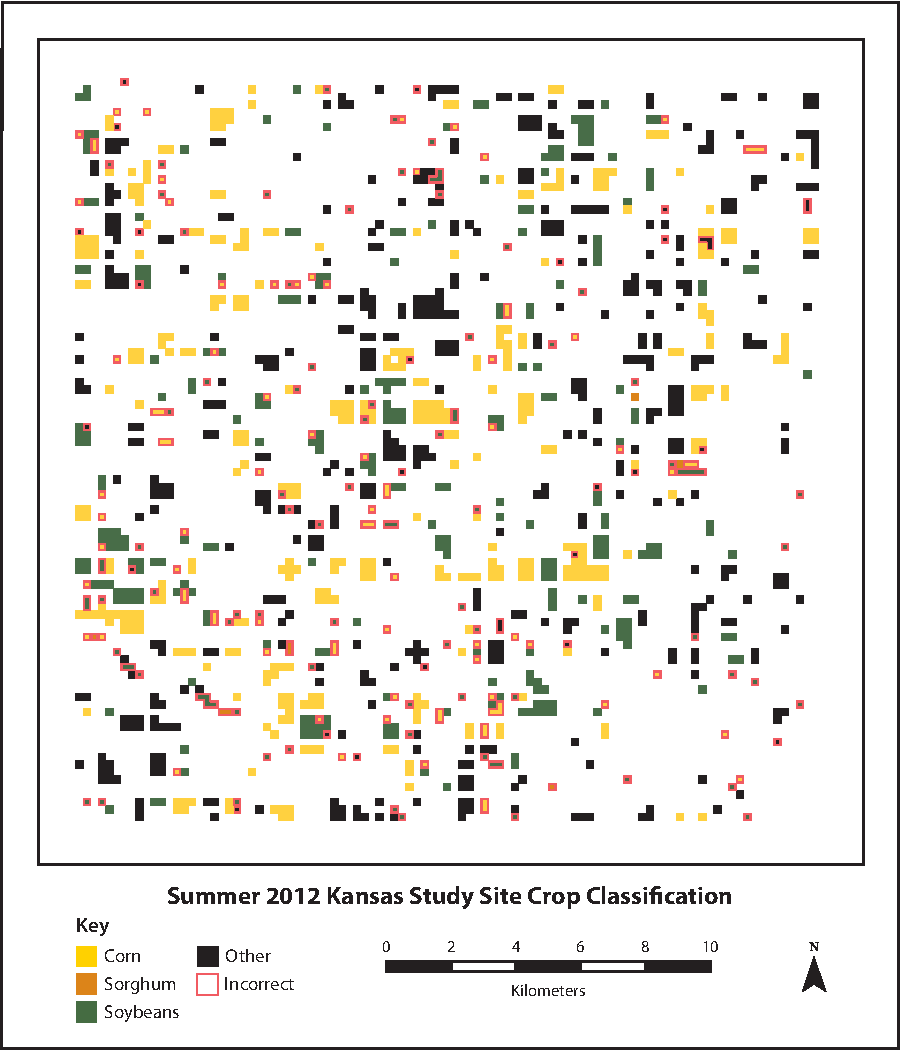
\includegraphics[width=0.55\textwidth]{Graphics/KSclass.pdf}
  %\caption[]{Kansas Summer 2012 Classification}
  %These are the results of classifying the summer 2012 Kansas TSI using corn, soy, and sorghum signatures. Incorrectly classified pixels are shown outlined in red. Omitted mixels were not symbolized, and appear white like the background.
\end{figure}
\end{frame}

\begin{frame}{Kansas Verification Classification}
\begin{table}
  \scriptsize
  \centering
  \caption{Summer 2012 Kansas Classification Accuracy}
  \begin{tabular}{rrrrrrrl}
    \toprule
    & & \multicolumn{4}{c}{\textbf{Reference Data}} & & \\
     &  & Corn & Soy & Sorghum & Other & Total & User Acc. \\
    \midrule
    \multirow{4}{*}{\rotatebox{90}{\textbf{Classified}}} & Corn & 369 & 65 & 5 & 17 & 456 & 80.92\% \\
     & Soy & 32 & 273 & 10 & 47 & 362 & 75.41\% \\
     & Sorghum & 0 & 0 & 2 & 6 & 8 & 25.00\% \\
     & Other & 13 & 16 & 1 & 503 & 533 & 94.37\% \\
    \addlinespace
     & Total & 414 & 354 & 18 & 573 & 1359 &  \\
    \addlinespace
    \multicolumn{2}{r}{Producer Acc.} & 89.13\% & 77.12\% & 11.11\% & 87.78\% &  &  \\
    \addlinespace
    \multicolumn{8}{r}{Overall Accuracy: 84.40\%} \\
    \multicolumn{8}{r}{Kappa: 0.76} \\
    \bottomrule
  \end{tabular}
\end{table}
\end{frame}

\begin{frame}{Kansas Verification Classification}
\begin{table}
  \centering
  \caption{\parbox{2in}{\centering~Kansas Classification RMSE Thresholds}}
  \begin{tabular}{lr}
    \toprule
    \Book{Signature} & \Book{Threshold Value} \\
    \midrule
    Corn\_1 & 1000 \\
    Corn\_2 & 750 \\
    \action<1-|alert@2>{Corn\_3} & \action<1-|alert@2>{500} \\
    Soy\_1 & 750 \\
    Soy\_2 & 1300 \\
    \action<1-|alert@2>{Soy\_3} & \action<1-|alert@2>{500} \\
    \action<1-|alert@2>{Sorghum} & \action<1-|alert@2>{450} \\
    \bottomrule
  \end{tabular}
\end{table}
\end{frame}


\subsection{Pellegrini Classification}
\begin{frame}{Pellegrini Classification}
\begin{table}
  \scriptsize
  \centering
  \caption{Summer 2014 Pellegrini Classification Accuracy}
  \begin{tabular}{rrrrrrrl}
    \toprule
     & & \multicolumn{4}{c}{\textbf{Reference Data}} & & \\
     &  & Corn & Soy & Sorghum & Other & Total & User Acc. \\
    \midrule
    \multirow{4}{*}{\rotatebox{90}{\textbf{Classified}}} & Corn & 24 & 13 & 0 & 8 & 45 & 53.33\% \\
     & Soy & 0 & 2 & 1 & 2 & 5 & 40.00\% \\
     & Sorghum & 0 & 0 & 0 & 0 & 0 & 0.00\% \\
     & Other & 12 & 9 & 1 & 306 & 328 & 93.29\% \\
    \addlinespace
     & Total & 36 & 24 & 2 & 316 & 378 &  \\
    \addlinespace
    \multicolumn{2}{r}{Producer Acc.} & 66.67\% & 8.33\% & 0.00\% & 96.84\% &  &  \\
    \addlinespace
    \multicolumn{8}{r}{Overall Accuracy: 87.83\%} \\
    \multicolumn{8}{r}{Kappa: 0.54} \\
    \bottomrule
  \end{tabular}
\end{table}
\end{frame}

\begin{frame}{Pellegrini Classification}
\begin{table}
  \centering
  \caption{Pellegrini Best Classification RMSE Thresholds}
  \begin{tabular}{lr}
    \toprule
    \Book{Signature} & \Book{Threshold Value} \\
    \midrule
    Corn\_1 & 550 \\
    Corn\_2 & 850 \\
    \action<1-|alert@2>{Corn\_3} & \action<1-|alert@2>{0} \\
    \action<1-|alert@2>{Soy\_1} & \action<1-|alert@2>{0} \\
    Soy\_2 & 600 \\
    Soy\_3 & 950 \\
    \action<1-|alert@2>{Sorghum\_1} & \action<1-|alert@2>{0} \\
    \bottomrule
  \end{tabular}
\end{table}
\end{frame}

\begin{frame}{Pellegrini Classification}
\begin{figure}
  \centering
  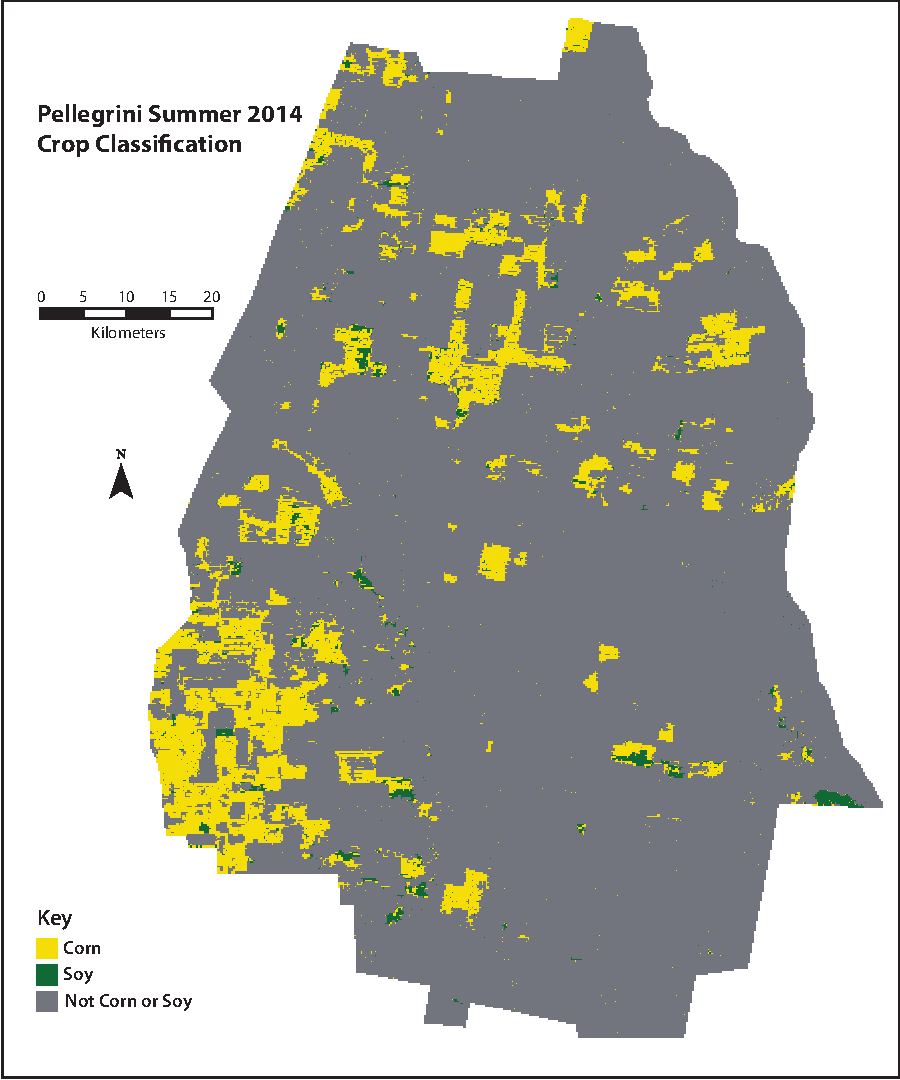
\includegraphics[width=0.53\textwidth]{Graphics/ARclassed.pdf}
  %\caption[Pellegrini Summer 2014 Classification]{Pellegrini Summer 2014 Classification}
  %Comparing this map to the ground truth in \cref{map:pellegrini:groundtruth} on \cpageref{map:pellegrini:groundtruth}, one can see how well the classification was able to separate soy and corn fields from the other classes. However, those fields are overwhelmingly classified as corn, suggesting major class confusion between the two. 
\end{figure}
\end{frame}


% CONCLUSION
\section{Conclusion}



%\begin{frame}{Systemvoraussetzungen}
%	Um erfolgreich Präsentationen mit diesem Theme erstellen zu können, sind folgende Voraussetzungen vom System zu erfüllen:
%	\begin{itemize}
%		\item Zum Setzen der Folien muss XeTeX verwendet werden.
%		\item Neben einigen Standardpaketen müssen die Pakete \texttt{beamer}, \texttt{pgf} und \texttt{xcolor} installiert sein.
%		\item Die Schriften \quoted{Flama-Light}, \quoted{Flama-Book} und \quoted{Flama-Medium} sollten installiert sein. Alternativ: \quoted{Arial}\\\url{http://www.felicianotypefoundry.com/}
%	\end{itemize}
%\end{frame}
%
%\section{Tutorial}
%\begin{frame}[containsverbatim]{Grundaufbau des Dokuments}
%Der Grundaufbau ist einfach:
%\begin{lstlisting}
%\documentclass[compress]{beamer}
%% Theme laden
%\usetheme{hsrm}
%% Allgemeine Präsentationseinstellungen 
%\title{Titel der Präsentation}
%\subtitle{Untertitel der Präsentation}
%\author{Ihr Name}
%\institute{Studienbereich\\Hochschule {\Medium RheinMain}}
%\begin{document}
%% Folien
%\end{document}
%\end{lstlisting}
%\end{frame}
%
%\begin{frame}{Themeoptionen}
%Um die Darstellung der Präsentation anzupassen können die folgenden Optionen gewählt werden.
%\begin{table}[]
%	\begin{tabularx}{\linewidth}{l>{\raggedright}X}
%		\toprule
%		\textbf{Option}			& \textbf{Auswirkung} \tabularnewline
%		\midrule
%		\texttt{noflama}		& Falls Sie die Schrift Flama nicht besitzen können Sie mit dieser Option auf die Schrift Arial umschalten. \tabularnewline
%		\texttt{noserifmath}		& Formeln werden ebenfalls serifenlos gesetzt. \tabularnewline
%		\texttt{nosectionpages} & Die Sektionseinleitungsseiten werden ausgeblendet.\tabularnewline
%		\bottomrule
%	\end{tabularx}
%	\label{tab:options}
%\end{table}
%\end{frame}
%
%\begin{frame}{Primärfarben}									
%Alle Farben des Corporate Designs sind im Template hinterlegt.
%
%
%\begin{multicols}{2}
%
%\setbeamercolor{hsrmRedDemo}{fg=hsrmRed,bg=white}
%\begin{beamercolorbox}[wd=\linewidth,ht=2ex,dp=0.7ex]{hsrmRedDemo}
%	\texttt{hsrmRed}
%\end{beamercolorbox}
%\setbeamercolor{hsrmRedDarkDemo}{fg=hsrmRedDark,bg=white}
%\begin{beamercolorbox}[wd=\linewidth,ht=2ex,dp=0.7ex]{hsrmRedDarkDemo}
%	\texttt{hsrmRedDark}
%\end{beamercolorbox}
%\setbeamercolor{hsrmWarmGreyDarkDemo}{fg=hsrmWarmGreyDark,bg=white}
%\begin{beamercolorbox}[wd=\linewidth,ht=2ex,dp=0.7ex]{hsrmWarmGreyDarkDemo}
%	\texttt{hsrmWarmGreyDark}
%\end{beamercolorbox}
%\setbeamercolor{hsrmWarmGreyLightDemo}{fg=hsrmWarmGreyLight,bg=white}
%\begin{beamercolorbox}[wd=\linewidth,ht=2ex,dp=0.7ex]{hsrmWarmGreyLightDemo}
%	\texttt{hsrmWarmGreyLight}
%\end{beamercolorbox}
%
%\setbeamercolor{hsrmRedDemoBg}{fg=white,bg=hsrmRed}
%\begin{beamercolorbox}[wd=\linewidth,ht=2ex,leftskip=.5ex,dp=0.7ex]{hsrmRedDemoBg}
%	\texttt{hsrmRed}
%\end{beamercolorbox}
%\setbeamercolor{hsrmRedDarkDemoBg}{fg=white,bg=hsrmRedDark}
%\begin{beamercolorbox}[wd=\linewidth,ht=2ex,leftskip=.5ex,dp=0.7ex]{hsrmRedDarkDemoBg}
%	\texttt{hsrmRedDark}
%\end{beamercolorbox}
%\setbeamercolor{hsrmWarmGreyDarkDemo}{fg=white,bg=hsrmWarmGreyDark}
%\begin{beamercolorbox}[wd=\linewidth,ht=2ex,leftskip=.5ex,dp=0.7ex]{hsrmWarmGreyDarkDemo}
%	\texttt{hsrmWarmGreyDark}
%\end{beamercolorbox}
%\setbeamercolor{hsrmWarmGreyLightDemo}{fg=white,bg=hsrmWarmGreyLight}
%\begin{beamercolorbox}[wd=\linewidth,ht=2ex,leftskip=.5ex,dp=0.7ex]{hsrmWarmGreyLightDemo}
%	\texttt{hsrmWarmGreyLight}
%\end{beamercolorbox}
%
%\end{multicols}
%
%\end{frame}
%
%\begin{frame}{Sekundärfarben}
%\begin{multicols}{2}
%
%\setbeamercolor{hsrmSec1Demo}{fg=hsrmSec1,bg=white}
%\begin{beamercolorbox}[wd=\linewidth,ht=2ex,dp=0.7ex]{hsrmSec1Demo}
%	\texttt{hsrmSec1}
%\end{beamercolorbox}
%\setbeamercolor{hsrmSec1DarkDemo}{fg=hsrmSec1Dark,bg=white}
%\begin{beamercolorbox}[wd=\linewidth,ht=2ex,dp=0.7ex]{hsrmSec1DarkDemo}
%	\texttt{hsrmSec1Dark}
%\end{beamercolorbox}
%\setbeamercolor{hsrmSec1CompDemo}{fg=hsrmSec1Comp,bg=white}
%\begin{beamercolorbox}[wd=\linewidth,ht=2ex,dp=0.7ex]{hsrmSec1CompDemo}
%	\texttt{hsrmSec1Comp}
%\end{beamercolorbox}
%\setbeamercolor{hsrmSec1CompDarkDemo}{fg=hsrmSec1CompDark,bg=white}
%\begin{beamercolorbox}[wd=\linewidth,ht=2ex,dp=0.7ex]{hsrmSec1CompDarkDemo}
%	\texttt{hsrmSec1CompDark}
%\end{beamercolorbox}
%
%\setbeamercolor{hsrmSec2Demo}{fg=hsrmSec2,bg=white}
%\begin{beamercolorbox}[wd=\linewidth,ht=2ex,dp=0.7ex]{hsrmSec2Demo}
%	\texttt{hsrmSec2}
%\end{beamercolorbox}
%\setbeamercolor{hsrmSec2DarkDemo}{fg=hsrmSec2Dark,bg=white}
%\begin{beamercolorbox}[wd=\linewidth,ht=2ex,dp=0.7ex]{hsrmSec2DarkDemo}
%	\texttt{hsrmSec2Dark}
%\end{beamercolorbox}
%\setbeamercolor{hsrmSec2CompDemo}{fg=hsrmSec2Comp,bg=white}
%\begin{beamercolorbox}[wd=\linewidth,ht=2ex,dp=0.7ex]{hsrmSec2CompDemo}
%	\texttt{hsrmSec2Comp}
%\end{beamercolorbox}
%\setbeamercolor{hsrmSec2CompDarkDemo}{fg=hsrmSec2CompDark,bg=white}
%\begin{beamercolorbox}[wd=\linewidth,ht=2ex,dp=0.7ex]{hsrmSec2CompDarkDemo}
%	\texttt{hsrmSec2CompDark}
%\end{beamercolorbox}
%
%\setbeamercolor{hsrmSec3Demo}{fg=hsrmSec3,bg=white}
%\begin{beamercolorbox}[wd=\linewidth,ht=2ex,dp=0.7ex]{hsrmSec3Demo}
%	\texttt{hsrmSec3}
%\end{beamercolorbox}
%\setbeamercolor{hsrmSec3DarkDemo}{fg=hsrmSec3Dark,bg=white}
%\begin{beamercolorbox}[wd=\linewidth,ht=2ex,dp=0.7ex]{hsrmSec3DarkDemo}
%	\texttt{hsrmSec3Dark}
%\end{beamercolorbox}
%\setbeamercolor{hsrmSec3CompDemo}{fg=hsrmSec3Comp,bg=white}
%\begin{beamercolorbox}[wd=\linewidth,ht=2ex,dp=0.7ex]{hsrmSec3CompDemo}
%	\texttt{hsrmSec3Comp}
%\end{beamercolorbox}
%\setbeamercolor{hsrmSec3CompDarkDemo}{fg=hsrmSec3CompDark,bg=white}
%\begin{beamercolorbox}[wd=\linewidth,ht=2ex,dp=0.7ex]{hsrmSec3CompDarkDemo}
%	\texttt{hsrmSec3CompDark}
%\end{beamercolorbox}
%
%\setbeamercolor{hsrmSec1DemoBg}{fg=white,bg=hsrmSec1}
%\begin{beamercolorbox}[wd=\linewidth,ht=2ex,leftskip=.5ex,dp=0.7ex]{hsrmSec1DemoBg}
%	\texttt{hsrmSec1}
%\end{beamercolorbox}
%\setbeamercolor{hsrmSec1DarkDemoBg}{fg=white,bg=hsrmSec1Dark}
%\begin{beamercolorbox}[wd=\linewidth,ht=2ex,leftskip=.5ex,dp=0.7ex]{hsrmSec1DarkDemoBg}
%	\texttt{hsrmSec1Dark}
%\end{beamercolorbox}
%\setbeamercolor{hsrmSec1CompDemoBg}{fg=white,bg=hsrmSec1Comp}
%\begin{beamercolorbox}[wd=\linewidth,ht=2ex,leftskip=.5ex,dp=0.7ex]{hsrmSec1CompDemoBg}
%	\texttt{hsrmSec1Comp}
%\end{beamercolorbox}
%\setbeamercolor{hsrmSec1CompDarkDemoBg}{fg=white,bg=hsrmSec1CompDark}
%\begin{beamercolorbox}[wd=\linewidth,ht=2ex,leftskip=.5ex,dp=0.7ex]{hsrmSec1CompDarkDemoBg}
%	\texttt{hsrmSec1CompDark}
%\end{beamercolorbox}
%
%\setbeamercolor{hsrmSec2DemoBg}{fg=white,bg=hsrmSec2}
%\begin{beamercolorbox}[wd=\linewidth,ht=2ex,leftskip=.5ex,dp=0.7ex]{hsrmSec2DemoBg}
%	\texttt{hsrmSec2}
%\end{beamercolorbox}
%\setbeamercolor{hsrmSec2DarkDemoBg}{fg=white,bg=hsrmSec2Dark}
%\begin{beamercolorbox}[wd=\linewidth,ht=2ex,leftskip=.5ex,dp=0.7ex]{hsrmSec2DarkDemoBg}
%	\texttt{hsrmSec2Dark}
%\end{beamercolorbox}
%\setbeamercolor{hsrmSec2CompDemoBg}{fg=white,bg=hsrmSec2Comp}
%\begin{beamercolorbox}[wd=\linewidth,ht=2ex,leftskip=.5ex,dp=0.7ex]{hsrmSec2CompDemoBg}
%	\texttt{hsrmSec2Comp}
%\end{beamercolorbox}
%\setbeamercolor{hsrmSec2CompDarkDemoBg}{fg=white,bg=hsrmSec2CompDark}
%\begin{beamercolorbox}[wd=\linewidth,ht=2ex,leftskip=.5ex,dp=0.7ex]{hsrmSec2CompDarkDemoBg}
%	\texttt{hsrmSec2CompDark}
%\end{beamercolorbox}
%
%\setbeamercolor{hsrmSec3Demo}{fg=white,bg=hsrmSec3}
%\begin{beamercolorbox}[wd=\linewidth,ht=2ex,leftskip=.5ex,dp=0.7ex]{hsrmSec3Demo}
%	\texttt{hsrmSec3}
%\end{beamercolorbox}
%\setbeamercolor{hsrmSec3DarkDemo}{fg=white,bg=hsrmSec3Dark}
%\begin{beamercolorbox}[wd=\linewidth,ht=2ex,leftskip=.5ex,dp=0.7ex]{hsrmSec3DarkDemo}
%	\texttt{hsrmSec3Dark}
%\end{beamercolorbox}
%\setbeamercolor{hsrmSec3CompDemo}{fg=white,bg=hsrmSec3Comp}
%\begin{beamercolorbox}[wd=\linewidth,ht=2ex,leftskip=.5ex,dp=0.7ex]{hsrmSec3CompDemo}
%	\texttt{hsrmSec3Comp}
%\end{beamercolorbox}
%\setbeamercolor{hsrmSec3CompDarkDemo}{fg=white,bg=hsrmSec3CompDark}
%\begin{beamercolorbox}[wd=\linewidth,ht=2ex,leftskip=.5ex,dp=0.7ex]{hsrmSec3CompDarkDemo}
%	\texttt{hsrmSec3CompDark}
%\end{beamercolorbox}
%
%\end{multicols}
%\end{frame}
%
%\begin{frame}[containsverbatim]{Folienstruktur}
%Strukturiert wird in Beamer wie in \LaTeX\ üblich mittels \lstinline!section!, \lstinline!subsection!, usw. Für Folien ist die \lstinline!frame! Umgebung definiert.
%
%Der Folientitel kann direkt an die \lstinline!frame! Umgebung übergeben werden oder mittels \lstinline!\frametitle{Folientitel}! innerhalb der Umgebung gesetzt werden.
%\begin{lstlisting}
%\section{Meine Sektion}
%\subsection{Meine Subsektion}
%\begin{frame}
%\frametitle{Folientitel}
%% Folieninhalt
%\end{frame}
%\end{lstlisting}
%\end{frame}
%
%\begin{frame}[containsverbatim]{Titelseite und Inhaltsverzeichnis}
%Die Titelseite erzeugt man mit 
%\begin{lstlisting}
%\maketitle
%\end{lstlisting}
%Und das Inhaltsverzeichnis mit
%\begin{lstlisting}
%\begin{frame}{Gliederung}
%	\tableofcontents[hideallsubsections]
%\end{frame}
%\end{lstlisting}
%Die Option \lstinline!hideallsubsections! bietet sich bei längeren Präsentationen an, um das Inhaltsverzeichnis kompakt zu halten.
%\end{frame}
%
%\subsection{Aufzählungen}
%\begin{frame}[containsverbatim]{Aufzählungen}
%Aufzählungen sind mit der \lstinline!enumerate! und der \lstinline!itemize! Umgebung möglich.
%\begin{enumerate}
%	\item Punkt 1
%	\item Punkt 2
%	\begin{itemize}
%		\item Punkt 1
%		\item Punkt 2
%	\end{itemize}
%	\item Punkt 3
%\end{enumerate}
%\end{frame}
%
%\subsection{Hervorhebungen}
%\begin{frame}[containsverbatim]{Hervorhebungen}
%In der Beamer Klasse ist die Funktion \lstinline!\alert! definiert, um einzelne Wörter hervorzuheben. Beispiel:
%\begin{itemize}
%	\item \alert{hervorgehobener Text}
%\end{itemize}
%Zusätzlich sind im HSRM Theme noch \lstinline!\quoted! und \lstinline!\doublequoted! definiert, um die Anführungszeichen des Corporate Designs der Hochschule einfach im Zugriff zu haben. Beispiele:
%\begin{itemize}
%	\item[] \quoted{Einfache Anführungszeichen}
%	\item[] \doublequoted{Doppelte Anführungszeichen}
%\end{itemize}
%\end{frame}
%
%\subsection{Blockstrukturen}
%\begin{frame}[containsverbatim]{Einfacher Block mit Aufzählung}
%Zur Strukturierung sind in Beamer Blockumgebungen definiert.
%\begin{block}{Block mit einer Aufzählung}
%	\begin{itemize}
%		\item Punkt 1
%		\item Punkt 2
%	\end{itemize}
%\end{block}
%\begin{lstlisting}
%\begin{block}{Block mit einer Aufzählung}
%	\begin{itemize}
%		\item Punkt 1
%		\item Punkt 2
%	\end{itemize}
%\end{block}
%\end{lstlisting}
%\end{frame}
%
%\begin{frame}[containsverbatim]{Alert Block}
%\begin{alertblock}{Alert Block}
%	Ein Alert Block wird mit der ersten Primärfarbe eingefärbt.
%\end{alertblock}
%\begin{lstlisting}
%\begin{alertblock}{Alert Block}
%Ein Alert Block wird mit der ersten Primärfarbe eingefärbt.
%\end{alertblock}
%\end{lstlisting}
%\end{frame}
%
%\begin{frame}[containsverbatim]{Example Block}
%\begin{exampleblock}{Example Block}
%	Ein Example Block wird mit der ersten Sekundärfarbe eingefärbt.
%\end{exampleblock}
%\begin{lstlisting}
%\begin{exampleblock}{Example Block}
%Ein Example Block wird mit der ersten Sekundärfarbe eingefärbt.
%\end{exampleblock}
%\end{lstlisting}
%\end{frame}
%
%\begin{frame}[containsverbatim]{Block mit anderer Farbe}
%\begingroup
%\setbeamercolor{block title}{bg=hsrmSec2Dark}
%\setbeamercolor{block body}{bg=hsrmSec2}
%\begin{block}{Block mit anderer Farbe}
%	In diesem Block wird eine weitere Sekundärfarbe verwendet.
%\end{block}
%\endgroup
%\begin{lstlisting}
%\begingroup
%\setbeamercolor{block title}{bg=hsrmSec2Dark}
%\setbeamercolor{block body}{bg=hsrmSec2}
%\begin{block}{Block mit anderer Farbe}
%	In diesem Block wird ...
%\end{block}
%\endgroup
%\end{lstlisting}
%\end{frame}
%
%\section{Beispielfolien}
%\begin{frame}{Weitere Beispiele}
%Nachfolgend sind weitere Beispielfolien ohne zusätzliche Erläuterung angehängt.
%
%Schauen Sie einfach in den Quelltext, um zu sehen wie die Folien erstellt wurden.
%\end{frame}
%\subsection{Abbildungen}
%\begin{frame}{Foto mit Copyright}
%	\begin{figure}
%		\centering
%		\includegraphicscopyright[width=\linewidth]{photo.jpg}{Copyright by \href{http://netzlemming.deviantart.com/}{Netzlemming}, \href{http://creativecommons.org/licenses/by-nc/3.0/}{CC BY-NC 3.0 License}}
%	\end{figure}
%\end{frame}
%\begin{frame}{Plot mit Beschriftung}
%	\begin{figure}
%		\centering
%		\input{plot.tex}
%		\caption{LFE channel frequency spectrum}
%	\end{figure}
%\end{frame}
%
%\subsection{Tabellen}
%\begin{frame}{Tabelle}
%\begin{table}[]
%	\caption{Selection of window function and their properties}
%	\begin{tabular}[]{lrrr}
%		\toprule
%		\textbf{Window}			& \multicolumn{1}{c}{\textbf{First side lobe}}	
%		                    & \multicolumn{1}{c}{\textbf{3\,dB bandwidth}}
%		                    & \multicolumn{1}{c}{\textbf{Roll-off}} \\
%		\midrule
%		Rectangular				& 13.2\,dB	& 0.886\,Hz/bin	& 6\,dB/oct		\\[0.25em]
%		Triangular				& 26.4\,dB	& 1.276\,Hz/bin	& 12\,dB/oct	\\[0.25em]
%		Hann					& 31.0\,dB	& 1.442\,Hz/bin	& 18\,dB/oct	\\[0.25em]
%		Hamming					& 41.0\,dB	& 1.300\,Hz/bin	& 6\,dB/oct		\\
%		\bottomrule
%	\end{tabular}
%	\label{tab:WindowFunctions}
%\end{table}
%\end{frame}
%
%\subsection{Formeln}
%\begin{frame}{Formeln}
%\begin{block}{Fourierintegral}
%\begin{equation*}
%F(\textrm{j}\omega) = \int\limits_{-\infty}^{\infty} f(t)\cdot\textrm{e}^{-\textrm{j}\omega t} dt
%\end{equation*}
%\end{block}
%\begin{block}{Fakultät}
%\begin{equation*}
%	n! = 1\cdot 2 \cdot 3 \cdot\ldots\cdot n = \prod_{k=1}^n k
%\end{equation*}
%\end{block}
%\end{frame}
%
%\begin{frame}{Mindmap mit TikZ}
%\centering
%\begin{tikzpicture}[scale=0.88]
%	%\tikzset{every child/.append style={level distance=250}}
%	\path[mindmap,concept color=hsrmWarmGreyLight,text=hsrmWarmGreyDark]
%	node[concept] {\TeX}
%	[clockwise from=-30]
%	child[concept color=hsrmSec2Dark,text=white] { node[concept] {\textcolor{white}{\XeTeX}} }
%	child[concept color=hsrmSec1CompDark,text=white] { node[concept] {\ConTeXt} }
%	child[concept color=hsrmSec1Dark,text=white] { node[concept] {\LaTeX} };
%\end{tikzpicture}
%\end{frame}
%
%\subsection{Fußnoten}
%\begin{frame}{Fußnoten}
%	Lorem ipsum dolor sit amet, consetetur sadipscing elitr, sed diam nonumy eirmod tempor invidunt ut labore et dolore magna aliquyam erat, sed diam voluptua. At vero eos et accusam et justo duo dolores et ea rebum. Stet clita kasd gubergren, no sea takimata sanctus est Lorem ipsum dolor sit amet. Lorem \footnote[frame,1]{Lorem ipsum dolor sit amet} ipsum dolor sit amet, consetetur sadipscing elitr, sed diam nonumy eirmod tempor invidunt ut labore et dolore magna aliquyam erat, sed diam voluptua. At vero eos et accusam et justo duo dolores et ea rebum. Stet clita kasd gubergren, no sea takimata sanctus est Lorem ipsum dolor sit amet.
%\end{frame}
%
%\subsection{Notizen}
%\begin{frame}{Folie mit dazugehöriger Notizfolie}
%    Für das Publikum ist diese Folie.
%
%	Für ihre Präsentation bieten sich folgende Programme an:
%	\begin{itemize}
%		\item Splitshow (Mac OS X)\\\url{https://code.google.com/p/splitshow/}
%		\item pdf-presenter (Windows)\\\url{https://code.google.com/p/pdf-presenter/}
%	\end{itemize}
%\end{frame}
%
%\note{
%    Für Ihre Notizen zum Vortrag vewenden Sie diese Folie.
%    
%	Für ihre Präsentation bieten sich folgende Programme an:
%	\begin{itemize}
%		\item Splitshow (Mac OS X)\\\url{https://code.google.com/p/splitshow/}
%		\item pdf-presenter (Windows)\\\url{https://code.google.com/p/pdf-presenter/}
%	\end{itemize} 
%}
%
%\subsection{Spalten}
%\begin{frame}{Zwei Spalten}
%	\begin{multicols}{2}
%		Lorem ipsum dolor sit amet, consetetur sadipscing elitr, sed diam nonumy eirmod tempor invidunt ut labore et dolore magna aliquyam erat, sed diam voluptua. At vero eos et accusam et justo duo dolores et ea rebum. Stet clita kasd gubergren, no sea takimata sanctus est Lorem ipsum dolor sit amet.
%		\begin{itemize}
%        	\item ein Eintrag
%        	\item noch ein Eintrag
%		\end{itemize}
%	\end{multicols}
%\end{frame}
%
%\begin{frame}{Spaltenumbruch}
%	\begin{multicols}{2}
%		Lorem ipsum dolor sit amet, consetetur sadipscing elitr, sed diam nonumy eirmod tempor invidunt ut labore et dolore magna aliquyam erat, sed diam voluptua. At vero eos et accusam et justo duo dolores et ea rebum. Stet clita kasd gubergren, no sea takimata sanctus est Lorem ipsum dolor sit amet.
%		\columnbreak
%		\begin{itemize}
%        	\item ein Eintrag
%        	\item noch ein Eintrag
%		\end{itemize}
%	\end{multicols}
%\end{frame}
%
%\begin{frame}{Literaturverzeichnis}
%	\begin{thebibliography}{10}
%    
%	\beamertemplatebookbibitems
%	\bibitem{Oppenheim2009}
%	Alan~V.~Oppenheim
%	\newblock \doublequoted{Discrete-Time Signal Processing}
%	\newblock Prentice Hall Press, 2009
%
%	\beamertemplatearticlebibitems
%	\bibitem{EBU2011}
%	European~Broadcasting~Union
%	\newblock \doublequoted{Specification of the Broadcast Wave Format (BWF)}
%	\newblock 2011
%  \end{thebibliography}
%\end{frame}
%
%\section{Ausblick}
%\begin{frame}{Bekannte Fehler}
%	\begin{itemize}
%		\item Theme ist momentan noch in einer einzelnen sty-Datei. Diese sollte unterteilt werden in einzelne Dateien für Schrift, Farbe usw.
%	\end{itemize}
%\end{frame}
%
%\begin{frame}{Fragen, Anmerkungen, Kontakt}
%	Das HSRM Theme steht unter der \quoted{GNU Public License}. Es darf also weitergegeben und modifiziert werden, sofern die Lizenzart beibehalten wird.
%	
%	Für Fragen und Anmerkungen stehe ich gerne zur Verfügung.
%	\begin{itemize}
%		\item \url{Benjamin.Weiss@student.hs-rm.de}
%	\end{itemize}
%\end{frame}

\end{document}






